\documentclass[11pt,twoside]{report}
\usepackage[a4paper,width=160mm,top=20mm,bottom=20mm,bindingoffset=6mm]{geometry}

\usepackage{amsthm}
\usepackage{amsfonts}
\usepackage{amsmath,amssymb}
\usepackage{graphicx}
\usepackage{wrapfig}
\usepackage[T1]{fontenc} 
\usepackage[utf8]{inputenc}
\usepackage{graphicx}
\usepackage{wrapfig}
\usepackage{mathtools} 
\usepackage{lipsum}
\usepackage{color}
\usepackage[english]{babel}
\usepackage{appendix}
\usepackage{float}
\usepackage{enumitem}
\usepackage{setspace}
\usepackage{subcaption}
\usepackage{amssymb}
\usepackage{fancyhdr}
\usepackage{titlesec}
\usepackage{mathrsfs}
\usepackage[ruled,vlined]{algorithm2e}

\titleformat{\chapter}[display]
{\normalfont\huge\bfseries}{\chaptertitlename~\thechapter}{20pt}{\Huge}
\titlespacing*{\chapter}{0pt}{30pt}{15pt}
\titlespacing*{name=\chapter,numberless}{0pt}{-30pt}{10pt}

\newenvironment{system}
{\left\lbrace\begin{array}{*{4}{c@{}>{{}}c<{{}}@{}}c}}
	{\end{array}\right.}
\setlength{\parindent}{0pt}

\makeatletter
\@addtoreset{section}{part}
\makeatother
\renewcommand{\partname}{}
\linespread{0.75}
\newcommand\independent{\protect\mathpalette{\protect\independenT}{\perp}}
\def\independenT#1#2{\mathrel{\rlap{$#1#2$}\mkern2mu{#1#2}}}
\let\oldemptyset\emptyset
\let\emptyset\varnothing
\singlespacing
\newtheorem{definition}{Definition}
\newtheorem{lemma}{Lemma}
\newtheorem{prop}{Proposition}
\newtheorem{model}{Model}

\begin{document}
	
\pagenumbering{gobble}
\vspace*{-1.5cm}{
	\begin{center}
		\large
		POLITECNICO DI MILANO\\
		\normalsize
		Master Degree in Mathematical Engineering\\
		Industrial and Information Engineering\\
		Department of Mathematics\\
		\begin{figure}[htbp]
			\begin{center}
				
\includegraphics[width=3.5cm]{./pictures/logo.jpg}
			\end{center}
		\end{figure}
		\vspace*{0.3cm} \LARGE
		
		
		
		\textbf{A Bayesian model for data flow: BikeMi}\\
		
		
		\vspace*{.75truecm}\large
		\vspace*{.5truecm} \large
		052499 - Bayesian Statistics Project Report
	\end{center}
	\vspace*{3.0cm} \large
	\begin{flushleft}
		
		
		Professor: Alessandra Guglielmi \\
		Professor: Riccardo Corradin \\
		Project Tutor: Mario Beraha
		
	\end{flushleft}
	\vspace*{3.0cm}
	\begin{flushright}
		
		
		Group members:\\
		Andrea De Gobbis \\
		Lorenzo Ghilotti \\
		Giorgio Meretti
		
		
	\end{flushright}
	\vspace*{2.0cm}
	\begin{center}
		
		
		
		Academic Year 2019-2020
	\end{center} \clearpage
}
\shipout\null

\pagenumbering{arabic} 
\pagestyle{fancy}
\fancyhf{}
\fancyhead{}
\fancyhead[RO,LE]{BikeMi -- add}
\fancyfoot{}
\fancyfoot[C,C]{\thepage}
\renewcommand{\headrulewidth}{0.4pt}

\tableofcontents{}

\chapter*{Introduction}
This project is the natural continuation of the work due to G. Bissoli, C. Principi, G. M. Rinaldi (BG19 in the bibliography), last year. But, whilst their goal was that of predicting the amount of traffic in a network independently of the particular day in which data have been registered, our main purpose will be developing a time series approach to the problem. We will obviously take advantage of some tools, like DBSCAN clusterization, already employed by our colleagues, but every time with a critical aproach, aiming to improve and possibly generalize the baseline already provided to us.\\
\\
In our project we will mainly focus on two targets: developing a global model able to predict the overall amount of traffic in the BikeMi network of Milan, being suitable for daily forecasts, and attempting to produce a network model to mimic the same ideas on the specific graph-based context. In light of these purposes, we will use fully Bayesian tools like loglinear models, Bayesian Structural Time Series (BSTS), spatial approaches and also some heuristics, like the penalized DBSCAN, to fasten computions. We don't have the ambition to produce outstanding results, given the relatively small amount of data at our disposal, but we hope - at least - to provide an introductory insight to the problem, possibly suggesting some methodological patterns and clever ideas to evolve models in this framework.

\chapter{Data preprocessing}
As already pointed out during the introduction, the data preprocessing performed in the original paper - that from now on will be addressed as Model Zero (M0) - was conceived like an elementary preliminary tool capable of creating a shrunk, tractable number of macro-nodes, vital precondition for the feasibility of an on-network Bayesian approach. However, the clusterig operation, carried out with the popular density-based frequentist algorithm DBSCAN, highlighted some critical issues that will be discussed in the first section of this chapter. As an introductory challenge for our project, we tried to improve the design of this early phase, developing a more contextualized - but still frequentist - version of the DBSCAN, in order to better capture the core-periphery structure of big round cities.

\section{Criticalities of a purely Euclidean DBSCAN}
Unquestionably, the primary goal of a location-based clustering is that of grouping  together nodes according to some spatial criterion. First of all, a definition of similariy must be established: clarifying what does it mean for two nodes to be in the same area. Then, the gathering has to be performed, condensing neighbouring locations in a unique baricenter, whose strength can be seen as the element-by-element sum of the connectivities of its members. The pure DBSCAN identifies the proximity of two nodes using their Euclidean distance and merges multiple locations according to this criterion.\\
\\
In principle, such a method may appear perfectly valid, but unfortunately it seems to overlook a crucial property of a spatial networks: the topology. When dealing with big cities, like Milan, there are some centers of interest which can't be totally neclected, since they tend to aggregate around them a massive traffic and, as a consequence, a bigger number of stations. However, a large-scale combination of these flows in a unique point appears plainly unwise, as an extreme counterexample just think about the damage produced by merging all the stations in a handful of macro-nodes. More in general, indiscriminate gruping increases considerably the risk of losing both interpretability of the streams and predictive potential. In light of this, we looked at the issue of employing something different from a common notion of distance, to better classify the closeness of two points in a net.\\
\\
But, as for the moment, let us just try to point out the main imperfections encountered in the analysis of M0, which in the end brought us to seek a way of improving it. Figure \ref{fig:old_model_gephi} shows the old aggregation with a Gephi representation. Just for the sake of readability, we describe here the criterion with which the graph has been plotted, taking into account that the same kind of style will be repeated through all the representations of this report. Nodes are marked by points in the graph: intuitively a big size, just like a hot color entails the presence of an hub - a node with many connections - viceversa small sizes or cold colors denote low strength nodes. To be precise the color is proportional to the degree of the nodes, i.e. the number of objects with which is direcly linked, while the radius is commensurate with the strength of the node, where each connection is weighted by the number of bikes running on it. Finally, the numbers over the nodes coincide with their id in the datatset if and only if they are positioned above an actually existing station. Conversely if the label exceeds 1000 we can treat the corresponding dot as the baricenter (according to the Euclidean distance) of some cluster achieved through the DBSCAN. Since the graph is directed, connections exist in both ways and are denoted by straight arrows. Again, the color is proportional to the strength of the corresponding flow (to be precise is linked to the in-degree of the flows entering inside some target node).

\begin{figure}[H]
	\begin{center}
		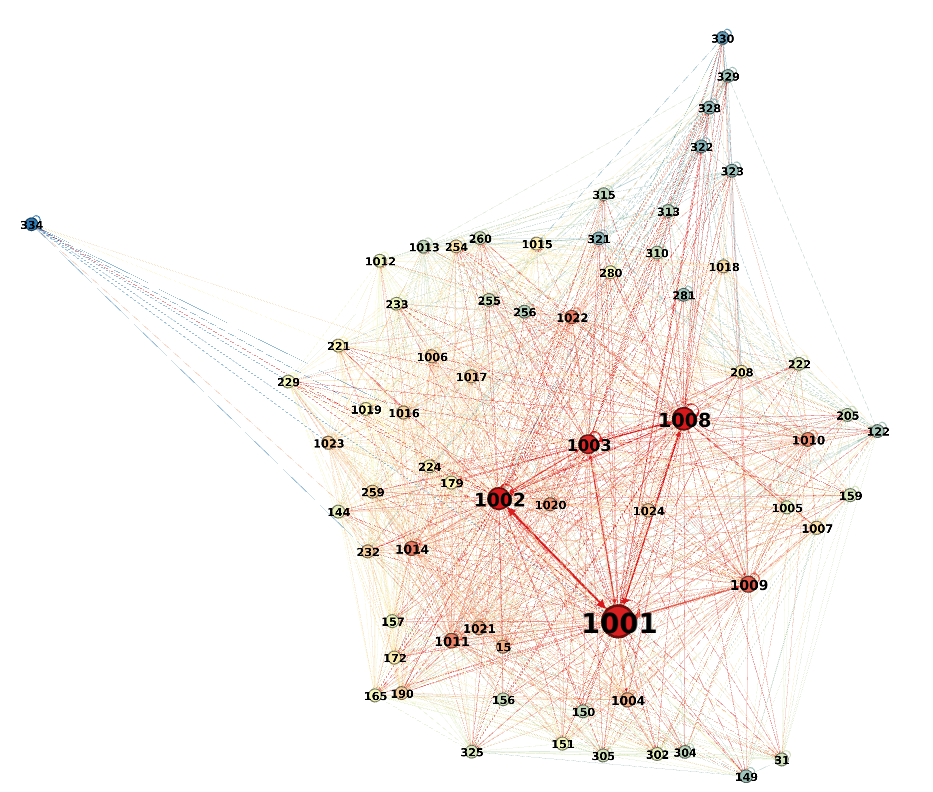
\includegraphics[width=15cm]{./pictures/old_model_gephi.png}
	\end{center}
	\caption{M0 nodal aggregation}
	\label{fig:old_model_gephi}
\end{figure}

We can immediatey notice something not perfectly balanced in this representation, especially if we compare it with the original graph before the preprocessing - where labels have been omitted for the sake of readability - in figure \ref{fig:original_graph_gephi}. The original structure presented a lot of average size highly connected stations in the center of the city, together with a small fraction of hubs (corresponding to the principal stations of Milan). On the other hand this topology is partially compressed and twisted in M0, where the city center and the main stations have been clustered with almost all their districts, creating a sort of autonomously behaving and self-centered quadrilateral given by nodes (1001-1002-1003-1008), whereas the preriphery is almost left untouched and filled with singletons (i.e. non clusterized nodes) characterized by poor connections and feeble strength. Practically speakingm M0 appears to be overaggregating the central area, lacking in capability to link stations in the more external districts. Obviously this is a side effect of how the DBSCAN (or in general a clustering algorithm) works if fed by a notion of similarity that is a distance, namely a mathematical relationship that - forced to satisfy the triangular inequality - is not able to capture a structure where neighbourhoods are somehow proportional to the distance from some key locations.\\
\\
To support our thesis concerning the partial inadequacy of M0, besides the graphic intuition, we have collected some quantities ponting out the problem, for instance:

\begin{figure}[H]
	\begin{center}
		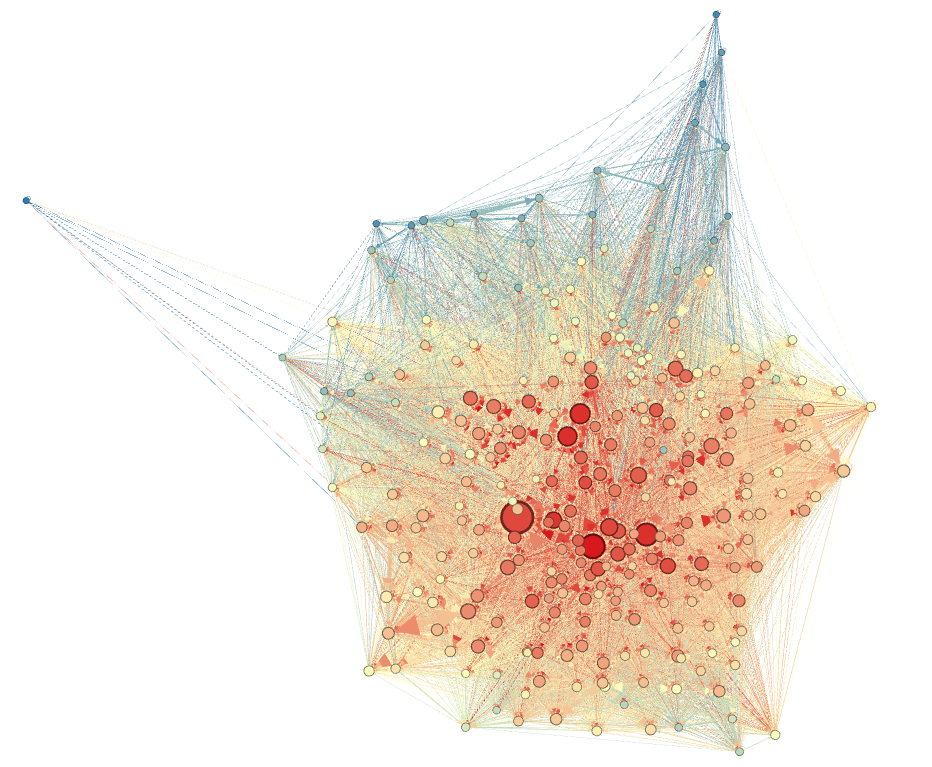
\includegraphics[width=15cm]{./pictures/original_graph_gephi.png}
	\end{center}
	\caption{Original network}
	\label{fig:original_graph_gephi}
\end{figure}

\begin{itemize}
	\item The loop percentage: dealing with networks, one may encounter many situations that require considering the presece of flow from a point to itself. This peculiar connection is called loop of a node. Notice that, in the BikeMi context, we can easily interpret this situation as the presence of people borrowing a bike for a small trip and later returning it to the same station. Moreover, loops are also an interesting analytic tool in this framework, since their comulative weighted percentage with respect to the total amount of links in the network can give advice about how many people on average tend to make "irrelevant" trips. Obviously, the insignificance has to be read from a managerial viewpoint, in the sense that after one loop the bikes in a station are just as many as before the - hopefully brief - period, in absence of other modifications. In the original dataset these rings amount to just around the 2\% of the links (to be accurate, $ P=1.78\% $).
	In the following picture \ref{fig:loop_distribution} it's possible to see the different loop percentages in each of the 258 nodes of the map, five outliers are removed: 229, 249, 329, 330, 334, actually some of the most peripheric stations. Notice also that the numerousness (out-strength $ S^{out}_i $) of these nodes, respectively 263, 339, 144, 71, 11 are far beyond the average as pointed out by their distribution \ref{fig:n_out_links}, hence it's safe to consider them quite irrelevant, since $ P = \sum_{i=1}^{263}S^{out}_iP_i $ as a weighted mean. Assuming the percentage of loops $ P_i $ r.v.s coming i.i.d. from the same population, we can see that $ P $ does not differ too much from the median of the common distribution for the $ P_i $, $ 1.75\% $, with 90\% of the empirical c.d.f. inside the interval $[0.63\%, 3.64\%]$, confirming the node-by-node roubustness of the average estimate represented by $ P $.\\
	\\
	Let us now consider what happens whenever merging together nodes in clusters: a possibly interesting collateral effect is making the average loop percentage non-decrease. Taking into account that an ideal merging of the nodes, although gathering spatially indistinguishable stations, shall never be allowed to modify the underlying topology of the network, a really effective clustering should have the tendency to aggregate nodes that are really close by, but without making the aforementioned $ P $ quantity explode. Let's see in detail how $ P $ reacts to clustering. Obviously, if two nodes $ N_1 $ and $ N_2 $ are coupled in a single cluster $ C = \{N_1,N_2\}$ the total number of loops  becomes $ L(C) = L(N_1) + L(N_2) + F(N_1\rightarrow N_2) + F(N_2\rightarrow N_1)$, where $ F(A\rightarrow B) $ denotes the flow from station $ A $ to $ B $. However, if two nodes are supposed to be part of the same macro-cluster, it might seem logical, also in tems of distribution,  to consider $F(N_1\rightarrow N_2)$ and $F(N_2\rightarrow N_1)$ exchangeable and close in value to the corresponding nodal loops (or even a bit smaller, since it would appear strange to see a person taking a bike to cover a distance in almost the same time that he would have spent by foot without check-in/out procedures and the risk of not being able to park in the target station). Hence, if the average size of a cluster in our grouping is $ G_* $ ($ G $ by default is 1), we expect a good clustering to satisfy a sublinear growth in $ G_* $, $ P_*\leq PG_*$. In M0, $ P_0=23.76\% $ and $ G_0= 3.93 $, the inequality is far from being met. This signal should be read as a warning: there is strong evedence to claim that M0 destroys the topological nature of the original structure, gathering together nodes very far one another, which should not be merged together.
	
	\begin{figure}[H]
		\begin{subfigure}[H]{0.5\linewidth}
			\centering
			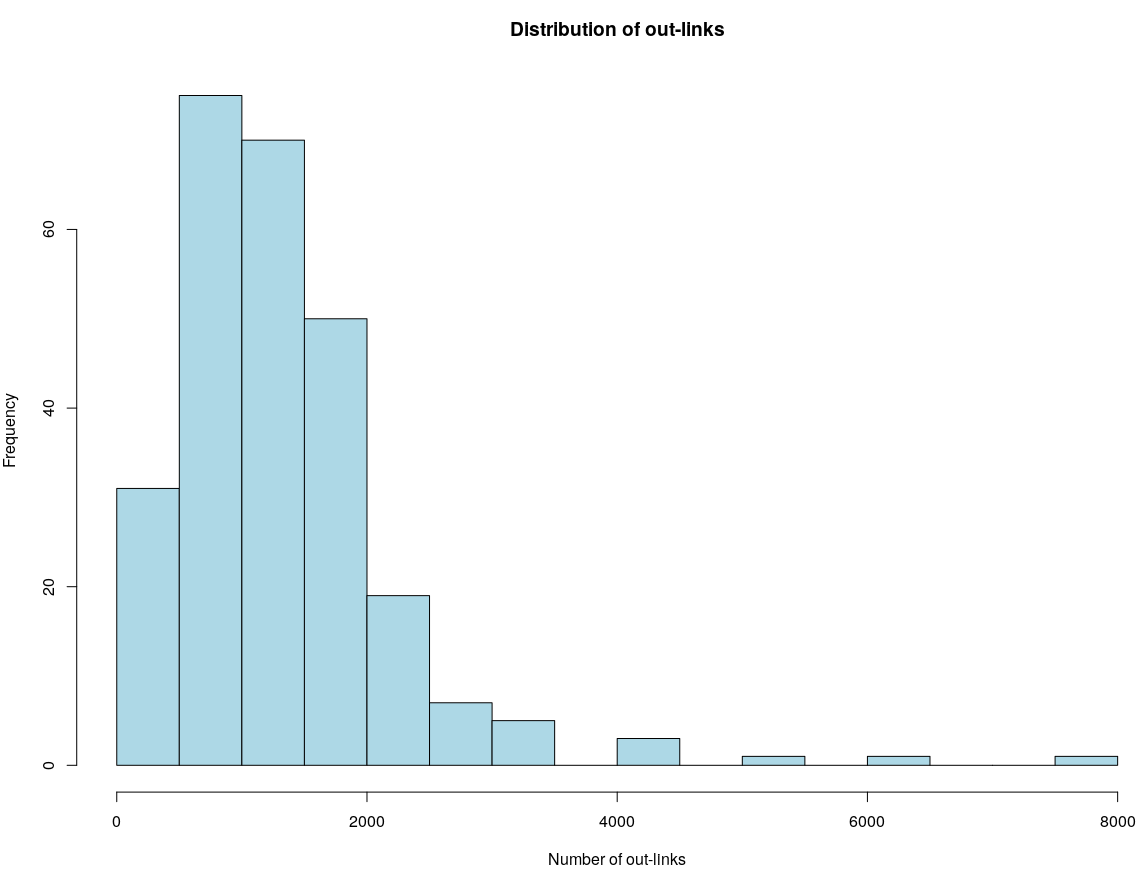
\includegraphics[width=70 mm]{pictures/number_out_links.png}
			\caption{Distribution of links}
			\label{fig:n_out_links}
		\end{subfigure}
		\hfill
		\begin{subfigure}[H]{0.5\linewidth}
			\centering
			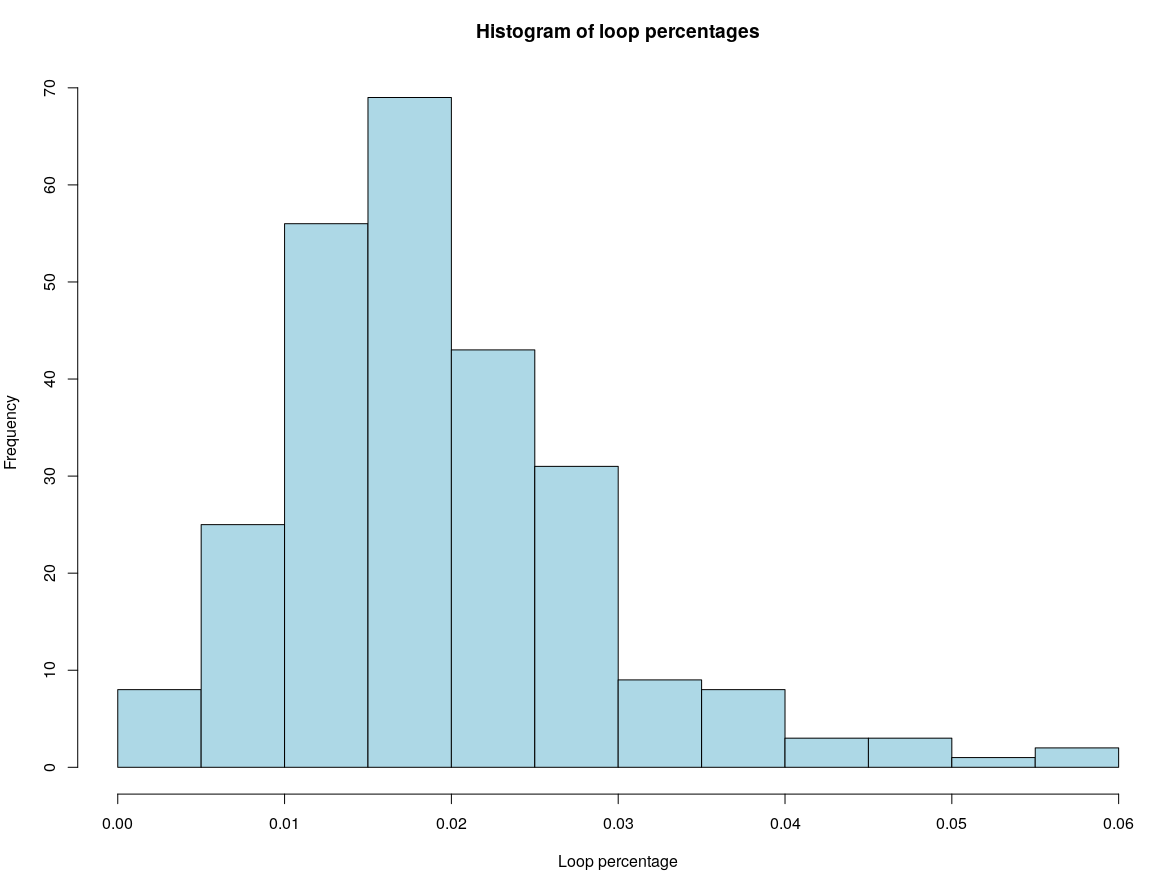
\includegraphics[width=70 mm]{pictures/loop_percentages_distribution.png}
			\caption{Histogram of loop percentages \\without outliers}
			\label{fig:loop_distribution}
		\end{subfigure}%
		\caption{Properties in the orginal dataset}
	\end{figure}
	
	\item The cluster dimensions: after M0 grouping, is of extreme importance to compare the size among distinct clusters. Indeed, a proper merging is expected to somehow create balanced groups, since sporadic high numerousness can be symptomatic of overaggregation. Unfortunatley, even though the number of singletons is quite low for the model (only 43, which is an excellent result) clusters 1001, 1002, 1003 and 1008 - respectively the whole city center, Cadorna, Garibaldi and Central railway stations - are pretty oversized compressing together 65, 25, 16, 41 nodes. Moreover, even though the distribution of loop percentages does not change dramaticaly, the variations reflect an improper behaviour. Under M0, the nodes with $ P^{0}_i $ exceeding the threshold, fixed at $ P^{opt}_i=12\% $ - almost $ G_0P $ - are still the peripheric unclusterized 330 and 334, but also clusters 1001, 1002, 1003, 1004, 1008 and 1009, whose cluster out-strength $ S^{0}_i $ are respectively 104144, 48979, 31113, 52672, 17549: i.e. are impossible to be neglected (actually they are the most relevant clusters of the dataset). Note also that groups concernig the city center, Cadorna and Centrale are far from being light outliers, with loop percentages respectively of 40.19\%, 23.68\% and 34.84\%.
\end{itemize}

Summing up: all our elementary analyses agree in spotting a certain tendency of M0 to overaggregate clusters around the citycenter, merging together too many nodes which often should be considered separately, but still leaving untouched many singletons in periphery.
From this starting point, we decided to look for a strategy able to unclusterize enourmous groups still preserving and possibly enhancing strong connectivity in the other merged regions.

\section{Penalized DBSCAN}
In this section we are going to present an upgraded version of the classic DBSCAN structure that we decided to employ in order to clusterize the nodes, both covering the main modifications, in particular the introduction of a penalised notion of distance, and discussing its pros and cons.

\subsection{The algorithm}
The basic idea employed in our work was that of feeding the DBSCAN algorithm with a similarity matrix produced, not by the standard Euclidean distance (denoted by $ ||x-y|| $, $ \forall x, y \in \mathbb{R}^2 $), but with a penalized vesion of it: $ smd(x,y) = \frac{p(y)+p(x)}{2}||x-y|| $, through a suitable non-negative function $ p(*) $. By costruction, $ smd(*,*) $ can be classified as a semi-distance: it is non-negative, symmetric and satisfies the annulment property. In general it won't meet the triangular inequality, unless under very implausible and out-of-context assumptions.\\
\\
The flexibility of the model is given by the freeedom of choice in the penalization, that we constructed in order to be adapted to a circular-shaped metropolis, like the city of Milan. The goal was that of forcing the DBSCAN algorithm to be more thrifty in the citycenter, to avoid overaggregation around the main monuments and business locations, whilst stimulating, on the other hand, a stronger clustering in periphery. Thus, a straightforward idea, at least under radial symmetry,  was that of a penalization function actually depending from the Euclidean distance between a certain node and the city center (identified by the exact geographical coordinates of the cathedral, $ x_0 $): i.e. $\exists g:[0,+\infty)\rightarrow[0,+\infty)$, non-increasing s.t. $p(x) = g(||x-x_0||),\ \forall x \in \mathbb{R}^2$.\\
\\
Under these assumptions, the problem lied in the identification of a suitable choice for $ g(*) $. We opted for a parametric family of functions, able to cover a wide-enough variety of shapes:
\begin{equation}
 g(u) = \max\{\beta, e^{(\frac{u}{\alpha})^2\log{(1-\gamma)}}+\gamma\}\ \ \forall u \in [0,+\infty)
\end{equation}
where $ \alpha>0,\ \beta\in[0,1],\ \gamma \in (0,1) $. It's easy to see that if $ \beta=0 $, $ g $ is a gaussian kernel, whose asymptotic value is given by $ \gamma $ and $ g(0)=1+\gamma $. $ \alpha $ is a shape parameter and identiefies the radius of the points with no penalization in the distance since $ g(\alpha)=1 $. $ \beta $ is the minimum scale factor employed in the problem, irrelevant if $ \beta<\gamma $. Finally, notice that all functions in the family are smooth - but, at most, a non differentiability point - non-negative and non-increasing.\\
\\
In order to make some automatic parameter selection without losing both the constraints and the magnitude $ \mathcal{O}(1) $ defined before, we decided first to normalize $ smd(x_i,x_j),\ \forall i,j \in {id}^2$ with the median of the distances between all the nodes and $ x_0 $, $ m=qt(||X -x_0||,0.5) $, defining $ smd'(x_i,x_j)=\frac{smd(x_i,x_j)}{m} $. Then, given this notion of similarity, it was possible to fix the penalization parameters on uniform grids of step $ \sim \frac{1}{20} $ of the correponding scale factor - e.g. if $ \gamma $ has scale $ 1=10^0 $, step $ =0.05 $ - later refined with some bisection. Since we were trying to establish the values for which the spatial aggregation best captured the net topology, to automatize the procedure, we decided to restrict the feasible models to a smaller subset of parametric combinations satisfying some minimal requirements $ \mathcal{C} $: weighted loop percentage $ P<15\% $, number of clusters $nc >40 $, percentage of singletons $ I<33\% $. Finally, we defined an empirical goodness-of-fit function $ GOF(m)=P(m)+3I(m) $ for each model $ m $, adapted to the expected optimal sizes of clusters, whose minimization selected the best parametric set as $ \hat{m}=\arg\min GOF(m) $.

\subsection{Results}
The model selected through the penalized DBSCAN has $ \alpha=0.8, \gamma=0.5 $. Since small values of $ \beta $ appear reasonable, we decided to force $ \beta=0 $ in order to simplify the computation of the penalization without a strong loss in terms of clustering power. To be precise we should add another detail: the standard DBSCAN  employed in our method needs two parameters in input: the minimum size of the accepted clusters - for us by default was 2 - and the radius $ \varepsilon $ of all the balls employed in the internal routines of the algorithm. For this second issue, given the normalization, we decided to use an $ \varepsilon \in[0.90, 1.15] $. However, there is no strong detectable discrepency in the highest values of this range, in particular we selected the upper bound 1.15.\\
\\
\begin{algorithm}[H]
	\SetAlgoLined
	Fix a center $ x_0 $;\\
	Fix $ \varepsilon=1.15 $;\\
	Compute $ m=t(||X -x_0||,0.5) $;\\
	\For{$ \alpha \in $ 0.1\ :\ 0.05\ :\ 0.9}
	{
		\For{$ \beta \in $ 0\ :\ 0.05\ :\ 1}
		{
			\For{$ \gamma \in $ 0.1\ :\ 0.05\ :\ 0.9}
			{
				 Compute penalization $ p(x) = \max\{\beta, e^{(\frac{||x-x0||}{\alpha})^2\log{(1-\gamma)}}+\gamma\} $ for each node $ x $;\\
				 Define matrix $ smd'(x,y) = \frac{p(y)+p(x)}{2}\frac{||x-y||}{m} $ for each node couple $ (x,y) $;\\
				 Compute DBSCAN($ sdm' $), 2, $\varepsilon$);\\
				\eIf{$ C $ is $ \mathtt{true} $}{
					Save iteration;\\
					Compute $ GOF(\alpha,\beta,\gamma) $;
				}{
					Discard iteration;
				}
			}
		}
	}
	Select $ (\hat{\alpha},\hat{\beta},\hat{\gamma})=\arg\min GOF(\alpha,\beta,\gamma) $;\\
	\KwResult{Clusterization of the nodes in a graph}
	\caption{Penalized DBSCAN}
\end{algorithm}

\begin{figure}[H]
	\begin{center}
		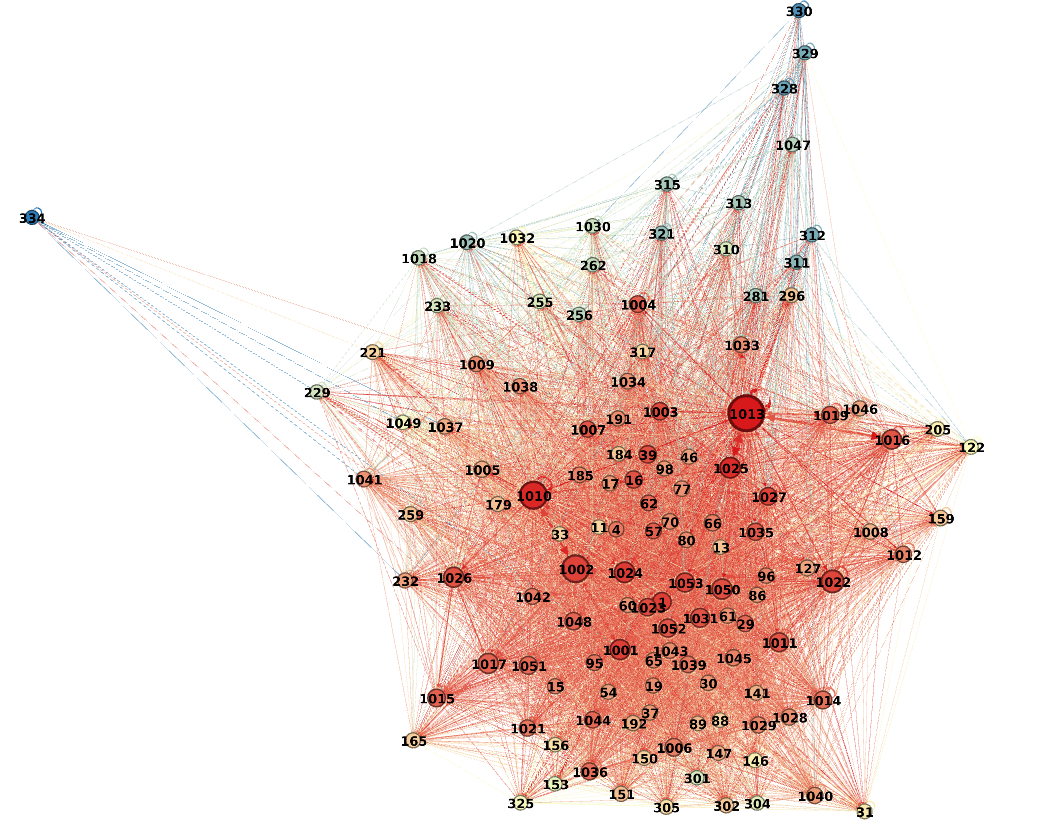
\includegraphics[width=14cm]{./pictures/M1_gephi.png}
	\end{center}
	\caption{M1 network}
	\label{fig:M1_gephi}
\end{figure}

The results of this new model - denoted from now on as M1 and ploted in figure \ref{fig:M1_gephi} - were more prominsing than the old produced by M0, but still failed to solve some critical issues of this peculiar graph.

\begin{itemize}
	\item The distribution of links among clusters and their dimensions is more homogeneous. Considering that the maximum number of links in a pre-clustering node is around 8000, the only clusters produced by M1 over 10000 links are 1013, 1010, 1002 and 1022 with outer link connections of 28637, 17865, 16277 and 10356 and sizes 23, 11, 5, 8. Besides the first cluster that seems to overaggregate the nodes of Central railway station with its dense neighbourhood, the other hubs have definitely a more reasonable dimension, consistent with the huge amount of trafic present in their locations, respectively Sempione Park, Cadorna and Via dei Mille. Moreover, in this new framework, the city center is much less aggregated and there are many additional clusters in periphery. However, the middle range zone represented by Garibaldi station is completely divided in singletons and also in general the number of isolated nodes is much larger than in M0 (74 nodes) with a total of 127 macro-nodes, only a half of the original dataset.
	
	\begin{figure}[H]
		\begin{subfigure}[H]{0.5\linewidth}
			\centering
			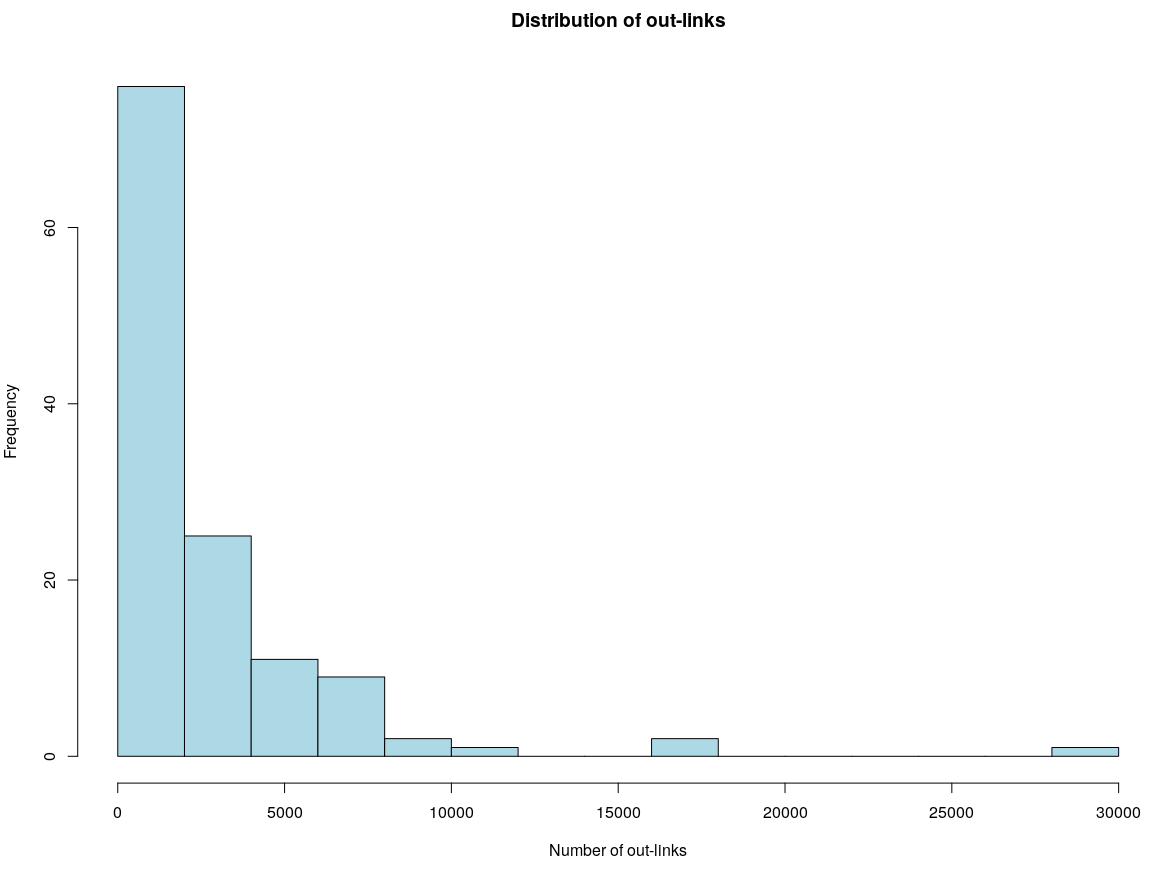
\includegraphics[width=70 mm]{pictures/M1_n_links.png}
			\caption{Distribution of links}
			\label{fig:M1_n_links}
		\end{subfigure}
		\hfill
		\begin{subfigure}[H]{0.5\linewidth}
			\centering
			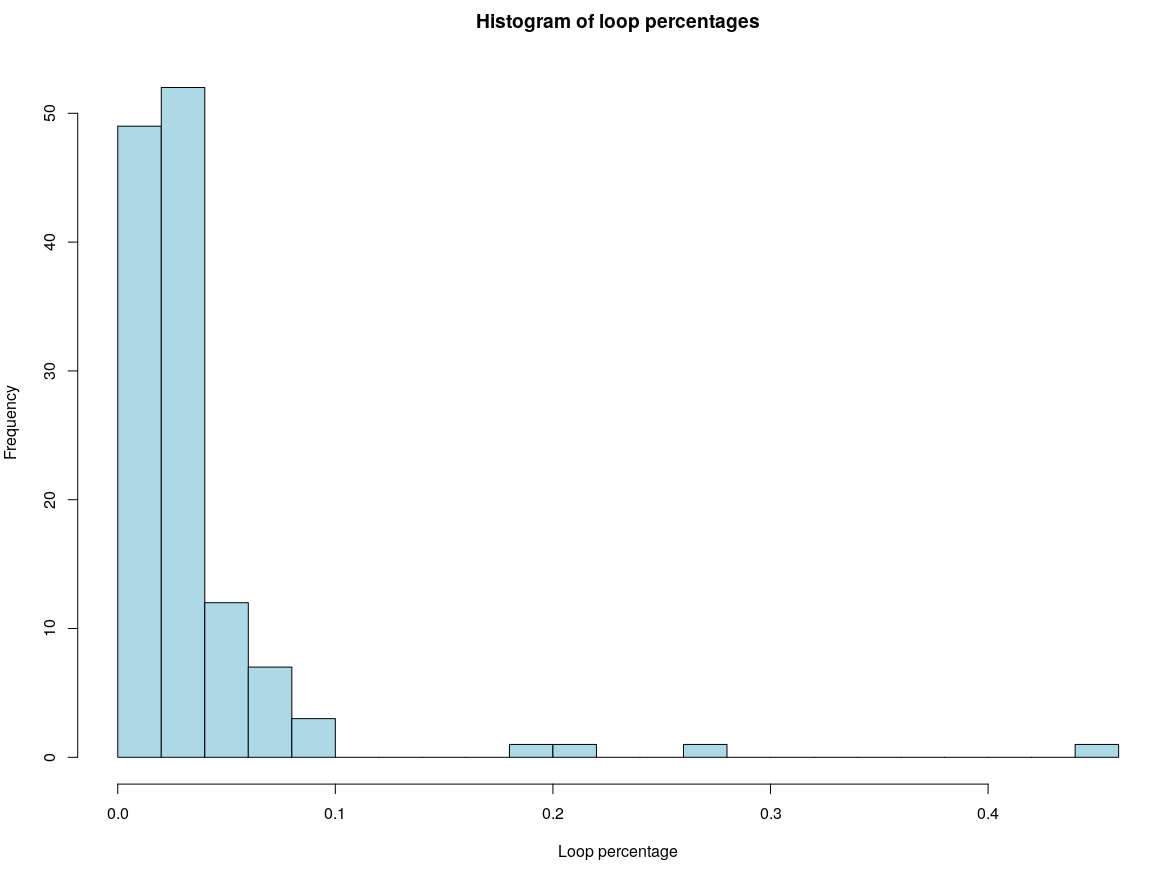
\includegraphics[width=70 mm]{pictures/M1_loop_percentages.png}
			\caption{Histogram of loop percentages}
			\label{fig:loop_distribution_M1}
		\end{subfigure}%
		\caption{Properties of M1}
	\end{figure}

	\item loop function: by construction model M1 has a very low number of loops, the weighted loop coefficient $ P_1=4.72\% $, denoting quite a good adhrence with the undelying net topology, in front of a $ G_1=3.56 $. The estimate is also quite robust with respect to the distribution of loops, seen in figure \ref{fig:loop_distribution_M1}, indeed there are only four outlier groups exceeding the safety threshold of 10\%: the usual unclusterized extreme nodes 330, 334 and clusters 1047, 1013. 1047 is a quite unusual in nature, since it is the most peripheric cluster created, so - also in in light of its negligible numeroussness, just 715 links - we can consider its behaviour as an outlier both irrelevant and somehow understandable. Central station, cluster 1013, on the other hand, is definitely the product of an extreme overaggregation due to the high proximity of business locations like Gioia and the Lombardy Region seat. Unfortunately this problem can't be solved with elementary tuning of the penalised-DBSCAN parameters, because this is an intrinsic frailty of the algorithm which is incapable of aggreating well zones which are very close together, still separate, but share a strong difference in density, like Garibaldi (left in singletons) and Central (too clusterized).

\end{itemize}

\subsection{Disaggregating improper clusters}
In order to improve the performance given by M1, a sensible subdivision of cluster 1013 seemed unavoidable. Indeed, as it had already been clarified, there were strong topological reasons to consider that merging improper and, as a final consideration, just notice that the contribution to the total weighted loop percentage $ P_1=4.72\% $ given only by 1013 was $ 1.54\% $. Almost $ 1/3 $ of the improper aggregation of the net was located in this single macro-cluster! Since $ P_{1013}^1=18.78\% $, a separation in 2 or 3 subsets seemed - a priori - to be the right choice. This intuition found confirmation in the results. Given $ \hat{\alpha}=0.8,\ \hat{\beta}=0,\ \hat{\gamma}=0.5 $ as in the previous subsection, we decided to tune locally the penalized DBSCAN, playing a bit with the value of $ \varepsilon $, restricted to the mere region 1013. Plots in figure \ref{fig:1013} show the variation in  nature and loop funtion of the cluster under increasing $ \varepsilon $. If the value is too small the nodes are almost all singletons, hence there are actually just a few loops. As $ \varepsilon $ increases, the aggregation starts to play a decisive role making the loop function rise quadratically. Taking into account that our goal was that of halving the loop percentage, appeared reasonable to select $\varepsilon =0.35$. Indeed, as a result, the aim was achieved using only two clusters which, from direct inspection, seemed quite reasonable: effectively creating a virtual barrier dividing Gioia-district from Central railway station.

\begin{figure}[H]
	\begin{subfigure}[H]{0.5\linewidth}
		\centering
		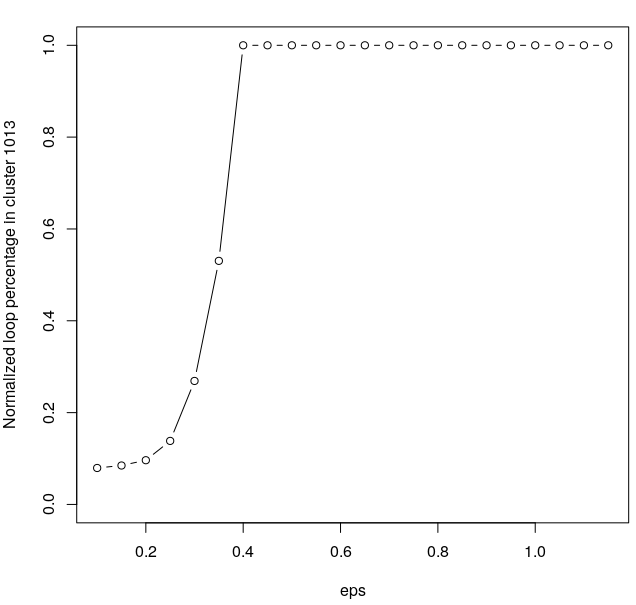
\includegraphics[width=70 mm]{pictures/1013_1.png}
		\caption{Normalized percentage of links}
	\end{subfigure}
	\hfill
	\begin{subfigure}[H]{0.54\linewidth}
		\centering
		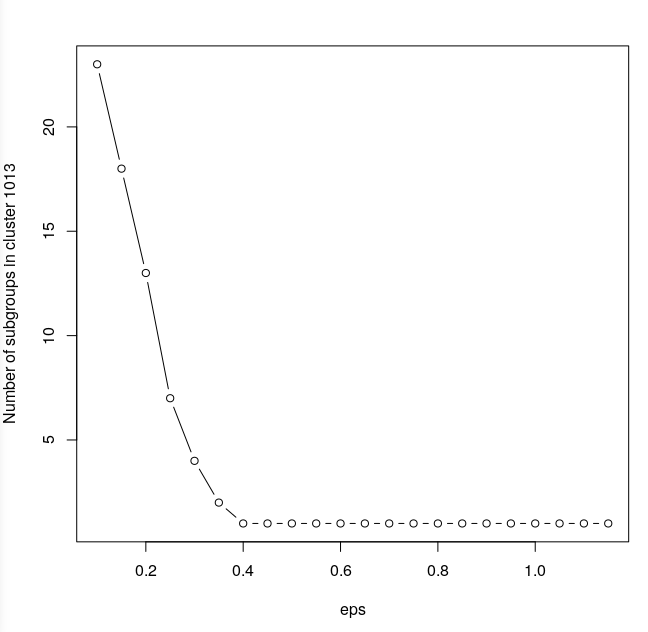
\includegraphics[width=70 mm]{pictures/1013_2.png}
		\caption{Number of sub-clusters}
	\end{subfigure}%
	\caption{Sub-custering of group 1013}
	\label{fig:1013}
\end{figure}
Calling the model disaggregating the macro-group as M2, we found a clusterization structure with only the $ 4\% $ of weighted loops and strongly topologically adherent with the original network. However, there were still two directions on which it could had been possible an improvement: the number of singletons was very high -  specifically in the zone where distances were a bit increased w.r.t the standard Euclidean ones -  and also the baricenters of many sets appeared often very closed to other singletons. We will discuss a possible solution to this problem in the next section.

\section{Iterated Penalized DBSCAN}
In order to force the aggregation of some more isolated point, reduce the computational complexity of the Bayesian study - that will be the main core of the project - and finally attain a more uniform spatial layout closer to Milan viability, we proposed one last modification to the already implemented corrected penalized DBSCAN M2. The main variation in model M3 - as will be denoted form now on - consisted in the addition of a second layer of penalized DBSCAN to the already proposed spatial grid. There are several reasons that make fruitful this choice, since dividing the clusterization in two phases partially resolves some problems of aggregation. Indeed, for instance, it allows to first compute the most interconnected sets and then substitute them with their ideal Euclidiean baricenters - a reasonable approximation of their penalized equivalents, for which lacks a rigorous definition, probably the minimum of some suitable optimization problem, to be solved with ad-hoc computationally intensive techniques. In particular, letting first layer clusters collapse on their baricenters somehow makes them "less attractive" for the second iteration; in the sense that, in principle, a reasonably large penalized neigbourhood without any station in proximity should be created around any of them, at least in case of proper clustering. Conversely, in case of missed points, the algorithm will tend to incorporate more easily the lost singletons in the area, thus stimulating the clusterization of the remaining units. See figure \ref{fig:comparison} for a comparison.
\begin{figure}[H]
	\begin{subfigure}[H]{0.5\linewidth}
		\centering
		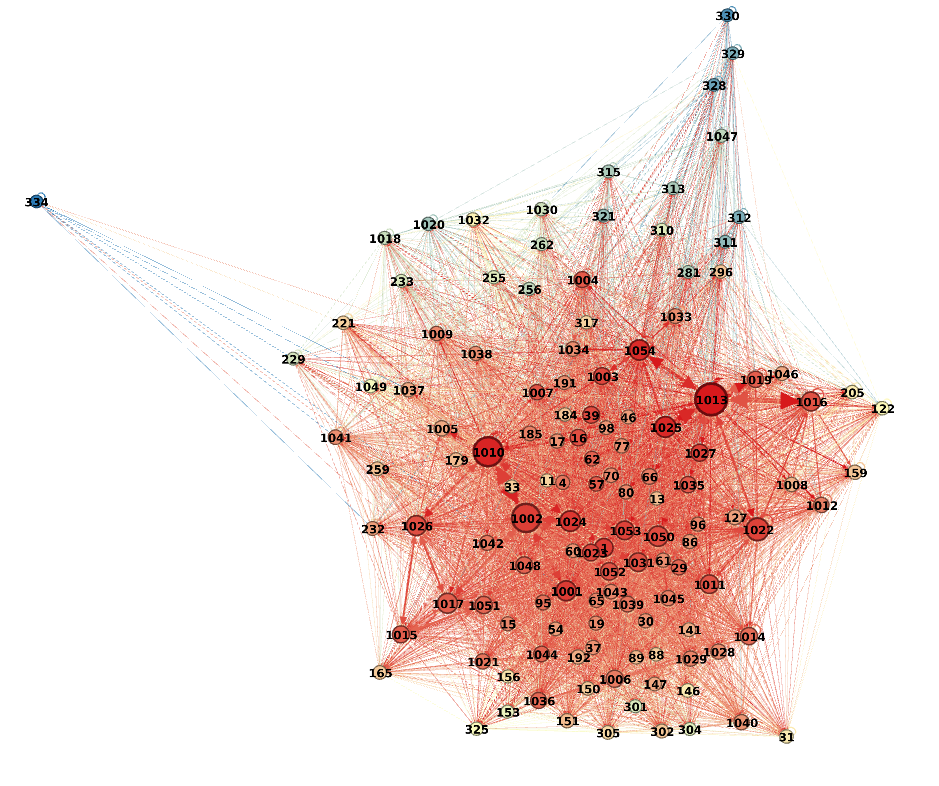
\includegraphics[width=133 mm]{pictures/M2_graph.png}
		\caption{Model M2}
	\end{subfigure}
	\vfill
	\begin{subfigure}[H]{0.5\linewidth}
		\centering
		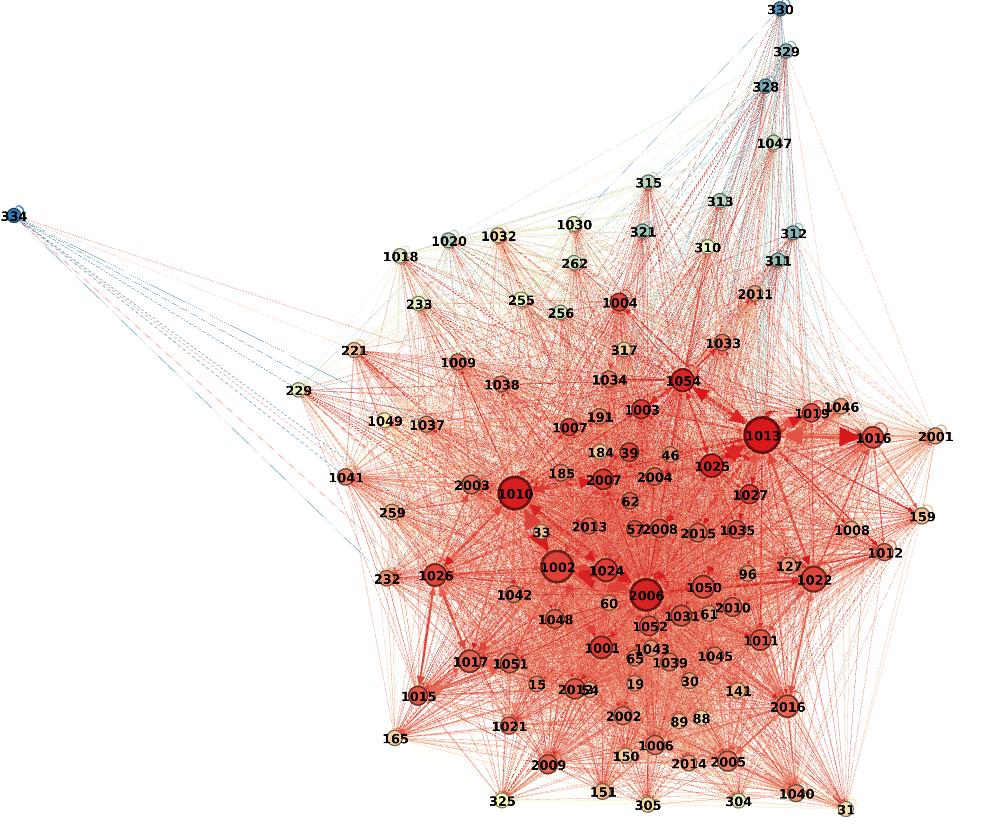
\includegraphics[width=133 mm]{pictures/M3_graph.png}
		\caption{Model M3}
	\end{subfigure}%
	\caption{Comparison between models}
	\label{fig:comparison}
\end{figure}

Besides visual inspection, there were several reasons for which M3 seemed to outclass its predecessor, but let us first give some details about the design of the second iteration of penalized DBSCAN. The procedure was exactly the same sequence of steps defined the previous case, with a strong difference: here $ \alpha,\ \beta,\ \gamma $ are fixed with the same values employed in M2, since - logically speaking - the topological parameters should be constant on a fixed network independently of the clustering, in absence of overaggregation. On the other hand, we left a bit of flexibility on $ \varepsilon $ making it vary in the same interval grid described in M1. We evaluated the most effective choice of $ \varepsilon $ still through the same $ GOF $ function and not surprisingly the minimum was found for $ \hat{\varepsilon}=1.10 $, very close to $ 1.15 $, the one selected by the first p-DBSCAN clusterization. One might ask itself if adding more iterations would not improve even further the aggregation. It depends, but in general no, since repeating too much the procedure may amplify the difference between penalised and Euclidean baricenters, originating improper overaggregation more frequently. In this particular case, even a third layer of clustering is not very effective, if not detrimental.

\subsection{Final results}
As a conclusion let us discuss the final results produced by M3 clustering. It's worth starting from the weighted loop percentage of the net, which has always been the simplest way to measure the goodness-of-fit of a clustering w.r.t. the true hidden topology. As already pointed out before, by hypothesis $ P_3\geq P_2 $. The issue lied in how great the difference was. Luckily a tolerable quantity: just $ 4.35\% $: starting from a benchmark of $ 3.99\% $; note this quantity to be still smaller than M1's average weighted loop percentage. Moreover, this estimate can also be considered quite robust, since the only outliers - i.e. stations over the $ 10\% $ in loop percentage - are the already well known extreme nodes 330, 334 and 1047, plus Central railway station cluster 1013, with a value of $ 10.53\% $, slightly out of the bounds, as seen in picture  figure \ref{fig:M3b}. In our personal opinion, this was enough evidence to believe this clusterization being able to capture with very small loss the actual graph structure, hence making a proper gathering of the nodes.\\
Another issue which had always been considered a clever way to avoid overaggregation was monitoring the inopportune presence of disporoportionate cluster sizes. Of course, since the topology under analysis was that of a circular metropolis, it seemed reasonable to expect a network whose distribution in the link number was approximating a power law. Therefore, it also appeared quite natural to forecast the presence of a few hubs whose size exceeded the standard dimension of other nodes. However, the theory wants these centers of interest to be in reduced number and possibly coherent with the scale of the problem. In our framework, we selected the threshold for having an hub at the usual $ 10000-12000 $ links which amounts to $ 2000 $ departures/week. The sole clusters able to surpass this limit were 1002 (Cadorna station), 1010 (Sempione), 1013 (Central station), 1022 (Viale Indipendenza-Via dei Mille), 2006 (Cordusio), details in figure \ref{fig:M3a}. However their loop percentages still looked under control: $ 1.3\%,\ 9.48\%,\ 10.53\%,\ 7.16\%,\ 2.9\% $. Motivated by these positive results, we decided to accept M3 as baseline for our future works.

\begin{figure}[H]
	\begin{subfigure}[H]{0.54\linewidth}
		\centering
		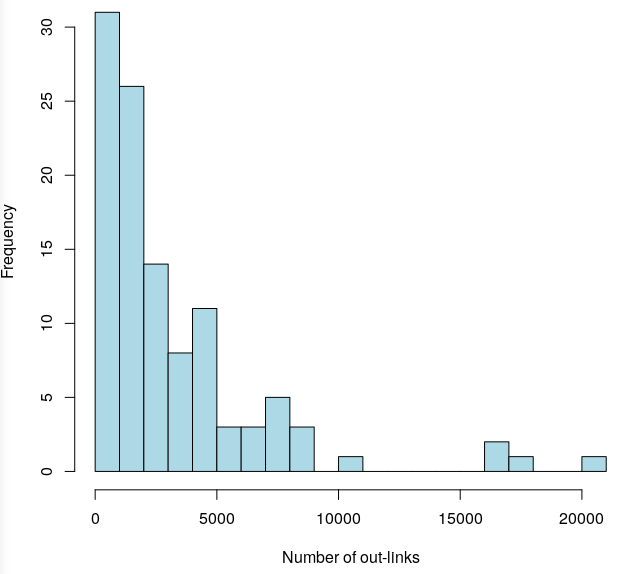
\includegraphics[width=58 mm]{pictures/M3_links.png}
		\caption{Number of departures per cluster}
		\label{fig:M3a}
	\end{subfigure}
	\hfill
		\begin{subfigure}[H]{0.50\linewidth}
		\centering
		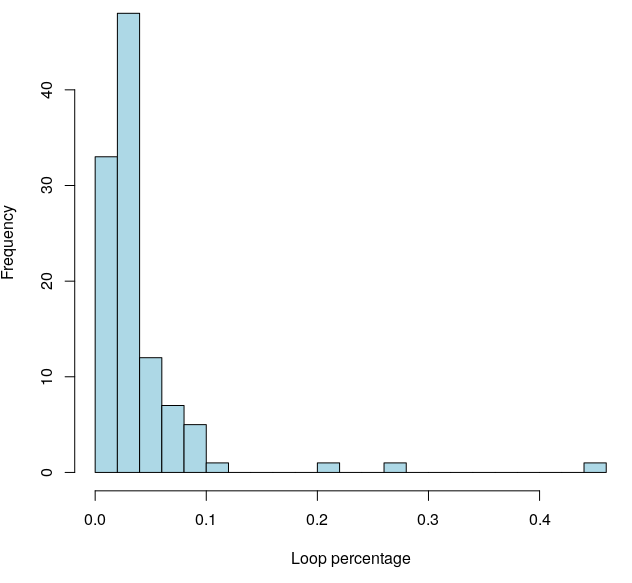
\includegraphics[width=58 mm]{pictures/M3_loop.png}
		\caption{Loop percentage distribution}
		\label{fig:M3b}
	\end{subfigure}%
	\caption{M3 results}
\end{figure}

\chapter{Frequentist preprocessing}
The main goal of this report is suggesting strategies to predict the traffic of the BikeMi network in Milan. In order to achieve this goal, we will follow two distinct, but complementary, paths: a global analysis whose main aim is finding a way to forecast the overall amount of trips that will be carried out during a well specified day, and a network analysis where we want to determine the global number of trips started or ended in the macro-nodes generated through the corrected DBSCAN preprocessing, that we have mentioned before. In both cases our main purpose is using models which are feasible enough from the computational viewpoint to allow, without a big loss in terms of precision, the realization of forecasts in a maximum time span of one day. In order to open the way for a Bayesian analysis, we decided first to perform a frequentist preprocessing. The goal was very simple: identify possible superstructures that have a Bayesian counterpart (like moving avarages and periods in BSTS), tackle the identification of suitable regressors and finally verify the stationarity of residuals according to these models. Conversely, the advantage of a Bayesian setting lied in the possibility to select and interpret in a more complete and effective way both uncertainty and errors, which are always protagonists in contexts where it is possible to determine posterior distributions of parameters.

\section{Data representation}
It is important to have immediately a grasp of the nature of data we are going to analyze: as it can be seen in picture, we are dealing with counts that even between the most relevant stations are null almost every time. This induces necessarily the need to clusterize through corrected DBSCAN multiple stations.

\begin{figure}[H]
	\centering
	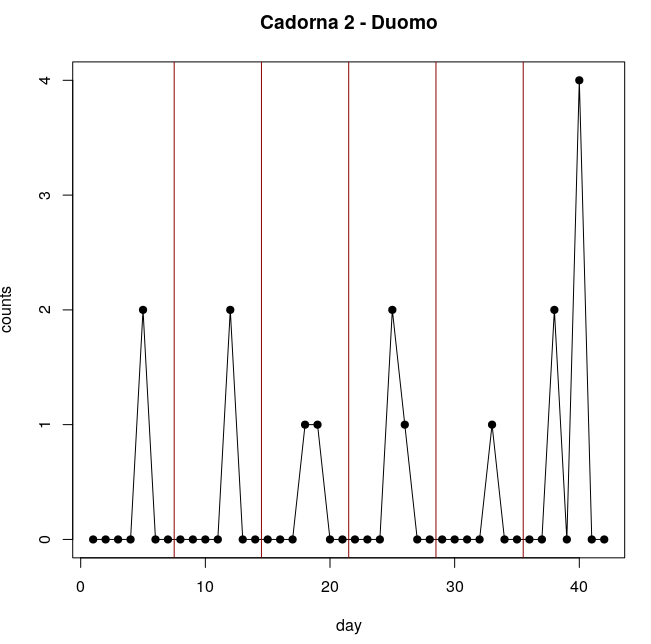
\includegraphics[width=85 mm]{pictures/cadorna_duomo.png}
	\label{fig:cadorna_duomo}
	\caption{Traffic from Cadorna main park and Duomo stations}
\end{figure}

Since dealing with a problem of traffic concerning light vehicles, atmospherical conditions have been examined in order to find some interplay with the variation in the number of bikes on the net. In the following graph, we show a qualitative comparison in the effect of rain, wind, humidity and temperature with the overall amount of bikes in a day. Unfortunatey, the data available for $ 2016 $ share a daily horizon, thus we can't have a precise division in time slots for a more refined type of analyis. Nonetheless, we will try to disagregate the study also in time zones, struggling to capture the discrepancies in volume through other strategies typical of structural time series.

\begin{figure}[H]
	\begin{subfigure}[H]{1\linewidth}
		\centering
		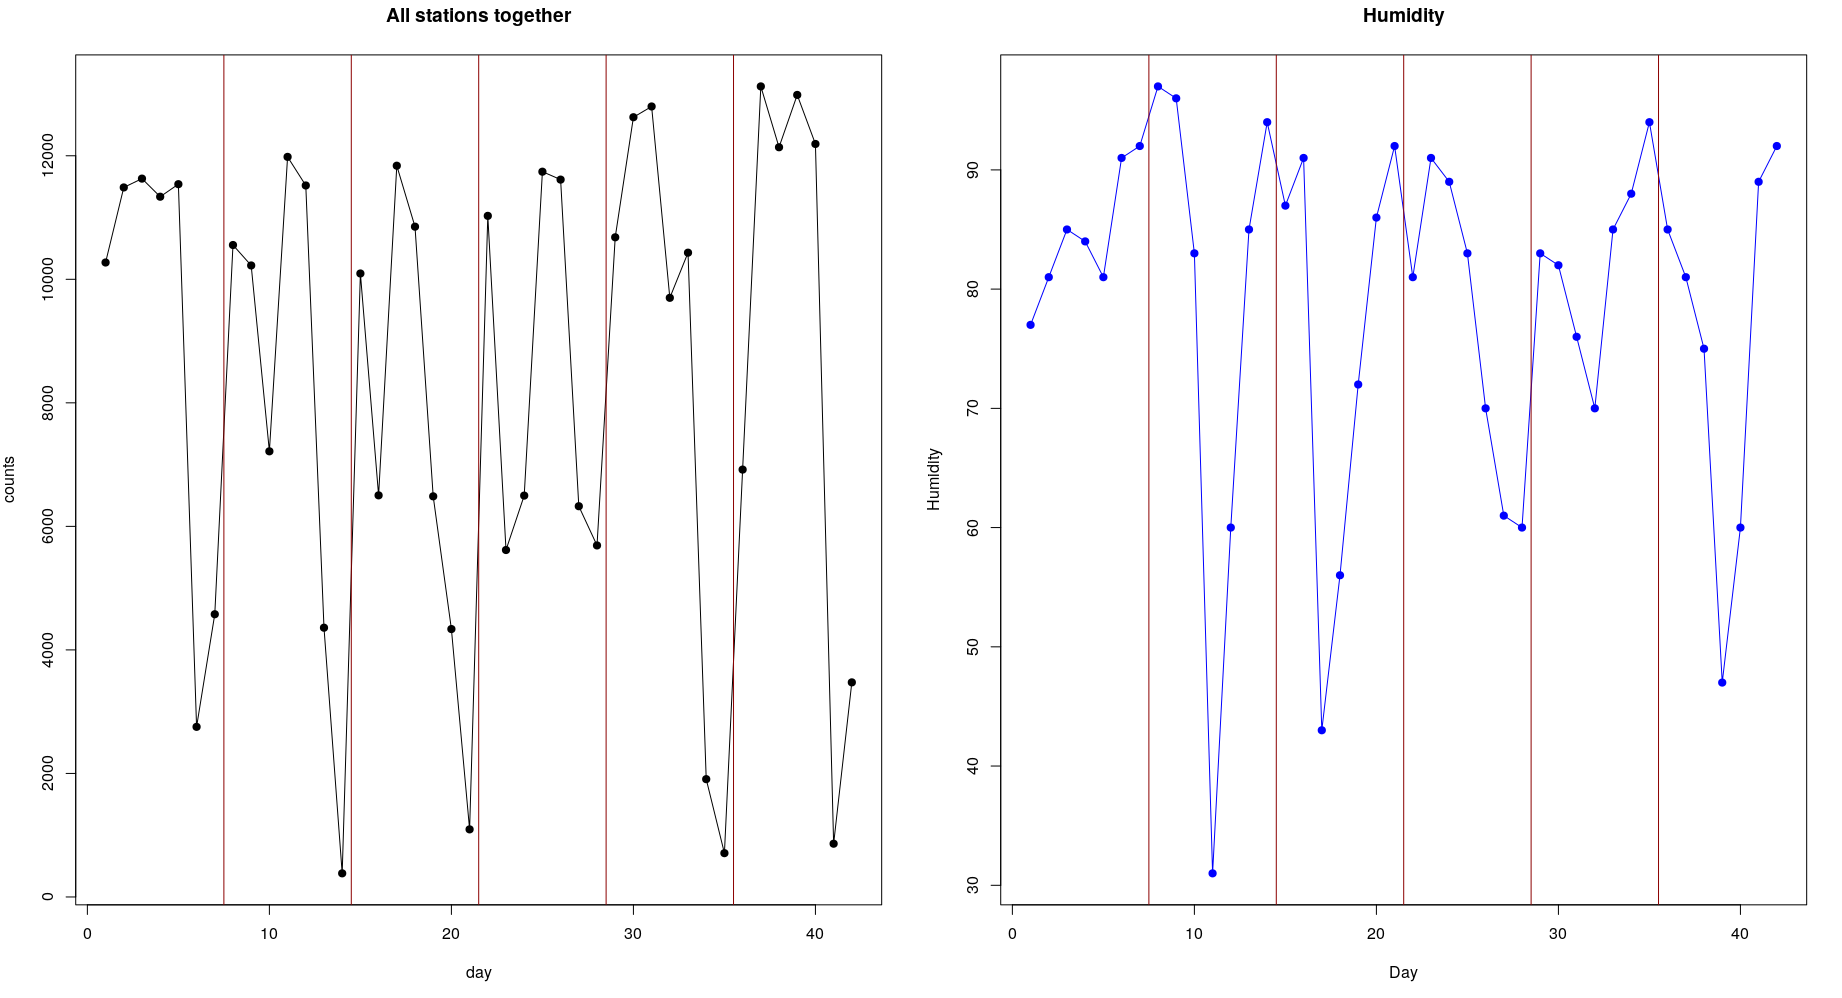
\includegraphics[width=110 mm]{pictures/humidity.png}
		\caption{Humidity}
		\label{fig:humidity}
	\end{subfigure}
	\vfill
	\begin{subfigure}[H]{1\linewidth}
		\centering
		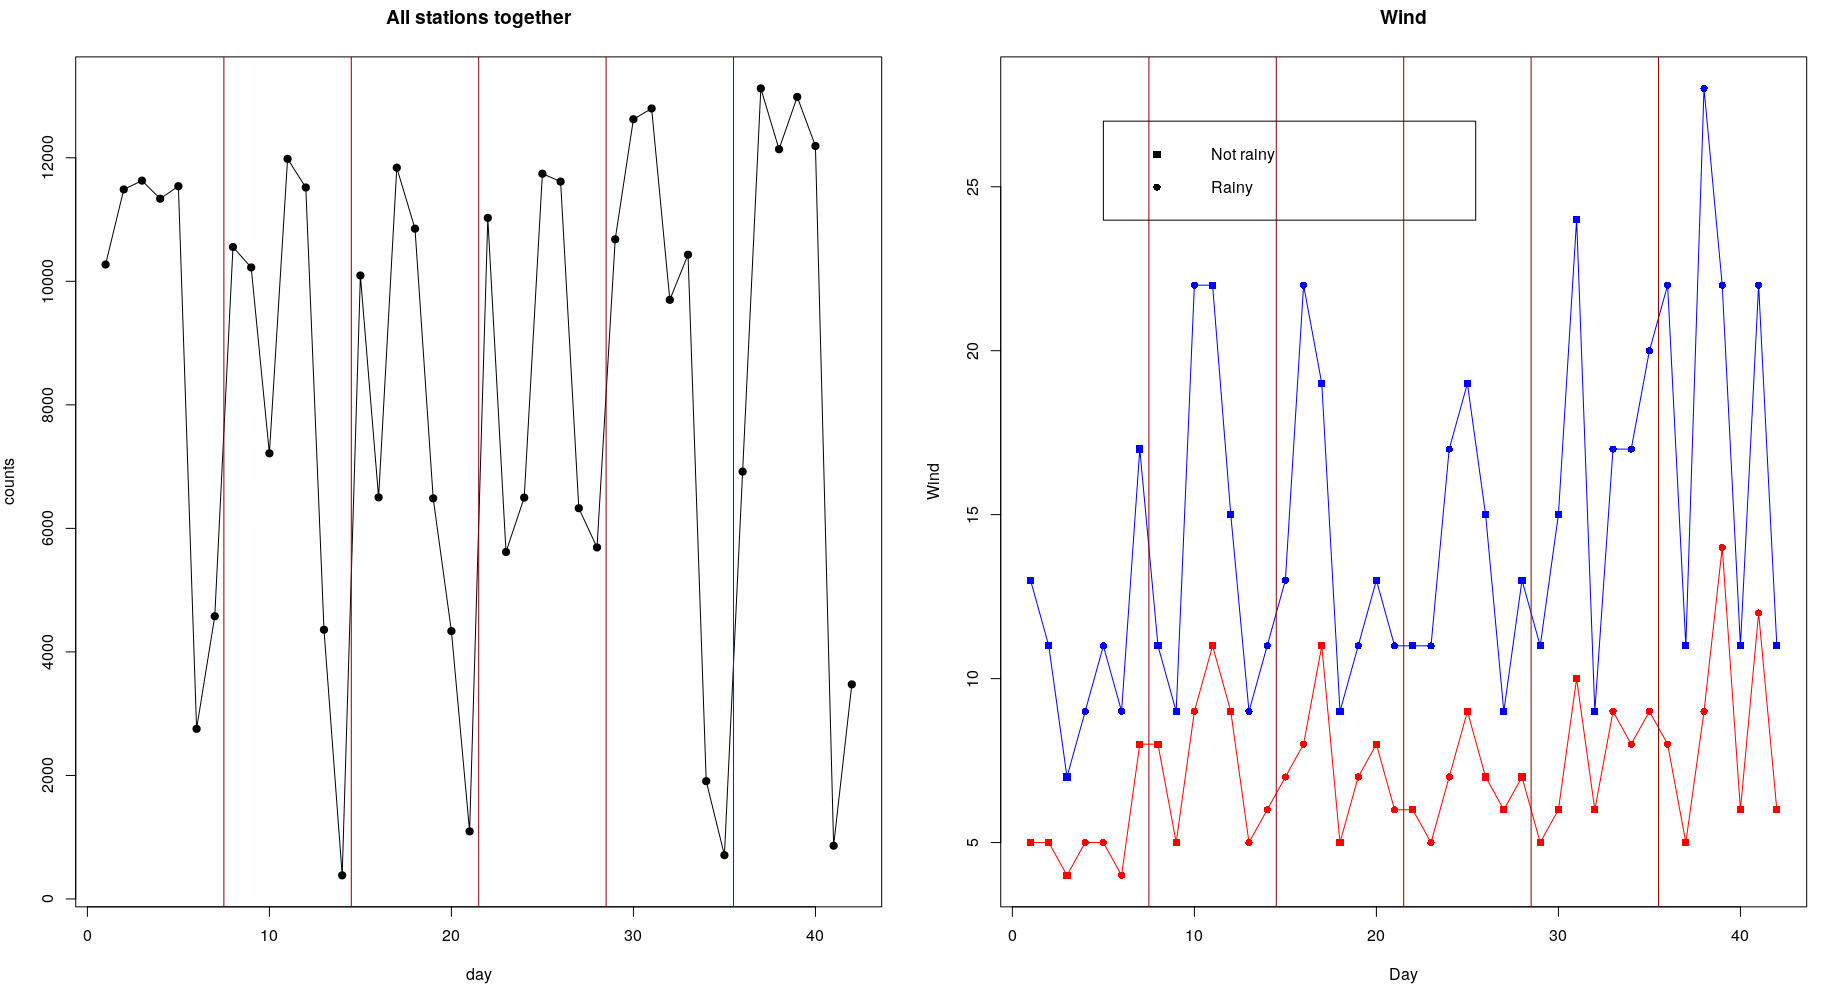
\includegraphics[width=110 mm]{pictures/wind.png}
		\caption{Wind}
		\label{fig:wind}
	\end{subfigure}
	\vfill
	\begin{subfigure}[H]{1\linewidth}
		\centering
		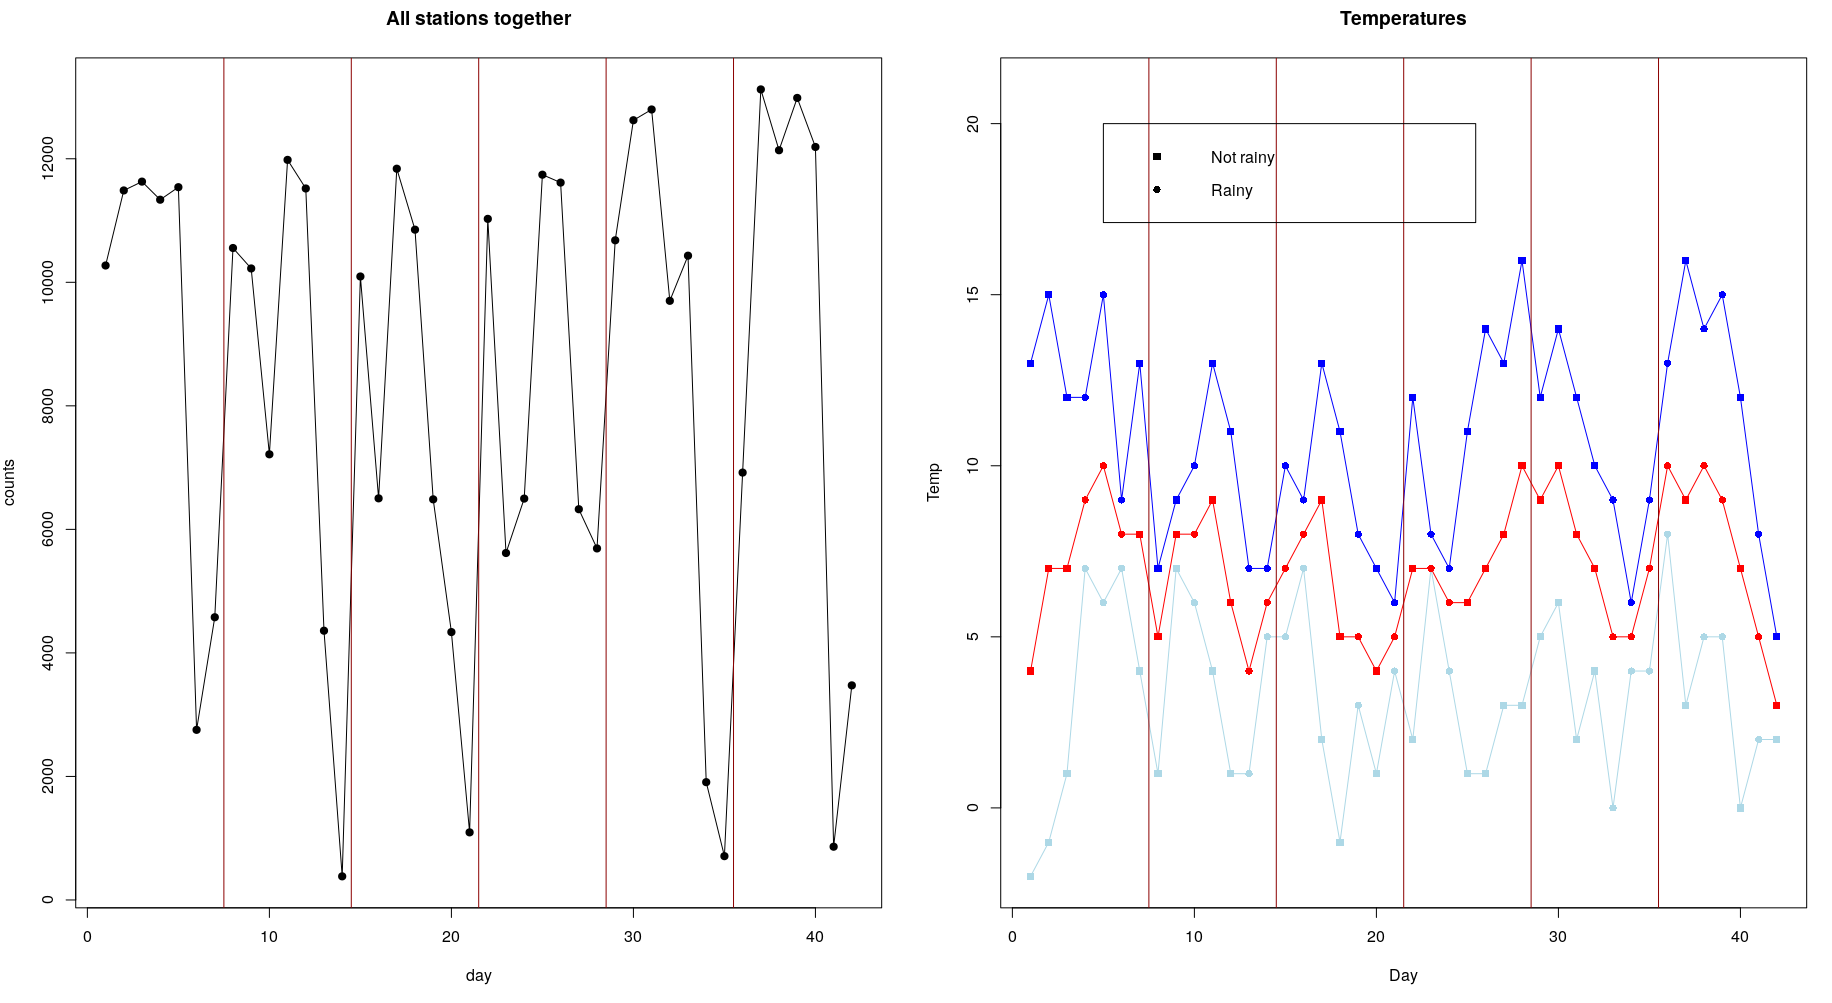
\includegraphics[width=110 mm]{pictures/temperatures.png}
		\caption{Temperatures}
		\label{fig:temperature}
	\end{subfigure}
	\caption{Action of atmospheric conditions vs total traffic}
\end{figure}
\newpage

As for the moment just observe that there does not appear to be a strong relationship between traffic and humidity or wind, while on the opposite temperature seems sometimes proportional to the effective output. A bit different is the nature of rain. Even though the time series seems to have a natural periodicity, the action of rain sometimes disrupts this behaviour, since the number of bikes drops abruptly in correspondence of strong phenmena.  This easily meets intuition: in a big metropolis like Milan the action of wind and humidity is mitigated by artificial warming and the vertical structure of the city. Viceversa, rain can be considered the universal strongest bollard against the usage of bikes, at least neglecting competitive users or orthodox environmentalists. Motivated by these results, we will try to use the two factors as predictive tools in the future.

\section{Stationarization}
In order to check the possibility to consider our model as a structural time series, we decided to employ a frequentist moving average + periodicity filtering, a second goal will be that of verifying the stationarity of the found residuals. The idea behind the stationarization is substantially the following: each datum can be seen as the sum of a trend represented by a moving average, a periodic component repeating itself identical during the various weeks and a residual effect: in principle a stationary process (for instance a white noise or an ARMAX paradigm): $ y_t = m_t + s_t +r_t $ where $ m $ is the m.a., $ s $ period and $ r $ residual. To produce these estimates we employed the following pre-codified techniques, described for instance in BD02, see bibliography.\\

\begin{algorithm}[H]
	\SetAlgoLined
	Set the time horizon T and period S;\\
	Set $ q=(S-1)/2 $;\\
	\For{$ i \in $ 1\ :\ T}
	{
		Compute $ m_i $ = $\sum_{j=\max\{-q,0\}}^{\min\{q,T\}} y_{i+j}/S$;
	}
	\For{$ k \in $ 1\ :\ S}
	{
		Compute the average $ w_k $ of the deviations $ \{(y_{k+jS} - m_{k+jS} ),\ q < k+jS \leq T-q\} $;
	}
	\For{$ t \in $ 1\ :\ T}
	{
		Compute  $ s_t = s_{k(t)} = w_k-S^{-1}\sum_{i=1}^{S}w_i $;\\
		Compute  $ r_t=y_t-m_t-s_t $;
	}

	\KwResult{Decomposition $ y_t=m_t+s_t+r_t $}
	\caption{Frequentist stationarization}
	
\end{algorithm}

\begin{figure}[H]
	\begin{subfigure}[H]{0.5\linewidth}
		\centering
		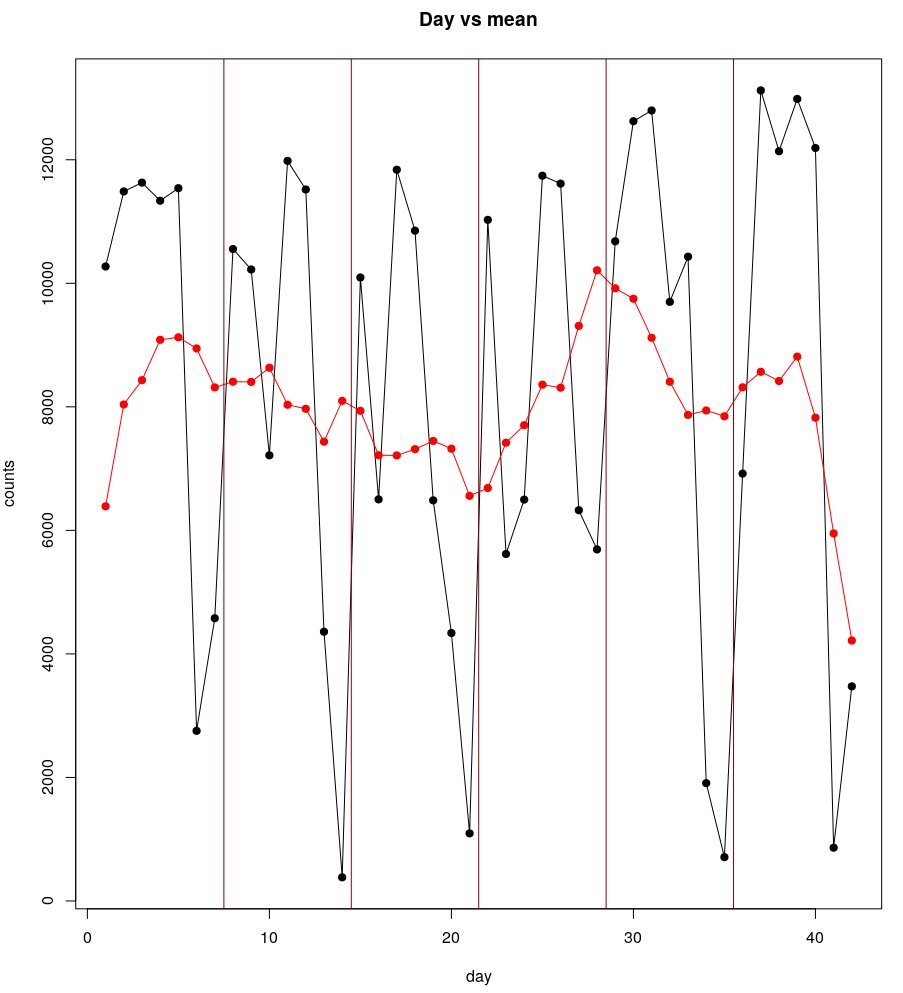
\includegraphics[width=65 mm]{pictures/moving_average.png}
		\caption{Moving average}
		\label{fig:ma}
	\end{subfigure}
	\hfill
	\begin{subfigure}[H]{0.5\linewidth}
		\centering
		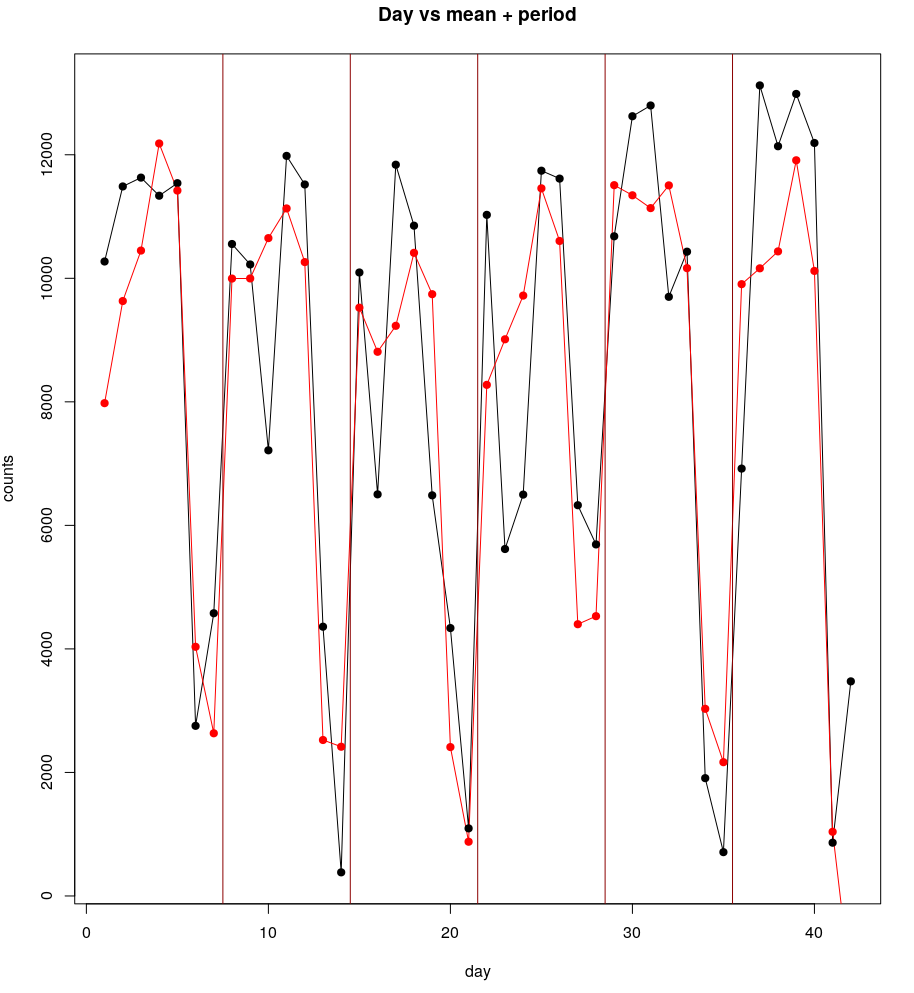
\includegraphics[width=65 mm]{pictures/period.png}
		\caption{Moving average + periodicity}
		\label{fig:period}
	\end{subfigure}
\end{figure}

Note that, apart from the irregularities deriving from the boundaries of the time span where the moving average works not properly well (i.e. the first and last weeks), all the other days show a quite regular trend and the $ m_t+s_t $ term captures already rather well the value of $ y_t $. Just observe also that most of the discrepancies emerge facing rainy days in which there are sudden variations (usually strong falls) with respect to standard behaviour of the historical series. This is a indirect sign of the need of a regression coefficent in the representation taking into account the role of weather. Indeed looking also at the residuals in figure \ref{fig:res}, we can see a good oscillating trend mostly negative in rainy days and positive in sunny ones. Moreover, the autocorrelation plot testifies that the residual chain has a white noise $ WN $ behavior, for this reason in BSTS models we will only consider the presence of an $ AR(1) $ effect or none at all, to be summed to the classic trend + periodicity baseline. According to most reliable frequentist stationarity tests (Augmented Dickey-Fuller, Phillips-Perron, KPSS) the p-value of having a non stationary chain is less than $ 0.10 $, hence we can quite confidently reject the null hypothesis and postulate the stationarity of the residuals of the chain.

\begin{figure}[H]
	\begin{subfigure}[H]{0.5\linewidth}
		\centering
		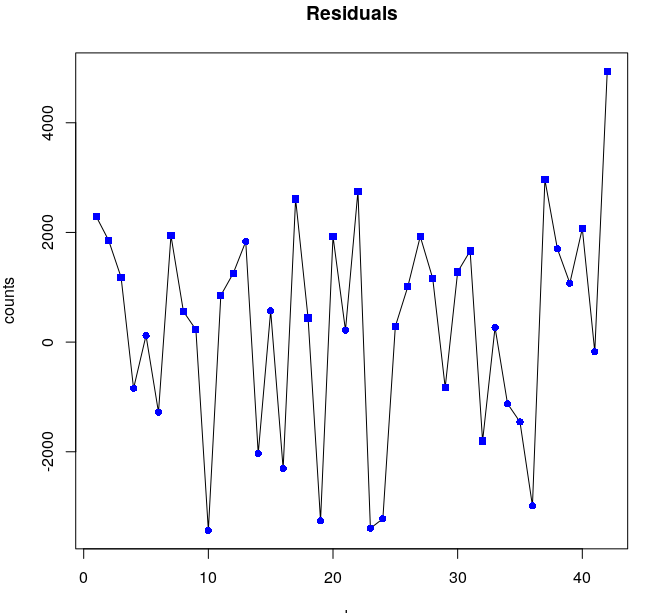
\includegraphics[width=65 mm]{pictures/residuals.png}
		\caption{Plot of the residuals with respect to weather}
	\end{subfigure}
	\hfill
	\begin{subfigure}[H]{0.5\linewidth}
		\centering
		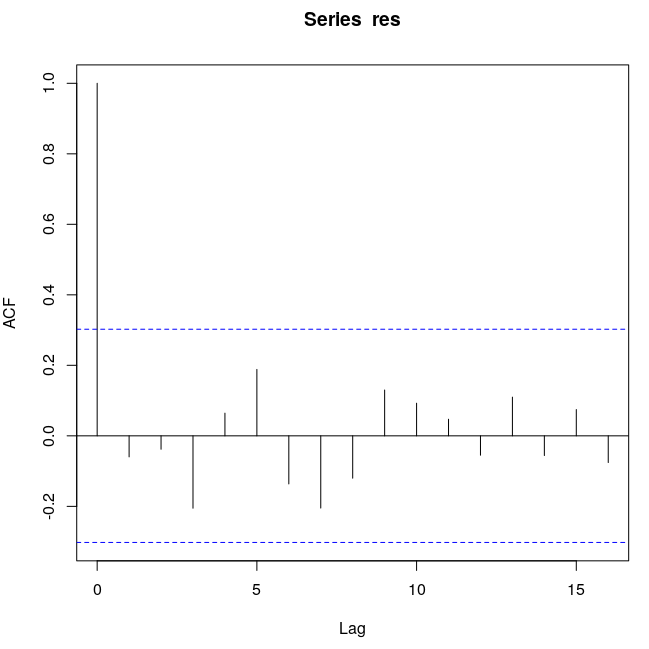
\includegraphics[width=65 mm]{pictures/corr.png}
		\caption{Autocorrelation plot of the residuals}
	\end{subfigure}
	\caption{Residuals}
		\label{fig:res}
\end{figure}

As a final comment before passing directly to the discussion of the models, let us just tackle the problem of subdivision in time zones. As mentioned before one of the main goals of our analyis is the ability to predict the number of bikes arriving or departing from a station at a certain hour. Obviously, with the data at our disposal, it is quite impossible to think at an hour to hour prediction. Anyway, a possible key to solve the infeasibility can be that of grouping together hours identifying precise behaviours. For instance if we want to summarize tha day in just four time slots we can consider the morning where people go to work (6 a.m. - 9 a.m.), the central hours (10 a.m. - 3 p.m), the late afternoon where people go back from work (4 p.m. - 7 p.m.) and finally the late evening (8 p.m. - 1 a.m.). Note that we don't have trips outside these time slots. Even though this division might appear trivial, is also very intuitive and balanced, since the volumes of traffic are almost the same in each of these zones (but the evening that for obvious reasons presents less movement than daily hours). Moreover we can see, specially looking at figure \ref{fig:tz} a sort of repeated periocity internal to the zones, ovelapping with the daily one already discovered through the previous algorithm. This superposition of a global period and an inner cycle will be the base from which to derive BSTS structures for time zones in the following chapter. Finally, observe that the effect of rain appears very dramatic also in this context, thus giving us a final corroboration of the need to add it to the set of covariates in any paradigm developed from now on.


\newpage
\begin{figure}[H]
	\centering
	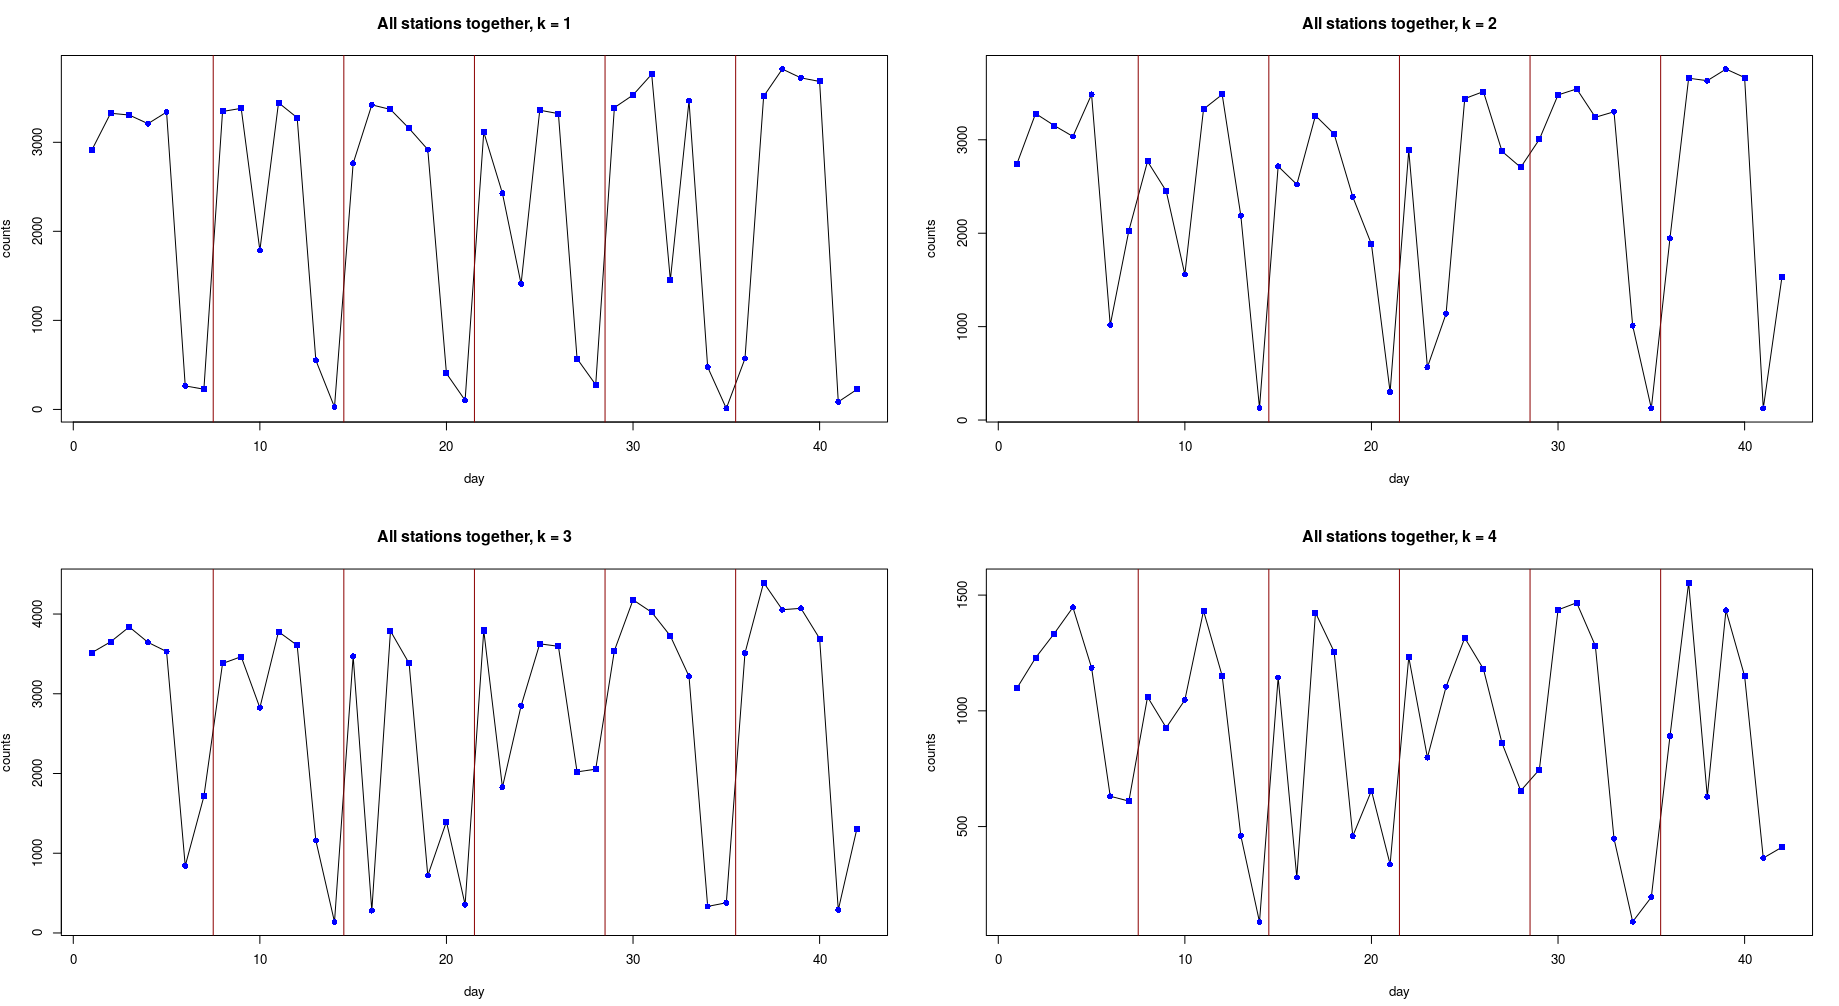
\includegraphics[width=160 mm]{pictures/division.png}
	\caption{Division in 4 time zones}
	\label{fig:tz}
\end{figure}

To conclude, notice that so far we have only mentioned the overall flow and not its entering/exiting distribution across time phases. We can get a grasp of the problem with picture \ref{fig:cp}. Indeed, there are some time slots with a lot of bikes exiting from the station (morning, black), while in other periods the same bikes seem to get back inside the same installations (afternoon, green, with high volume of traffic and night, blue, with less trips). This regularity somehow endorses an idea of periodic movement in bikers behaviour, that - for some reason, not necessarily due to work, since the division weekend-weekday seems not to affect too much the separation - use the device and later return exatly to the same place where they started, but in  different time phase. However, it's worth noting that this behaviour only affects the morning w.r.t evening and night. Indeed the afternoon period (in red), is quite stable and independet of the other two.

\begin{figure}[H]
	\centering
	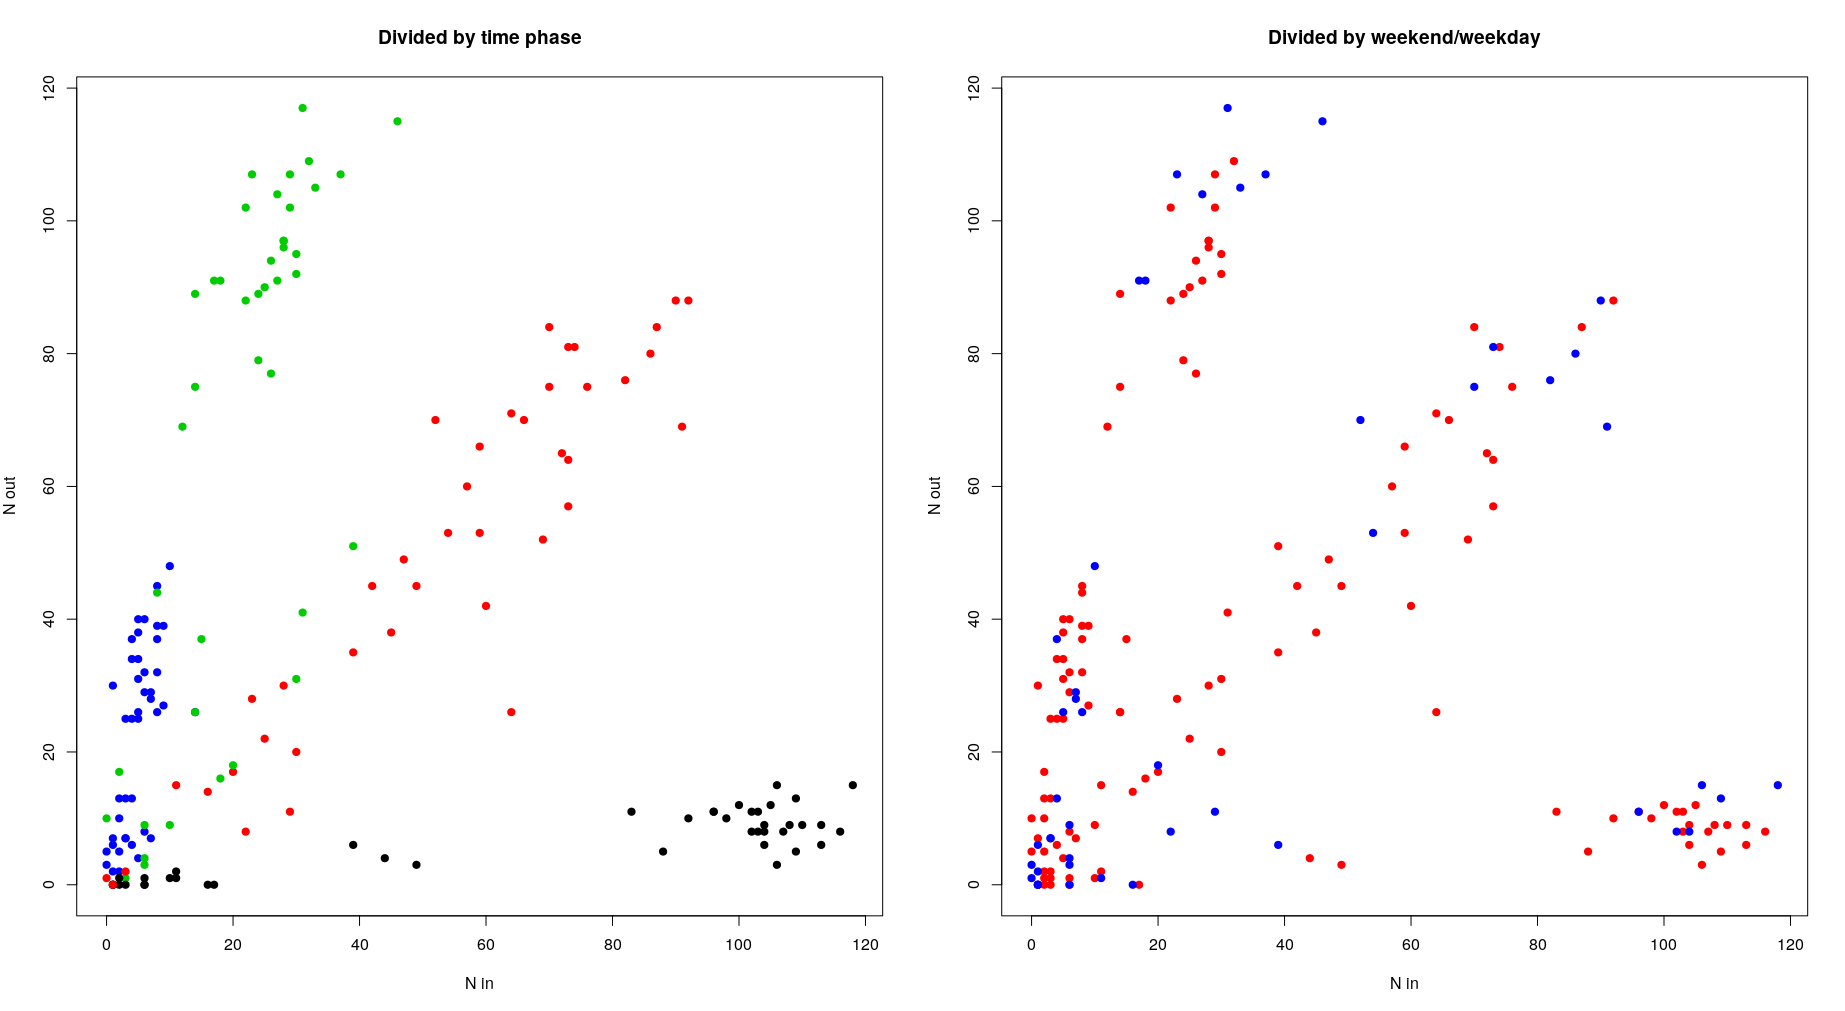
\includegraphics[width=150 mm]{pictures/correlation_color.png}
	\caption{Correlation of the different trips}
	\label{fig:cp}
\end{figure}

\chapter{Global model}
This chapter will be entirely devoted to the description and comparison among several possible Bayesian models, capable of sinthesizing the total taffic taking place in Milan during a six week long time span occured between January $ 25^{th} $ and March $ 6^{th} $, 2016. The total amount of data available to us consisted of 350,093 trips among stations of the BikeMi network. However, at least for this first part, we will only rely on the day-by-day cumulative traffic, neglecting the graph-specific topology. For further details about the dataset and atemporal analysis please refer to BG19 in the bibliography.\\
\\
Let us just point out the lineup of this chapter before entering into the heart of the modelistic phase: first we will discuss a loglinear strategy to deal with counting data, trying to highlight its usefulness in  covariate selection, but also the limits faced against heterogeneous and highly variable phenomena. Afterwards, we will devote some time discussing multiple Bayesian Structural Time Series approaches, eventually comparing the results with the ones produced by the aforementioned methods.

\section{Loglinear regression}
\subsection{Poisson likelihood}
The most straightforward model for counting data we considered is a loglinear generalized linear model, with Poisson likelihood :
\begin{model} Loglinear GLM with Poisson likelihood\\
	\begin{equation*}
	\begin{aligned}
	&\textsc{Model}\\
	&Y_t  |  \lambda_t \overset{\independent}{\sim} Pois(\lambda_t)\\
	&\log{\lambda_t} = \boldsymbol{\beta}^T\mathbf{z}_t\\
	\end{aligned}
	\qquad \qquad
	\begin{aligned}[c]
	&\textsc{Priors}\\
	&\boldsymbol{\beta} \sim \mathcal{N}_p(\mathbf{0}, \tau \mathbf{I})
	\end{aligned}
	\end{equation*}
\end{model}
Note that from now on normal distributios will be written using precisions. In this first version, moreover, $ \tau=0.001 $ and we take the following covariates:
\begin{itemize}
	\item $Y_{yest}$: volume of traffic during the previous day,
	\item $Y_{an}$: volume of traffic during the same day of the previous week,
	\item $W$: a binary variable representing weekdays or weekends, 
	\item $R_t$: a discrete variable representing the intensity of the rain (from 0 to 9),
	\item $R_{yest}$: analogous to $R_t$ referring to the previous day,
	\item $T$: the mean temperature of the day.
\end{itemize}  

We actually introduced two regression parameters for explaining the effect of $Y_{yest}$: we believe its effect on the next day can depend on the fact that we are on the weekends-weekdays boundary.   
The model is built on 35 observations, as the first week is used for defining the covariates. Results are not good at all, in terms of prediction of the already observed 35 days.\\
\\
Indeed, looking at the 90$\%$ credibility intervals for the $Y_t$ samples for the 35 days, we highlight that these intervals are shorter than what we need: the phenomenon is much more uncertain than what our model is able to describe.
Only 2 observations out of 35 fall inside the credibility intervals.
Having a look also at the distributions of regression parameters, we note that some covariates are irrelevant.
\begin{figure}[H]
	\centering
	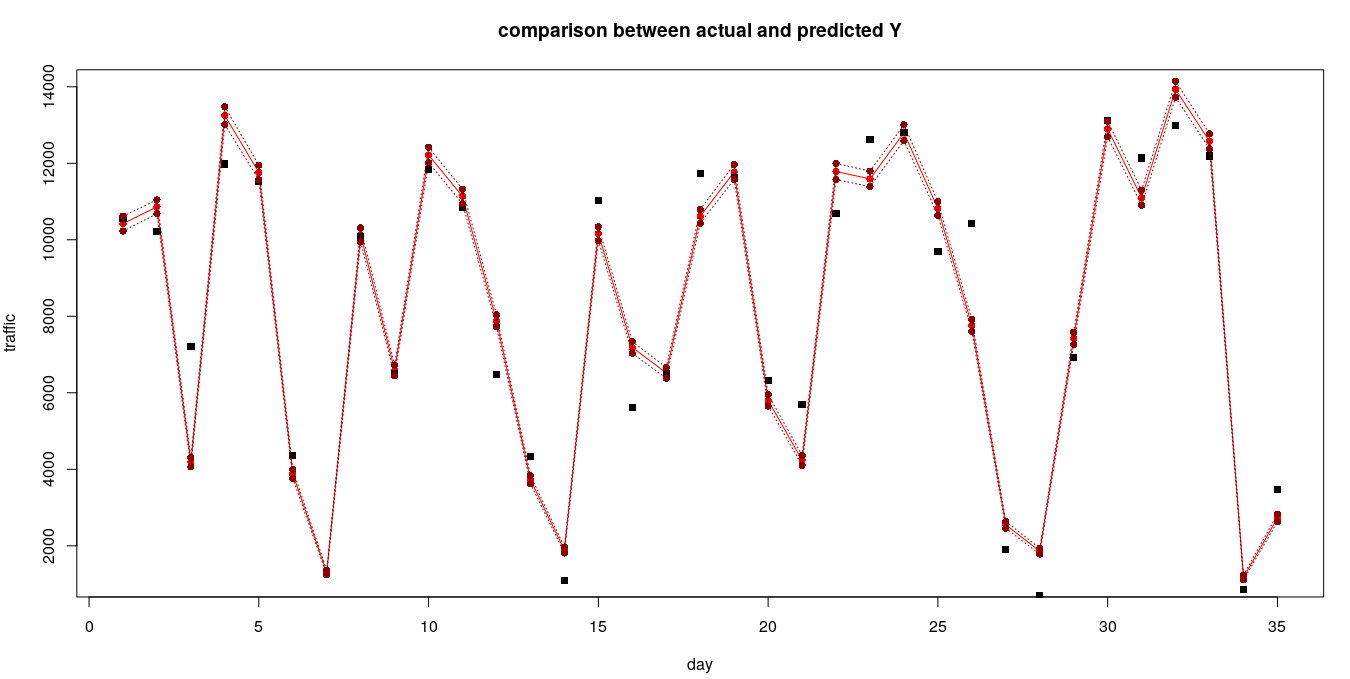
\includegraphics[width=160 mm]{pictures/poiss_y.png}
	\caption{90$\%$ Credibility intervals for $Y_t$ samples}
	\label{fig:poiss}
\end{figure}
Therefore, we tried a Spike\&Slab approach which suggests to remove $Y_{an}$, so we also have a similar model without that covariate. The results, as expected, are similar: the model still suffers the under-estimation of the phenomenon variability. For the previous considerations, we left the Poisson likelihood behind, without further investigating the role of covariates. However, from this initial model we extracted some useful information about the importance of specific variables in explaining the phenomenon: $W$, $R_T$ and $T$ appear influential covariates, and this is coherent with their model-related interpretation.

\begin{figure}[H]
	\centering
	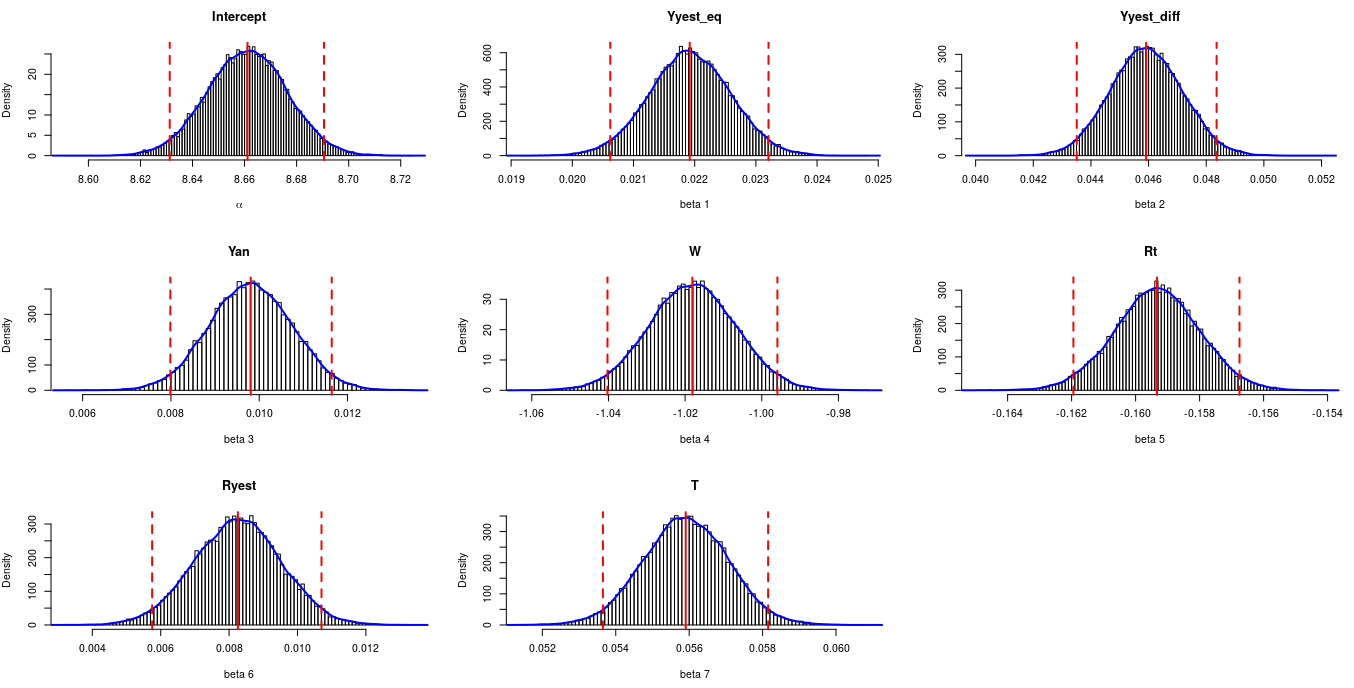
\includegraphics[width=160 mm]{pictures/poiss_beta.png}
	\caption{Distribution of regression parameters}
	\label{fig:poiss_beta}
\end{figure}
\subsection{Negative Binomial likelihood}
We needed to overcome the limits of the Poisson likelihood: those problems are related to the presence of a single parameter which determines both mean and variance, and to the fact that our phenomenon is intrinsically more uncertain than the Poisson model is able to describe. Following these observations, we proposed a loglinear generalized linear model with Negative Binomial likelihood. This distribution is described by two parameters, allowing for more flexibility; moreover it comes with an higher variance than its mean, and this could be what we needed.
We refer to the following formulation for the negative binomial density function:
\begin{equation}
f(k;r,p) = \frac{\Gamma(k+r)}{k!\ \Gamma(r)} p^k (1-p)^r \ \ \forall k\in\mathbb{N}
\end{equation}
According to this convention, if $X \sim NegBin(r,p)$, we have $\mathbb{E}[X] = \mu = \frac{r(1-p)}{p}$ and $Var[X] = \frac{r(1-p)}{p^2}$. Please, note that $p = \frac{r}{r+\mu}$. Jags implements this formulation.\\
We propose the following model: 
\begin{model} Loglinear GLM with Negative Binomial likelihood\\
	\begin{equation*}
	\begin{aligned}
	&\textsc{Model}\\
	&Y_t  |  p_t,r \overset{\independent}{\sim} NegBin(p_t,r)\\
	&p_t = \frac{r}{r+\mu_t}\\
	&\log{\mu_t} = \boldsymbol{\beta}^T\mathbf{z}_t\\
	\end{aligned}
	\qquad \qquad
	\begin{aligned}[c]
	&\textsc{Priors}\\
	&\boldsymbol{\beta} \sim \mathcal{N}_p(\mathbf{0}, 0.001\mathbf{I})\\
	&r \sim \mathcal{U}(0,50)\\
	&\\
	&\\
	\end{aligned}
	\end{equation*}
\end{model}
We selected a subset of covariates, basing our choice on both interpretation and hints from the Poisson model. We consider: $W$, 1 if weekend, 0 if weekday, $R_{t}^{class}$, discrete variable quantifying the intensity of the rain (from 0 to 9), $T$ mean temperature of the day. The regression tries to explain the mean value of the phenomenon, similarly to the Poisson model. Moreover, we let the $r$ parameter work in order to better fit the variability. We performed the simulation in Jags, and the properties of stationarity and requirements on autocorrelation are both easily satisfied. We show some of these plots:
\begin{figure}[H]
	\centering
	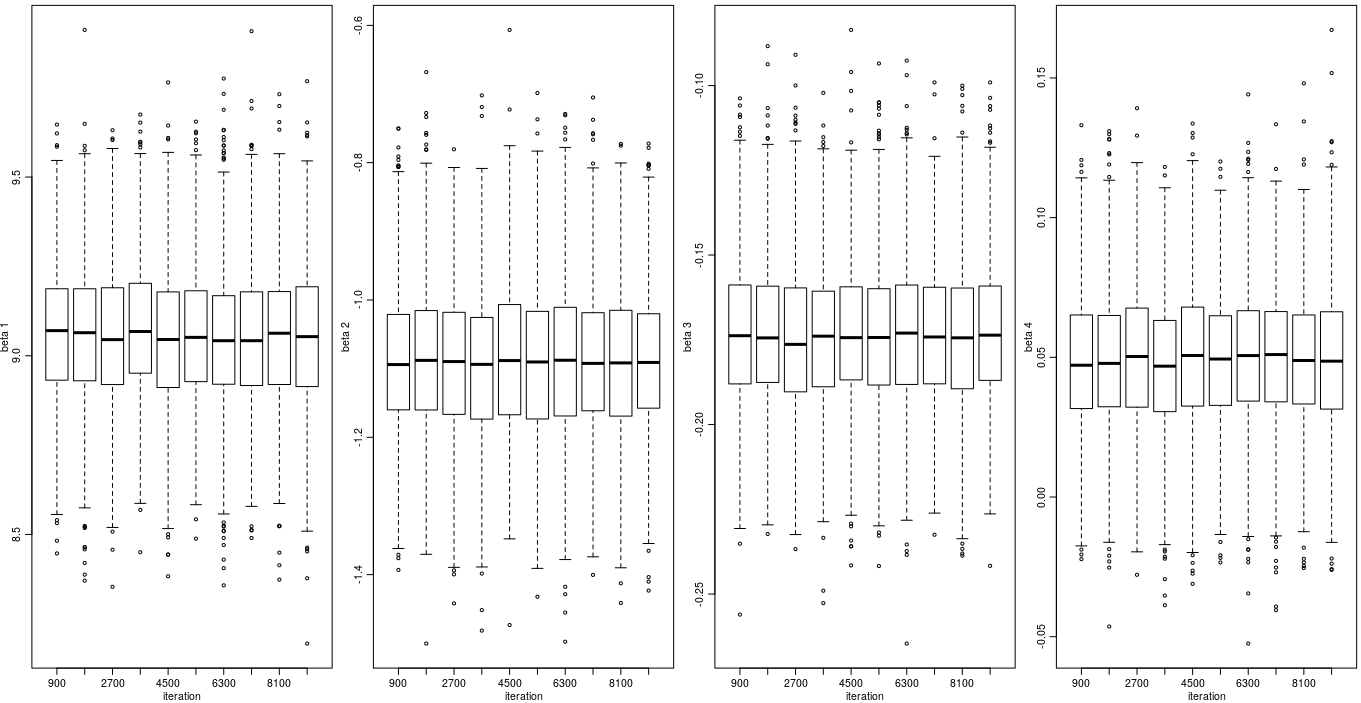
\includegraphics[width=160 mm]{pictures/negbin_single_r_stat.png}
	\caption{Stationarity analysis of the $\boldsymbol{\beta}$ regression parameters}
	\label{fig:nb_stat}
\end{figure}
\begin{figure}[H]
	\centering
	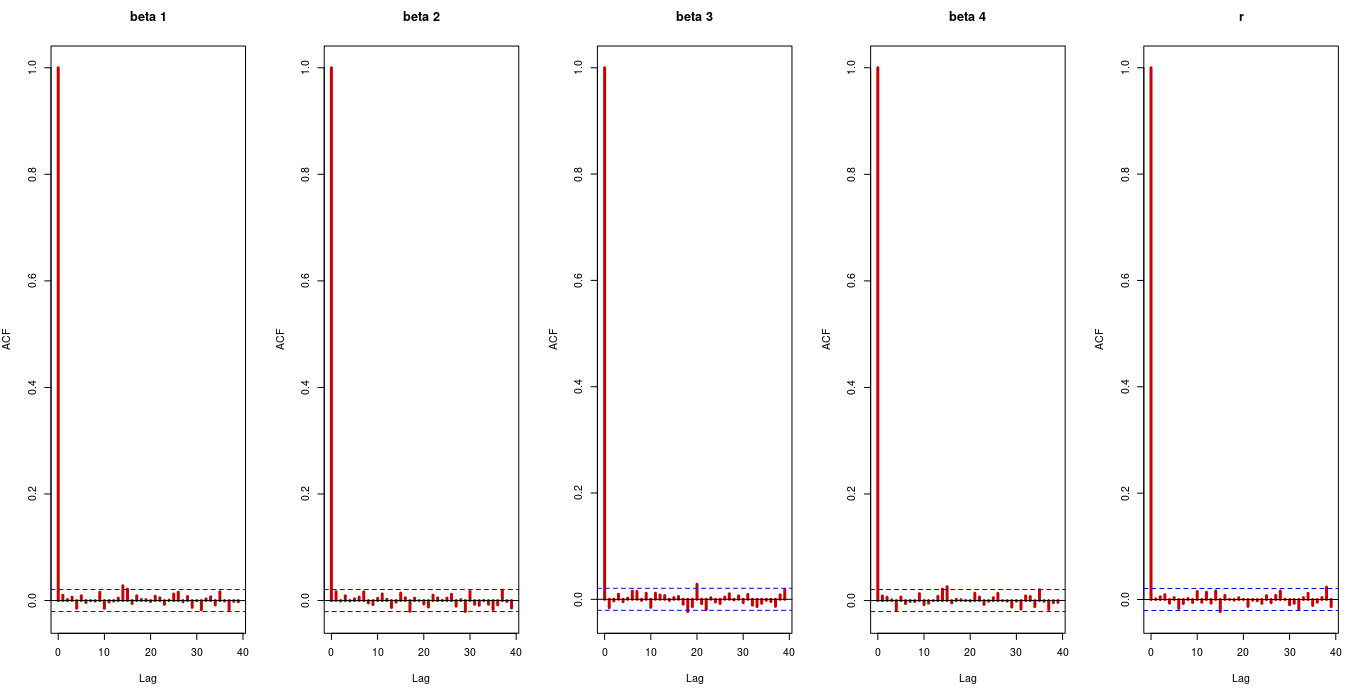
\includegraphics[width=160 mm]{pictures/negbin_single_r_acf.png}
	\caption{Autocorrelation plot of the $\boldsymbol{\beta}$ regression parameters and $r$ parameter}
	\label{fig:nb_acf}
\end{figure}
Regressors seem to be relevant, and their effects are coherent with the interpretation: during the weekend the total volume strongly decreases, rain has definitely a negative effect on the volume, while temperature positively impacts on $Y_t$.
Plots for regression parameters distributions follow:
\begin{figure}[H]
	\centering
	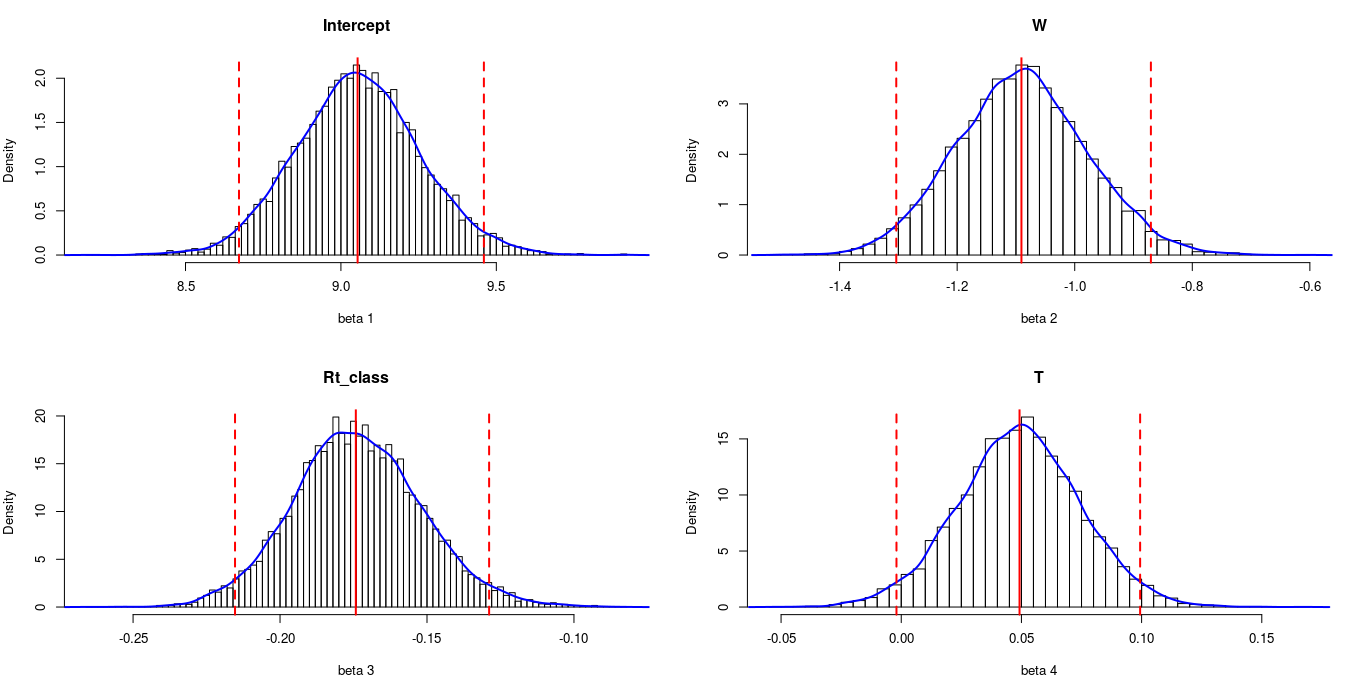
\includegraphics[width=160 mm]{pictures/negbin_single_r_beta.png}
	\caption{Distribution of the $\boldsymbol{\beta}$ regression parameters}
	\label{fig:nb_beta}
\end{figure}
Results of sampled $Y_t$ in correspondence to the 42 days under study are deeply different from the Poisson likelihood model. 90$\%$ credibility intervals are much larger, and the overall behaviour is caught. But the intervals widths are quite too large for real applications of the model, since the uncertainty described by the model determines too imprecise estimates. Here we show the situation:
\begin{figure}[H]
	\centering
	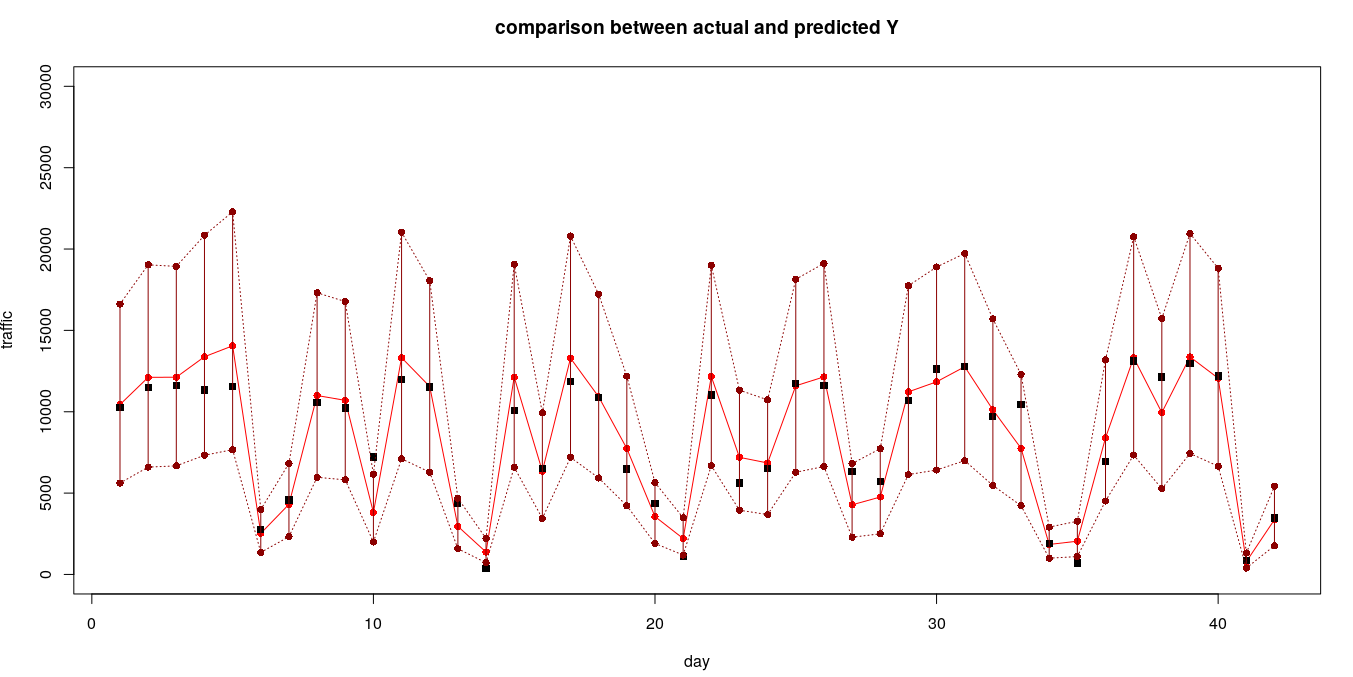
\includegraphics[width=160 mm]{pictures/negbin_single_r_pred.png}
	\caption{Sampled $Y_t$ for the 42 days, compared with the real data}
	\label{fig:nb_pred}
\end{figure}
We wondered if the highly different behaviour between weekends and weekdays could be better explained by introducing dispersion parameters $r$ specific for the two groups of days. On the other hand, we still assume the group effect on the mean of the distribution is only related to a global term: we suppose it does not affect rain and temperature influence on the response. The model proposed is a modification of the previous Negative Binomial likelihood:
\begin{model} Loglinear GLMM with Negative Binomial likelihood (2)\\
	\begin{equation*}
	\begin{aligned}
	&\textsc{Model}\\
	&Y_{tj}  |  p_{tj},r_j \overset{\independent}{\sim} NegBin(p_{tj},r_j), \ j = 1 (wkdays), 2 (wkends)\\
	&p_{tj} = \frac{r_j}{r_j+\mu_{tj}}\\
	&\log{\mu_{tj}} = \beta_1 + \beta_2R_{t} + \beta_3T_{t} + \theta_j\\
	&\\
	&\\
	\end{aligned}
	\qquad \qquad
	\begin{aligned}[c]
	&\textsc{Priors}\\
	&\beta_i | \tau_i \sim \mathcal{N}(0, \tau_i) \ i = 1,2,3\\
	&\tau_i \overset{\independent}{\sim} Gamma(2,10) \\
	&\theta_j | \tilde{\tau}_j \sim \mathcal{N}(0, \tilde{\tau}_j) \ j = 1,2\\
	&\tilde{\tau}_j \overset{\independent}{\sim} Gamma(2,10)\\
	&r_j \overset{\independent}{\sim}\mathcal{U}(0,50) \ j = 1,2
	\end{aligned}
\end{equation*}
	\end{model}
	We tried to implement the proposed model on Jags, but the chain was really badly simulated, as autocorrelation plots and stationarity were not acceptable, not even after long-time simulations. Therefore, we implemented the same model on Stan, which uses the alternative formulation with $\mu$ and $r$, and the diagnostic on the chain is definitely acceptable. Here we show the traceplots:
	\begin{figure}[H]
		\centering
		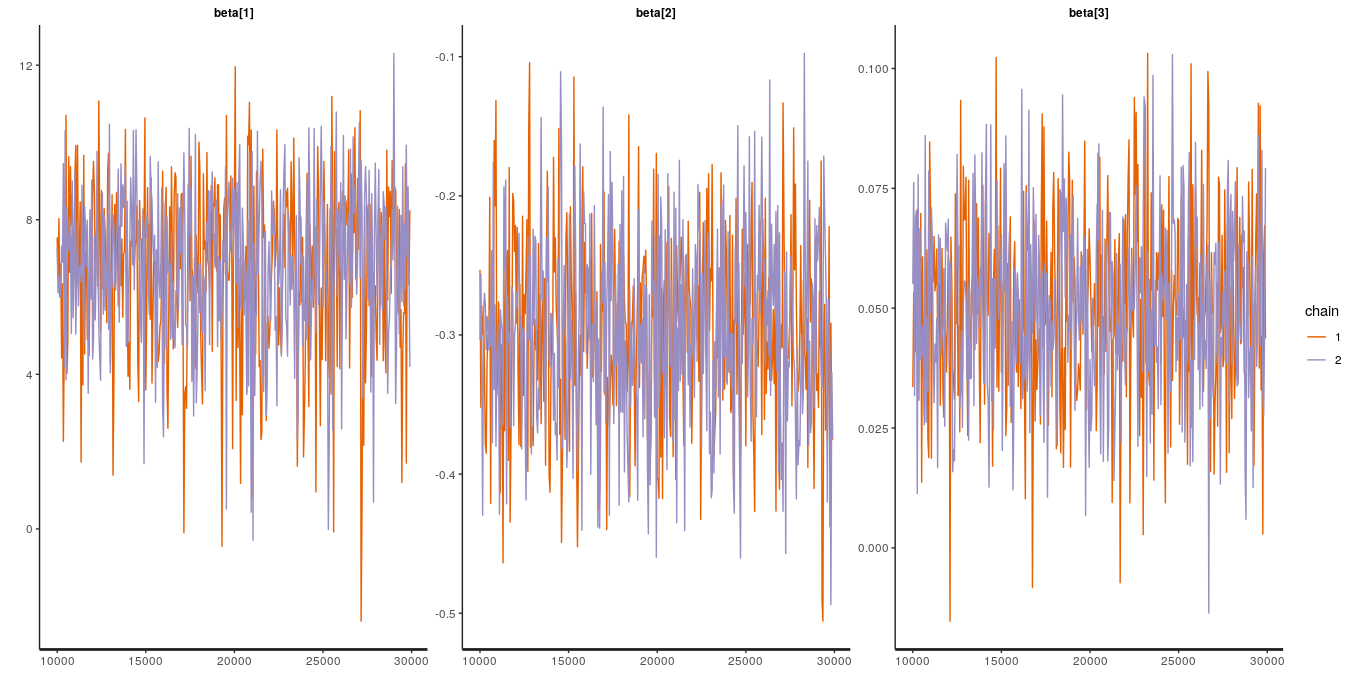
\includegraphics[width=110 mm]{pictures/negbin_double_r_trace_beta.png}
		\caption{Traceplots for $\boldsymbol{\beta}$ parameters}
		\label{fig:nb_d_trace_beta}
	\end{figure}
	\begin{figure}[H]
		\centering
		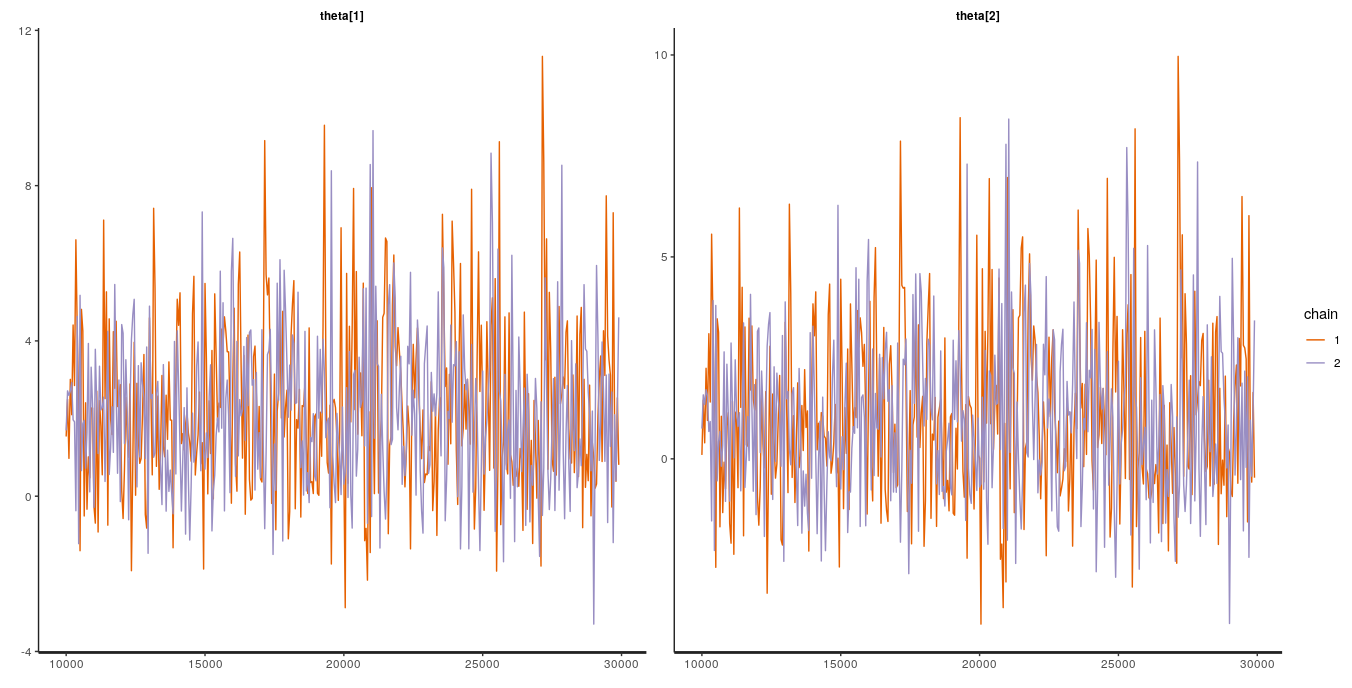
\includegraphics[width=130 mm]{pictures/negbin_double_r_trace_theta.png}
		\caption{Traceplots for $\boldsymbol{\theta}$ parameters}
		\label{fig:nb_d_trace_theta}
	\end{figure}
	We produced estimated distributions for fixed-effect $\boldsymbol{\beta}$ parameters and random-effect $\boldsymbol{\theta}$ parameters are:
	\begin{figure}[H]
		\centering
		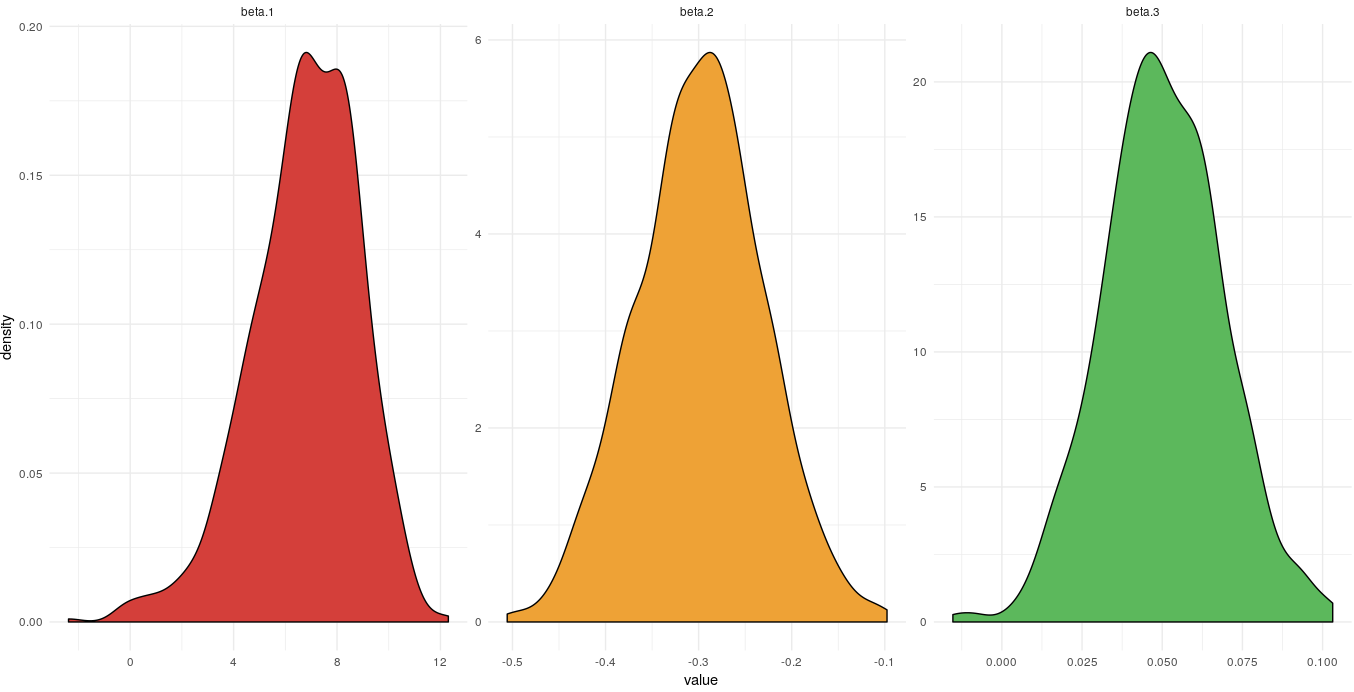
\includegraphics[width=130 mm]{pictures/negbin_double_r_beta.png}
		\caption{Posterior distribution of $\boldsymbol{\beta}$ parameters}
		\label{fig:nb_d_beta}
	\end{figure}
	\begin{figure}[H]
		\centering
		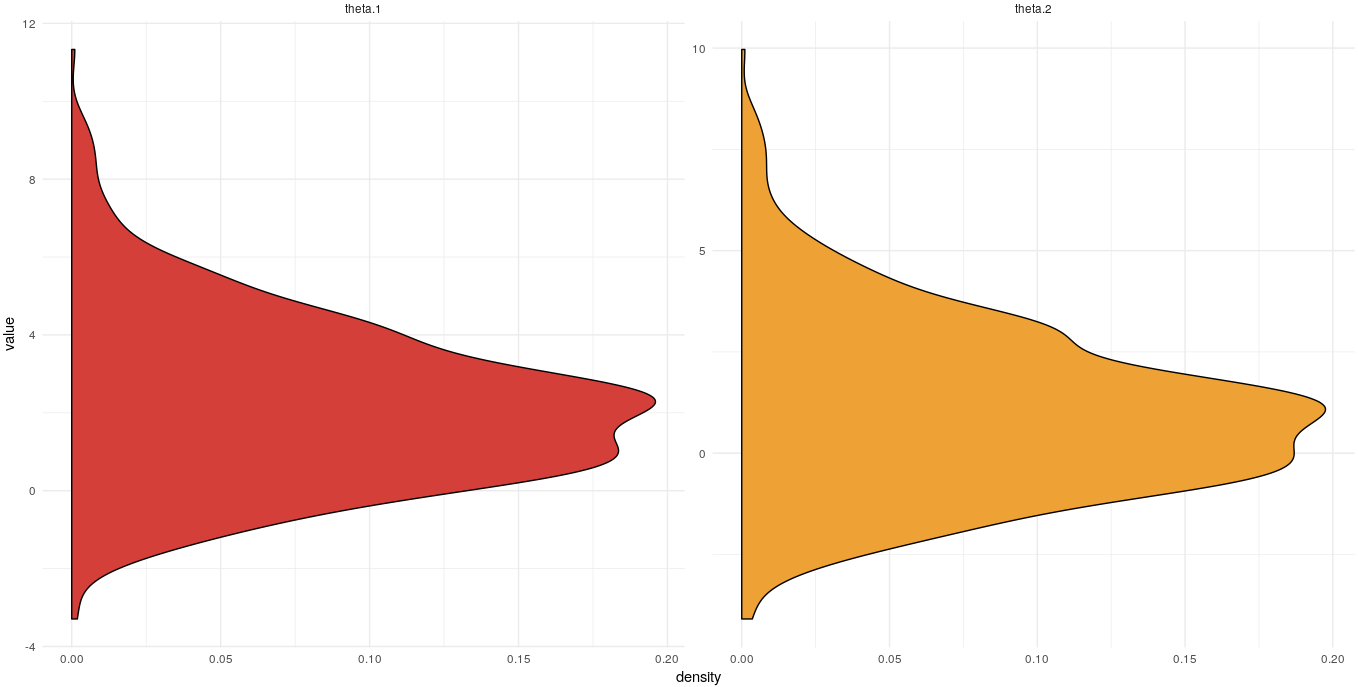
\includegraphics[width=132 mm]{pictures/negbin_double_r_theta.png}
		\caption{Posterior distribution of $\boldsymbol{\theta}$ parameters}
		\label{fig:nb_d_theta}
	\end{figure}
	The 90$\%$ credibility intervals of the corresponding 42 days prediction are shown in the following picture:
	\begin{figure}[H]
		\centering
		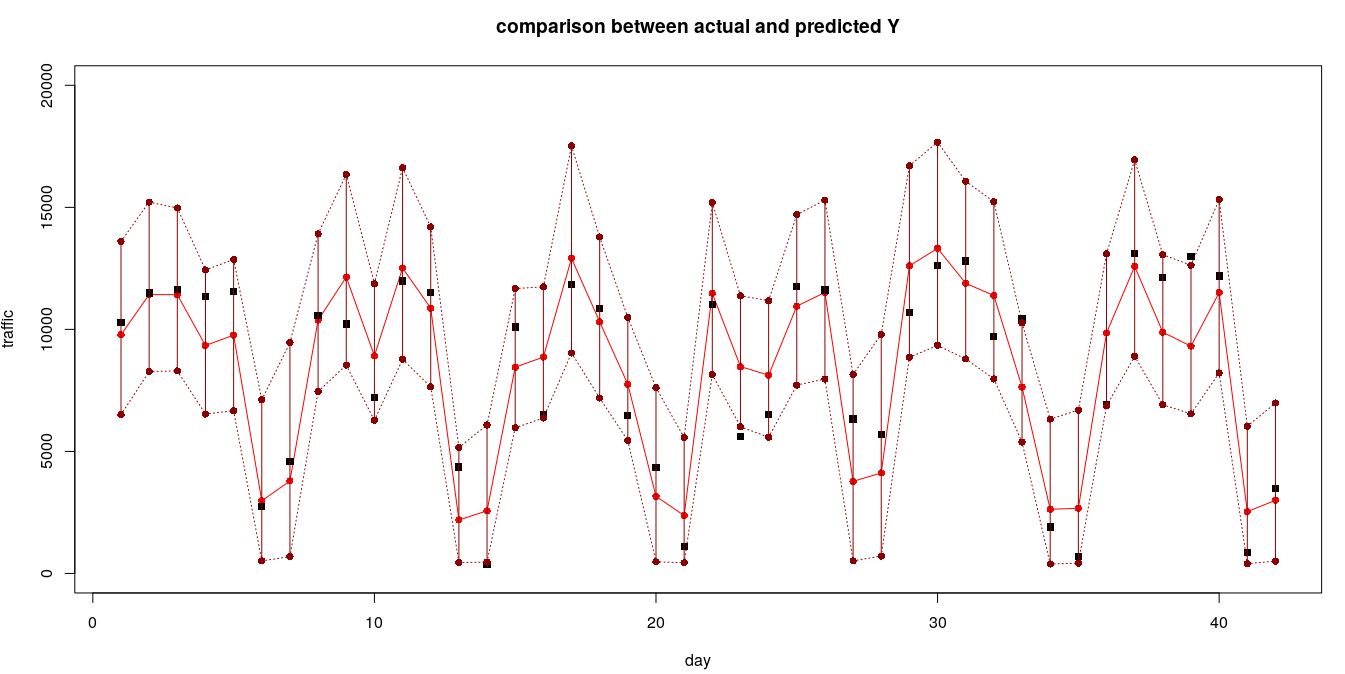
\includegraphics[width=160 mm]{pictures/negbin_double_r_pred.png}
		\caption{Sampled $Y_t$ for the 42 days, compared with the real data}
		\label{fig:nb_d_pred}
	\end{figure}
	This model seems to catch the overall phenomenon features, and the width of those intervals is shorter than the original Negative Binomial likelihood model. Only 4 data fall outside the associated intervals. However, the variance of our prediction is still quite high, so we wished to propose an even more suitable model for the problem.


\section{Bayesian Structural Time Series}
As a second operative approach, we tried to implement a Bayesian Structural Time Series model (BSTS). We can think this method as the Bayesian counterpart of the frequentis ARIMA representation: even though it does not rely on differencing, lags and moving averages, it makes possible to see historical data as the superposition of multiple effects, each one with its own meaning and interpretation. Moreover, the modularity of the BSTS approach, joint with the probability driven Bayesian model selection, makes it easier to quantify the posterior uncertainty of the individual components, perform variable
selection during model training, thus preventing overfitting, and also incorporate prior beliefs, possibly coming from time consistent, older data. 

\subsection{Introduction to BSTS}
Structural time series are basically state space models for historical data. In this subsection we will try to give a brief, but exhaustive, introduction to the topic stressing in particular the advantages deriving from the Bayesian approach, for a more complete and detailed description please refer to SV13 and JRN18 in bibliography.\\
\\
We can think a state space model as a couple of stochastic equations fed by independent noises and an initial condition:
\begin{equation}
\mathbf{y}_t = \mathbf{Z}_t \boldsymbol{\alpha}_t + \boldsymbol{\epsilon}_t,\quad \boldsymbol{\epsilon}_t \overset{\independent}{\sim} \mathcal{N}_m(0, \boldsymbol{\Sigma}_t),
\end{equation}
\begin{equation}
\boldsymbol{\alpha}_{t+1} = \mathbf{T}_t \boldsymbol{\alpha}_t + \mathbf{R}_t \boldsymbol{\eta}_t,\quad \boldsymbol{\eta}_t \overset{\independent}{\sim} \mathcal{N}_q(0, \mathbf{Q}_t),
\end{equation}
\begin{equation}
\boldsymbol{\alpha}_0 \sim \mathcal{N}_d(\boldsymbol{\mu}_0, \boldsymbol{\Sigma}_0)
\end{equation}
Borrowing the nomenclature from automatic control theory, the first relationship is called the observation equation, since it defines the $ \mathbb{R}^m$ vector of the observations at current time $ \mathbf{y}_t $ from the linear transformation $ \mathbf{Z}_t $ of a $ \mathbb{R}^d $ vector of the unobserved (and a priori fictitious) current latent states $ \boldsymbol{\alpha}_t $. The second identity is often known as transition equation, since it specifies latent states stochastic dynamics over time, or state equation. Within this context, $ d $ will be the overall number of latent states for all entries in $\mathbf{y}_t$ and model matrices $ \mathbf{Z}_t,\ \mathbf{T}_t,\ \mathbf{R}_t $ are made of known and unknown time varying parameters: $ \mathbf{Z}_t $ is the $ d \times m $ output matrix, $ \mathbf{T}_t $ is a $ d \times d $ transition matrix, and $ \mathbf{R}_t $ is a $ d \times q $ control matrix. $ \mathbb{R}^m $ vector $\boldsymbol{\epsilon}_t$ denotes observation errors with a $ m \times m $ variance matrix $ \boldsymbol{\Sigma}_t $, while $ \boldsymbol{\eta}_t $ is the $ q $-dimensional system error distributed with zero mean and a $ q \times q $ full rank state diffusion matrix $ \mathbf{Q}_t $, where $ q\leq d $. Finally the state is endowed with suitable random initial conditions.\\

There are two main advantages in the use of structural time series constructed in terms of components: first, each state variable can be analyzed both singularly or coupled together with the other effects, since addition of a new variable block is translated into a simple sum in terms of equations. This keeps the model representation elementary and enables evaluation through a Bayesian posterior probability approach. Moreover, provided state variables being added with criterion, state models can purposely give a meaningful interpretation for many building blocks of the scheme. As an example, just recall that in most ARIMA models the series is derived as the sum of a trend, the seasonality, maybe a local cycle and regression components, elicited through differentiation and use of moving averages. The state space counterpart of this, i.e. a quite flexible baseline for many STS models, can be written as:
\begin{equation}
\mathbf{y}_t = \boldsymbol{\mu}_t + \boldsymbol{\gamma}_t + \boldsymbol{\nu}_t + \boldsymbol{\beta}^T \mathbf{z}_t + \boldsymbol{\epsilon}_t
,\quad \boldsymbol{\epsilon}_t\overset{\independent}{\sim} \mathcal{N}_m(0, \boldsymbol{\Sigma}_t)
\end{equation}
where the summands are respectively trend, seasonality, cyclical component, regression and observation error. In the state space representation of before, $ \boldsymbol{\alpha}_t $ would be the vector containing these terms, $ \boldsymbol{\alpha}_t = [\boldsymbol{\mu}_t, \boldsymbol{\gamma}_t, \boldsymbol{\nu}_t, \mathbf{z}_t] $. However the model can undergo various simplifcations: often, for the sake of computation, $ \boldsymbol{\Sigma}_t=\boldsymbol{\Sigma}\ \forall t \in \{1:T\} $ is a constant positive definite matrix. Conversely, it can be also complicated as much as possible, for instance the regression summand might be made dynamic.

\subsection{Typical components of a state}
In this global setting the term of interest is the non-negative scalar $ y_t $ quantifying the overall amount of bikes crossing the city during a specific day. The data are available for $ i\in\{1:N=42\}$ and the goal of this section is finding an adequate state space and a suitable output equation able to capture the previous quantity in terms of some meaningful hidden latent variables. Let us discuss some candidate blocks that will be evaluated to derive the output.

\begin{itemize}
	\item The $ trend\ \mu_t$ will represent the baseline of the output. It is an a priori, unknown, slow varying function describing the total number of bikes running in a week, independently of the specific day. We can imagine this quantity as the state space counterpart of the moving average in SARIMA models: its dimension is the average volume of traffic in the period, therefore - whenever properly estimated - this term should not be affected by evident periodic variations. Conversely, its small and slow perturabations should somehow reflect protracted phenomena not direcly linked with the characteristics of a single day. For instance a long period of cold might affect people perception, discouraging the use of bikes even in a relatively temperate day. As a general rule, we might say that the trend is just the combined effect of everything that is neither due some local behaviour or the periodicity: in a purely ideal condition it should be just a perfect constant.\\
	\\ 
	The easiest way to add a trend to a state space model - just using linear equations - is that of defining a relationship of the form $ \mu_{t+1} = \mu_t +\eta_t $, with $ \eta_t\overset{iid}{\sim}\mathcal{N}(0,\frac{1}{\tau_\eta})\ \forall t\in\{1:n\}$. Please, pay attention to the fact that the notation is writen using precisions instead of variances. Within this framework, $ \{\mu_t\}_t $ is simply a random walk from the initial point. In order to make the estimate more robust, it is possible to add a second layer to the trend, thus allowing a locally linear behaviour: $\mu_{t+1} = \mu_t+\delta_t +\eta_t $ where $\delta_{t+1} = \delta_t +v_t $ (with $ v_t\overset{iid}{\sim}\mathcal{N}(0,\frac{1}{\tau_v})\ \forall t\in\{1:n\}$) represents the local slope of the process. Even if not explicitly written or requested, it is obvious that data fit well a model like this only if $ \tau_v $ and $ \tau_\eta $ estimates will be similar, possibly with greater precision on the slope. Using this argument recursively one might go even deeper in the depedencies chain, every time adding a linear term to the last one created, but this, in general, won't improve considerably the final result. Indeed, after a few iterations, the estimates will become more and more similar to irregular and small amplitude, highly uncertain noisy terms. For this reason, is quite common to stop immediately with the trend-slope approximation of the function.
	\item The $ periodicity\ \gamma_t $ will represent the core of a weekly based analysis like ours, since it defines a slow varying function whose shape repeats similarly - even though with slight variations during time - capturing, if summed to a proper trend, the simplest pure a priori estimate which could be proposed in absence of local informations concerning day-specific chracteristics (i.e. without local regressors), but simply averaging over a weakly based time window. Let $ S $ be the period, $ \gamma_t = \sum_{i=1}^{S-1}\gamma_{t+i-S} + w_t $ where $ w_t\overset{iid}{\sim}\mathcal{N}(0,\frac{1}{\tau_w})$ is the standard formula for this term. Note that even different periodicities coming from multiple periods can be added to the same trend, this way decomposing a maybe execedingly irregular periodic behaviour in simpler interpretable components. Usually, if two distinct blocks of this kind are added to a model, the one of greater period is usually referred to as $ periodic\ component $, while the other as $ inner\ cycle $.
	\item The $ autoregressive\ component\ \rho_t$ is a mesosclale term which is usually added to some models that have a strongly correleated behaviour not completely captured by local regression or periodicity and trend. It represents a sort of residual which may depend from its previous values during a fixed amount of past days, normally one or two. This parameter is definitely more problem specific than the previous ones and is rather uncommon, nevertheless, there are some cases in which it might prove useful.
	\item Finally most models sum a $regression $ block to the previous global terms, which adds a linear set of covariates to the aforementioned problem. The nature of this part might differ strongly from case to case: the regession may be static or dynamic in coefficients, it could use even mixed or mixture models in presence of actual or hypothesized multiple groups. In our case we will focus our attention to the variables of temperature and presence of rain which appeared to be the most relevant ones in the already concluded loglinear model.
\end{itemize}

\subsubsection{Regularized models}
Standard BSTS models use state at time $ t $ to predict the value that will be reached at $ t+1 $. Sometimes a little modification can be advisable, in particular in presence of abnormal irregularities on low variations functions, like trend or periodicity. Indeed, if a slow varying state appears to have a exceedingly oscillating behaviour - probably because the other terms have not been estimated with enough precision, due to the lack of data - a very effective strategy may lie in a forceful regularization. A typical smoothing applied in cases where there is a periodicity, is deriving the value at time $ t+1 $, not as function of the sole last value, but as its combined output with a vanishing weighted sum of the past analogue terms. As a final effect of this filtering, a more robust estimate for the quantiy of interest is produced, jointly to a dramatic decrease of the oscillations in slow varying functions. However, remember that this more robust method of estimation is better to be avoided in absence of oscillations, since it should lead in principle to similar results, but may even produce oversmoothing, in contrast with the initial purpose.

\subsection{Evaluation criteria}
Several similar models will be proposed and evaluated in this section, with the goal of establishing the best BSTS structure in capturing the generating process behind the data at our disposal. In order to reach that aim, we will stick to some simple but fundamental guidelines, summarized in the following catchphrases:

\begin{enumerate}
	\item performance is subject to correctness of modelling assumptions and proper diagnostics,
	\item use codified Beyesian tools to evaluate the worth of a model from a predictive viewpoint,
	\item in absence of strong evidence for a format let interpretability be the deciding factor,
	\item in case of a draw in the previous points, select the simplest paradigm.
\end{enumerate}

Let us now discus what will be the criteria that will guide the Bayesian evaluation:

\paragraph{Mean standardized residuals} As it can be easily inferred from previous subsections, the predictive distribution of vector $ \mathbf{y} $ is a joint gaussian, hence we can compare that density with the values attained in the data and compute the standardized residuals  of these values with respect to the laws. In an ideal model, these numbers should all be less than 2 and homoscedastically around the 0. In general, we might expect some outliers, and their number might be considered a rudimental tool of evaluation for both correctness and performance of a model. On the other hand, we can also take an average of the absolute value of the residuals and use this quantity as a tool to compare the predictive power of two models: the one reaching the smallest values shall be considered the best according to this criterion.
 
\paragraph{Mean tail probabilities} We can also compute the Bayesian p-values of our data, i.e. the probability of finding a number from the predictive distributions which is smaller/bigger than the ones got as datum (actually the minimum of these two quantities). These numbers should be as close to 0.5 as possible, meaning a centered datum w.r.t. the distribution. We can consider as evaluation methods both the quantity of outliers and the mean of these terms. The higher the mean, the better the model.

\paragraph{LOO-CV} The leave-one-out cross-validation is the most widely used tool in cases where the Watanabe-Akaike information criterion (WAIC) fails to be accurate (since it's a very close asymptotic approximation of the WAIC). The idea behind this method is quite clever, we will only tackle in brief its meaning, for further detail please refer to VGG16. The Bayesian LOO estimate of out-of-sample predictive fit is  
$elpd_{loo}= \sum_{i=1}^n \log(f(y_i|\mathbf{y}_{-i}))$ with $f(y_i|\mathbf{y}_{-i}) = \int_{\Theta}f(y_i|\boldsymbol{\theta})\pi(\boldsymbol{\theta}|\mathbf{y}_{-i})d\theta =CPO_i$
the leave-one-out predictive density given all data but the i-th observation, also known as conditional predictive ordinate. The LOO-CV method aims to maximize the $ elpd_{loo} $ in order to select the best model. There are many ways to approximate this quantity using MCMC samples, the traditional way is that of using chains to mimic an importance sampling, while the one implemented in the homonym command in $ \texttt{loo} $ R package is a more refined and advanced technique which uses Pareto smoothed importance sampling. Anyway, independently of the internal routines of the function, we can assume that this method, which may appear to be a bit overoptimistic with respect to the standard WAIC, but still very close to it in terms of results, should be preferred in cases of flat posteriors or uninformative priors and hence use it as our main evaluation tool in the following subsections.

\subsection{Proposed global models}
In this subsection we will provide a brief overview of the main global models considered in our work, stating and commenting where necessary each one of them, discussing the results in light of a Bayesian setting and finally comparing the different outputs. Let's start from the one that will represent the benchmark for any further variation.

\subsubsection{Standard with autoregression}
This model is a compendium of all the ingredients peculiar of standard BSTS structures discussed in the previous subsection. Within this framework, it is possible to represent the output as sum of a locally linear trend $ \mu $ (depending on $ \delta $), a period $ \gamma $, a 1-step $ \alpha $-autoregression $ \rho $ and a linear regression term $ \boldsymbol{\beta} $ on $ \mathbf{z}$ suitably selected covariates. The state is made of the aforementioned quantities and evolves fed by four independent noises (plus the noise in output equation). The scale of these five quantities is given in terms of their precisions, for which is set an hyperprior with a Gamma distribution and fixed hyperparameters. Also the initial conditions are formulated in coherent form, depending on fixed hyperparameters and being independent from the other terms. Finally an hyperprior can be fixed for the regression coefficients and the autoregression factor as independent normals. Just a remark concerning  notation: $ \tau $s are precisions, gaussians are written in terms of precisions instead of variances, and $ hpm $ stays for hyperparameters. In the appendix is possible to see an example of how to derive full conditionals for this kind of BSTS models and hence give direct implementation to a Gibbs sampler, without recurring to an already provided software.

\begin{model} Standard BSTS with autoregresion\\
\begin{equation*}
\begin{aligned}
&\textsc{Model}\\
&Y_t = \mu_t + \gamma_t + \rho_t + \boldsymbol{\beta}^T\mathbf{z}_t + \tau_\epsilon^{-\frac{1}{2}}\tilde{\epsilon}_t\\
&\mu_t = \mu_{t-1} + \delta_{t-1} +\tau_\eta^{-\frac{1}{2}}\tilde{\eta}_t\\
&\delta_t = \delta_{t-1} + \tau_v^{-\frac{1}{2}}\tilde{v}_t\\
&\gamma_t = \sum_{i=1}^{S-1}\gamma_{t+i-S} + \tau_w^{-\frac{1}{2}}\tilde{w}_t\\
&\rho_t = \alpha\rho_{t-1} + \tau_u^{-\frac{1}{2}}\tilde{u}_t\\
&\tilde{\epsilon}_t, \tilde{\eta}_t, \tilde{v}_t, \tilde{w}_t, \tilde{u}_t \overset{iid}{\sim} \mathcal{N}(0,1)\\
\\
&\textsc{Initial Conditions}\\
&\mu_0 \sim \mathcal{N}(m, \tau_m)\quad \quad \quad \quad \quad m, \tau_m\ hpm\\
&\delta_0 \sim \mathcal{N}(d, \tau_d)\quad \quad \quad \quad \quad \quad d, \tau_d\ \ hpm\\
&\boldsymbol{\gamma}_{0:(2-S)} \sim \mathcal{N}_{S-1}(\mathbf{g}, \tau_g\mathbf{I})\quad\ \ \mathbf{g}, \tau_g\ \ hpm\\
&\rho_0 \sim \mathcal{N}(r, \tau_r)\quad \quad \quad \quad \quad \quad \ r, \tau_r\ \ hpm\\
\\
\end{aligned}
\qquad \qquad
\begin{aligned}[c]
&\textsc{Priors}\\
&\boldsymbol{\beta} \sim \mathcal{N}_p(\mathbf{0}, \tau_b \mathbf{I})\ \ \quad \quad \quad \quad \quad \tau_b\ \quad \ hpm\\
&\alpha \sim \mathcal{N}(a, \tau_a) \ \quad \quad \quad \quad \quad \quad a, \tau_a\ \ hpm\\
&\tau_\epsilon \sim Gamma(a_\epsilon, b_\epsilon)\quad\ \quad \quad a_\epsilon, b_\epsilon\ \ hpm\\
&\tau_\eta \sim Gamma(a_\eta, b_\eta)\quad\quad \quad a_\eta, b_\eta\ \ hpm\\
&\tau_v \sim Gamma(a_v, b_v)\quad\quad \quad a_v, b_v\ \ hpm\\
&\tau_w\sim Gamma(a_w, b_w)\quad\quad\ a_w, b_w\ \ hpm\\
&\tau_u \sim Gamma(a_u, b_u)\quad\quad\quad a_u, b_u\ \ hpm\\
&\\
&\\
&\\
&\textsc{Independence}\\
&\{\tilde{\epsilon}_t, \tilde{\eta}_t, \tilde{u}_t, \tilde{w}_t, \tilde{v}_t, \mu_0, \delta_0, \boldsymbol{\gamma}_{0:(-S+2)}, \rho_0,\\ &\boldsymbol{\beta}, \alpha, \tau_\epsilon, \tau_\eta, \tau_v, \tau_w, \tau_u\}\\ &family\ of \independent real\ random\ variables\\
&\\
&\\
 \end{aligned}
\end{equation*}
\end{model}


Unfortunately, the dynamic behaviour of this model is unstable under uninformative prior selection. Hence, some simple variations had to be taken into account, together with the necessity of recurring to software in order to make computations with a Gibbs sampler: the decision lied upon JAGS. Two were the main issues destablizing the MCMC runs: having initial conditions with fixed precision (i.e. in general too precise w.r.t. the actual uncertainty of the subsequent time slots), and the uneven distribution of variability between state and output errors. In order to give homogeneity to the credibility of the initial conditions, we decided to set them, not as hyperparameters, but random, equal to the corresponding precisions of their dynamic equivalents. Moreover, it proved necessary to substitute the gamma distributions for the precisions with uniforms in intervals of suitable magnitude. The root of this decision is given by computational problems. If left free to evolve MCMC runs of JAGS tend to collect all the amount of uncertainty on the output error, leaving costant in time both trend and period. This detrimental and erratic coagulation of the uncertanty can be prevented forcing the state errors to keep a suitable - and reasonable - magnitude order (i.e. fixing a min/max for them). In general this produces better results and eventually the stability is preserved, since the posterior distributions of the precisions tend to be centered well inside adequately chosen intervals, somehow justifying $ a\ posterior $i the truncation. We now formalize the corrections.


\begin{model} Corrected standard BSTS with autoregrssion
	\begin{equation*}
	\begin{aligned}
	&\textsc{Model}\\
	&Y_t = \mu_t + \gamma_t + \rho_t + \boldsymbol{\beta}^T\mathbf{z}_t + \tau_\epsilon^{-\frac{1}{2}}\tilde{\epsilon}_t\\
	&\mu_t = \mu_{t-1} + \delta_{t-1} +\tau_\eta^{-\frac{1}{2}}\tilde{\eta}_t\\
	&\delta_t = \delta_{t-1} + \tau_v^{-\frac{1}{2}}\tilde{v}_t\\
	&\gamma_t = \sum_{i=1}^{S-1}\gamma_{t+i-S} + \tau_w^{-\frac{1}{2}}\tilde{w}_t\\
	&\rho_t = \alpha\rho_{t-1} + \tau_u^{-\frac{1}{2}}\tilde{u}_t\\
	&\tilde{\epsilon}_t, \tilde{\eta}_t, \tilde{v}_t, \tilde{w}_t, \tilde{u}_t \overset{iid}{\sim} \mathcal{N}(0,1)\\
	\\
	&\textsc{Initial Conditions}\\
	&\mu_0 \sim \mathcal{N}(m, \tau_\eta)\quad \quad \quad \quad \quad\  m\ \ hpm\\
	&\delta_0 \sim \mathcal{N}(d, \tau_v)\quad \quad \quad \quad \quad \quad d\ \ \ hpm\\
	&\boldsymbol{\gamma}_{0:(2-S)} \sim \mathcal{N}_{S-1}(\mathbf{g}, \tau_w\mathbf{I})\quad\ \ \mathbf{g}\ \ hpm\\
	&\rho_0 \sim \mathcal{N}(r, \tau_u)\quad \quad \quad \quad \quad \quad \ r\ \ hpm\\
	\\
\end{aligned}
\qquad \qquad
\begin{aligned}[c]
	&\textsc{Priors}\\
	&\boldsymbol{\beta} \sim \mathcal{N}_p(\mathbf{0}, \tau_b \mathbf{I})\ \ \quad \quad \quad \quad \quad \tau_b\ \quad \ hpm\\
	&\alpha \sim \mathcal{N}(a, \tau_a) \ \quad \quad \quad \quad \quad \quad a, \tau_a\ \ hpm\\
	&\tau_\epsilon \sim Unif(a_\epsilon, b_\epsilon)\quad\quad\ \quad \quad a_\epsilon, b_\epsilon\ \ hpm\\
	&\tau_\eta \sim Unif(a_\eta, b_\eta)\quad\quad\quad \quad a_\eta, b_\eta\ \ hpm\\
	&\tau_v \sim Unif(a_v, b_v)\quad\quad\quad \quad a_v, b_v\ \ hpm\\
	&\tau_w\sim Unif(a_w, b_w)\quad\quad\quad\ a_w, b_w\ \ hpm\\
	&\tau_u \sim Unif(a_u, b_u)\quad\quad\quad\quad a_u, b_u\ \ hpm\\
	&\\
	&\\
	&\\
	&\textsc{Independence}\\
	&\{\tilde{\epsilon}_t, \tilde{\eta}_t, \tilde{u}_t, \tilde{w}_t, \tilde{v}_t, \mu_0, \delta_0, \boldsymbol{\gamma}_{0:(-S+2)}, \rho_0,\\ &\boldsymbol{\beta}, \alpha, \tau_\epsilon, \tau_\eta, \tau_v, \tau_w, \tau_u\}\\ &family\ of \independent real\ random\ variables\\
	&\\
	&\\
\end{aligned}
\end{equation*}
\end{model}
\paragraph{Implementation}  The model has been implemented in bug language in order to be read by $ \texttt{rjags} $ package in R environment. Hyperparameters for precisions have been fixed in an uninformative way (using uniform distributions) or with extremely small precisions in case of gaussian density. All the values are detailed within this table:\\

\begin{table}[!htb]
	\begin{subtable}{.5\linewidth}
		\centering
\begin{tabular}{|c|c|c|c|c|c|}
	\hline
	& $ \tau_\epsilon $ & $ \tau_\eta $ &$  \tau_v $ & $ \tau_w $ & $ \tau_ u $\\
	\hline
	a &$  1\mathrm{e}{-7} $ & $  1\mathrm{e}{-5} $ &$  1\mathrm{e}{-5} $&$  1\mathrm{e}{-5} $&$  1\mathrm{e}{-5} $\\
	\hline
	b &$  1\mathrm{e}{-4} $ & $  1\mathrm{e}{-4} $ &$  1\mathrm{e}{-4} $&$  1\mathrm{e}{-4} $&$  1\mathrm{e}{-3} $\\
	\hline
\end{tabular} 
	\end{subtable}%
	\begin{subtable}{.5\linewidth}
		\centering
	\begin{tabular}{|c|c|c|c|c|}
		\hline
		& $ \tau_\alpha $ & $ \tau_\beta $ & $ r $ & $ d $\\
		\hline
		value &$  1\mathrm{e}{-5} $ & $  1\mathrm{e}{-5} $& 0 & 0\\
		\hline
	\end{tabular} 
	\end{subtable} 
\end{table}

For what concerns $ m $ and $ \mathbf{g} $, their value is assigned using the estimate provided by moving average and periodicity from the frequentist statistical tools discussed in the preliminary phase. This choice is made in order to set the initial conditions at a reasonable value, taking advantage of the conceptual link between STS periodicity and filtered priodicity, trend and moving average, as pointed out in the previous section. The regression $ \boldsymbol{\beta}^T\mathbf{z} $ part can be expressed as $ (\beta_1+\nu_1w)z_1 + (\beta_2+\nu_2w)z_2$, a mixed effect model of the kind $ \mathit{common\ value + group\ specific\ correction} $. $ w $ is an indicator function that takes either value $ 1 $, if the day is part of a weekend, or $ 0 $ else; $ z_1 $ and $ z_2 $ are respectively a scaled factor denoting the amount of rain forecasted for the day and the average daily temperature registered. These covariates are among the ones suggested by both the frequentists analyisis and the loglinear model selection. We will discuss their importance and role in the following paragraphs.

\paragraph{Diagnostics}
Let us discuss the godness of the chains produced by JAGS MCMC samples.
The following boxplots enlight about both the stability and the values assumed by the parameters. As we can see, after having run approximately 500000 samples with a thinning of 20 units in order to avoid high autocorrelation and 10000 units burnin, we have reached a good degree of stationarity.

\begin{figure}[H]
	\begin{subfigure}[H]{0.50\linewidth}
	\centering
	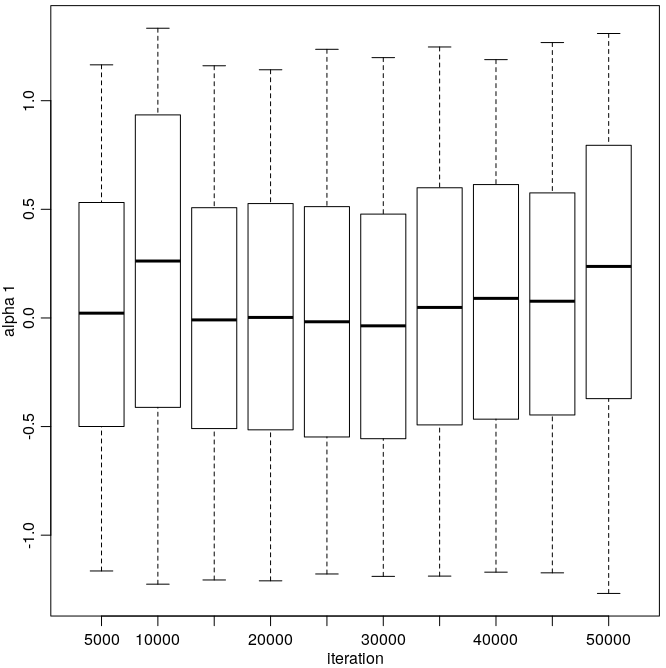
\includegraphics[width=70 mm]{pictures/m2_s1.png}
	\caption{Boxplot of $ \alpha $ samples}
	\label{fig:M2_s1}
\end{subfigure}
\hfill
\begin{subfigure}[H]{0.50\linewidth}
	\centering
	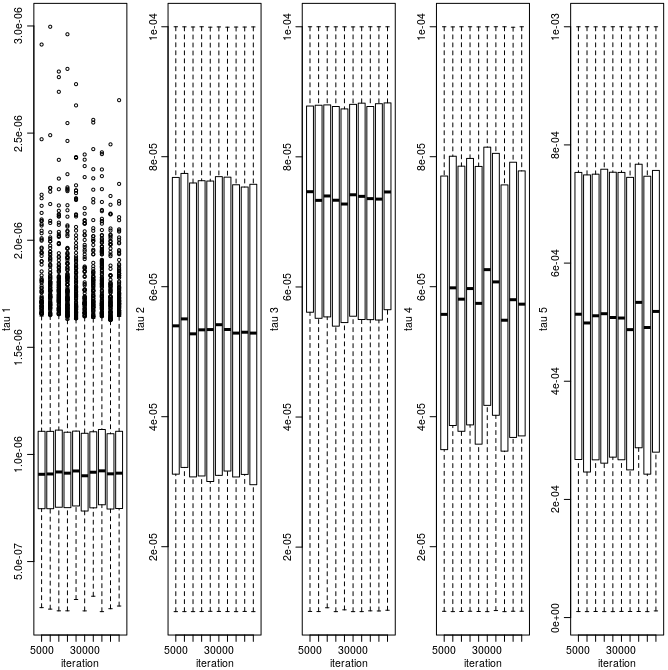
\includegraphics[width=70 mm]{pictures/m2_s2.png}
	\caption{Boxplot of $ \tau $ samples}
	\label{fig:M2_s2}
\end{subfigure}%
\vfill
	\begin{subfigure}[H]{0.50\linewidth}
	\centering
	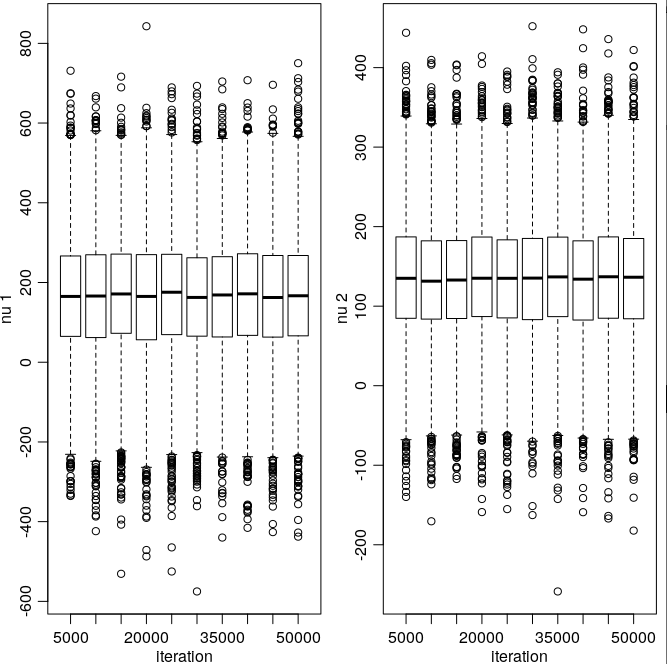
\includegraphics[width=70 mm]{pictures/m2_s3.png}
	\caption{Boxplot of $ \nu $ samples}
	\label{fig:M2_s3}
\end{subfigure}
\hfill
\begin{subfigure}[H]{0.50\linewidth}
	\centering
	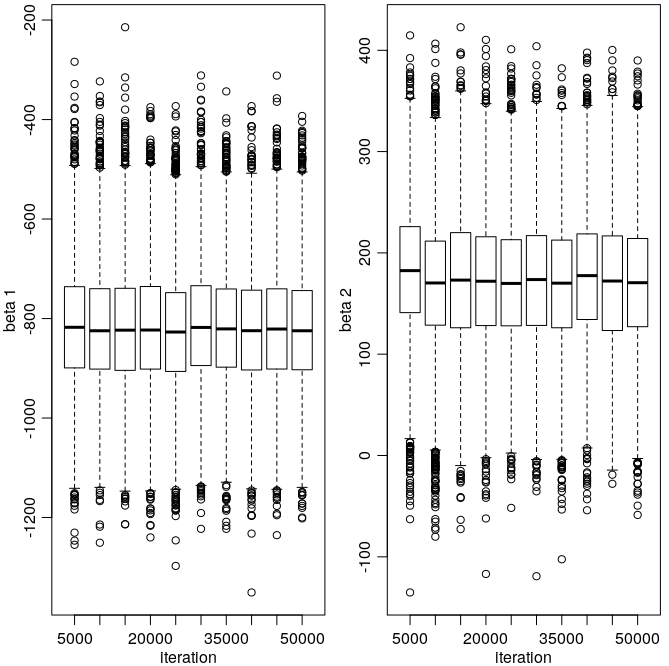
\includegraphics[width=70 mm]{pictures/m2_s4.png}
	\caption{Boxplot of $ \beta $ samples}
	\label{fig:M2_s4}
\end{subfigure}%
	\caption{Model boxplots}
\end{figure}

From the figures it appears quite clear that factor $ \alpha $ is not likely to be cosidered different form zero, since its distribution appears completely centered on that value, thus making the autoregressive part seem definitely useless. Different argument for terms $ \beta $ and their $ \nu $ corrections: on the opposite they have values quite strongly differing from 0. Note in particular that the first coefficient $ \beta_1 $, linked to the presence of rain, is negative, just as it was expcted. On the other hand, the second coefficent, more direcly linked with temperature is positive, thus entailing that a mild climate should have a positive impact on the number of trips. Recall also that $ \nu $ terms represent the correction in presence of weekends. Apparently, rain has a weaker effect in these days (probabily due to the overall decreasing amount of traffic), where instead high temperature seems to ease runs even more than during weekdays. Nonetheless, it should appear clear that $ \nu $ values are highly variable and so not completely credible. A larger dataset may probably be needed in order to get a better grasp of the real nature of these values and thus ascertain with a greater degree of confidence their actual worth in the model.\\
\\
Let's now discuss the chain mixing of the Gibbs sampler's MCMC runs used by JAGS to draw posterior distributions. First some technical details: we have run two chains of 500000 iterations each, with a burnin of 10000 and a thinning each 20 or 100. Results are quite similar in both cases, even when the thinning is selected at the smaller quantity. However if we want to see nice autocorrelation plots we need to reach at least the second value. As it can easily be deduced from the following pictures, autocorrelation plots are acceptable in all cases but on term $ \beta_2 $ which appears very autocorreleated, even though the final shape of the distribution seems to match pretty well that of a gaussian. Opposite behaviour for $ \alpha $ which has a completely uniform nature, testifying the lack of precision in this term estimation (luckily, note that this factor is so small to not influence very much the rest). Nonetheless, given the poor performances and weak worth, we will discuss the elimination of this factor in further developments. We now report the autocorrelation plots, distributions and traceplots of the most relevant parameters in our model.

\begin{figure}[H]
	\begin{subfigure}[H]{0.50\linewidth}
		\centering
		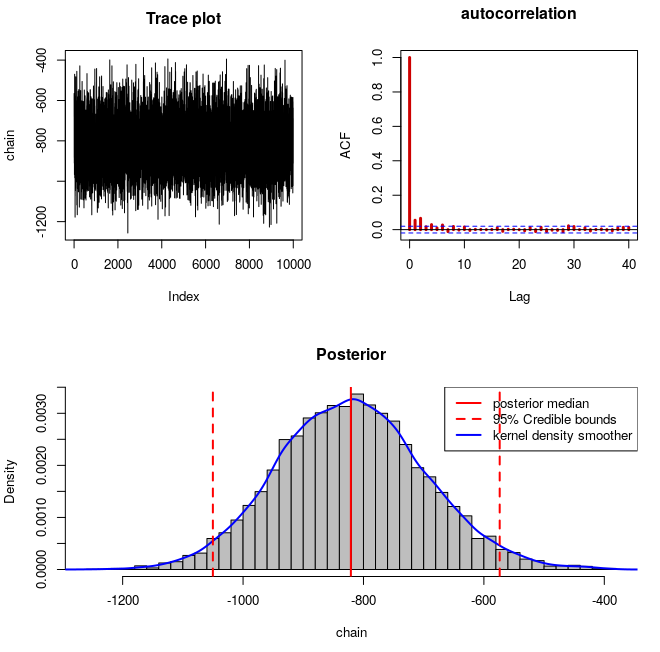
\includegraphics[width=65 mm]{pictures/beta_1.png}
		\caption{Diagnostics for $ \beta_1 $ samples}
		\label{fig:beta_1}
	\end{subfigure}
	\hfill
	\begin{subfigure}[H]{0.50\linewidth}
		\centering
		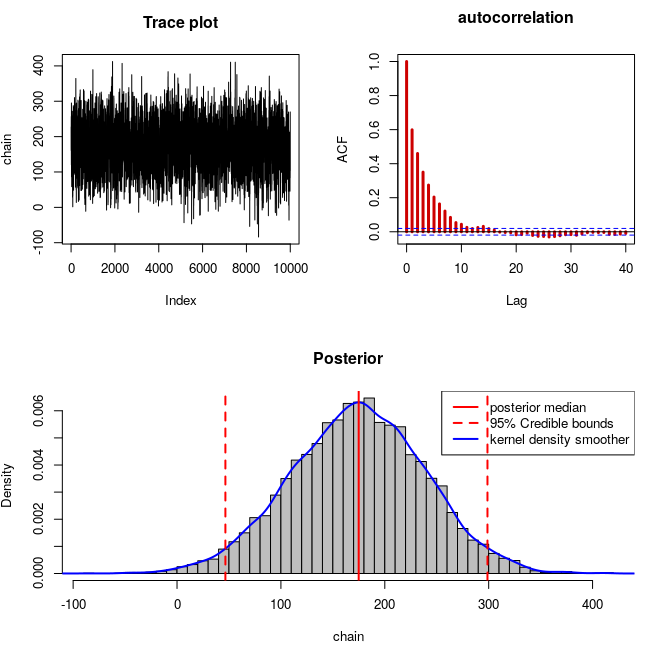
\includegraphics[width=65 mm]{pictures/beta_2.png}
		\caption{Diagnostics for $ \beta_2 $ samples}
		\label{fig:beta_2}
	\end{subfigure}%
	\vfill
	\begin{subfigure}[H]{0.50\linewidth}
		\centering
		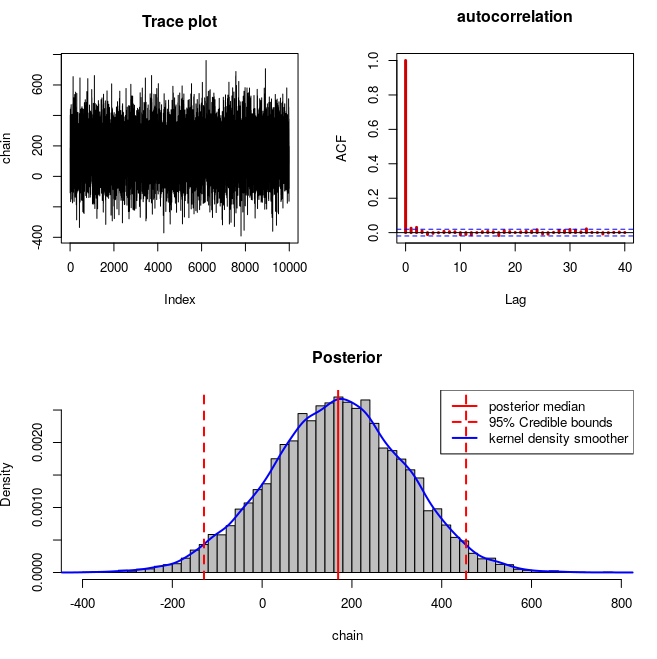
\includegraphics[width=65 mm]{pictures/nu_1.png}
		\caption{Diagnostics for $ \nu_1 $ samples}
		\label{fig:nu_1}
	\end{subfigure}
	\hfill
	\begin{subfigure}[H]{0.50\linewidth}
		\centering
		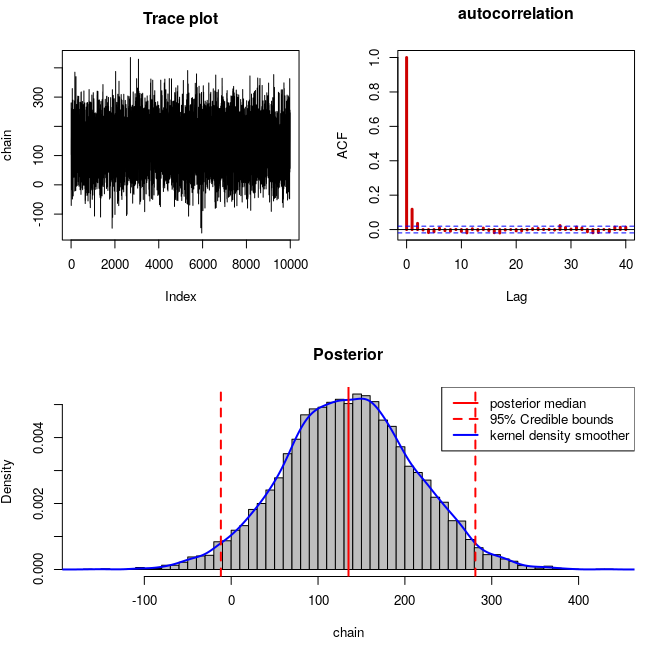
\includegraphics[width=65 mm]{pictures/nu_2.png}
		\caption{Diagnostics for $ \nu_2 $ samples}
		\label{fig:nu_2}
	\end{subfigure}%
\end{figure}

\begin{figure}[H]
		\centering
		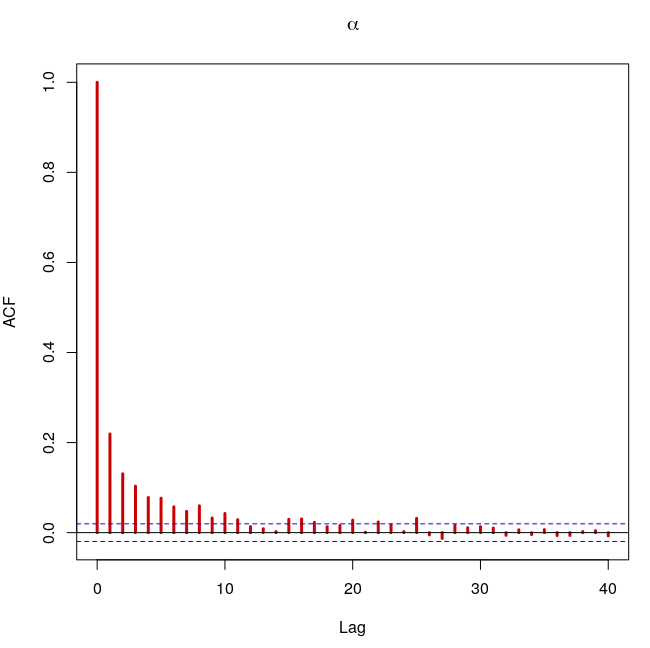
\includegraphics[width=60 mm]{pictures/alpha.png}
		\caption{Autocorrelation for $ \alpha $ samples}
		\label{fig:alpha}
\end{figure}

We don't report the traceplots of all $ \mu $s and $ \gamma $s etc.., otherwise we would need tons of ink, however rest assured that their shape is precisely matching that of a gaussian and traceplots are fat enough also in these terms. We can get an idea of the simmetry specially looking at some results in the next paragraph.

\begin{figure}[H]
		\centering
		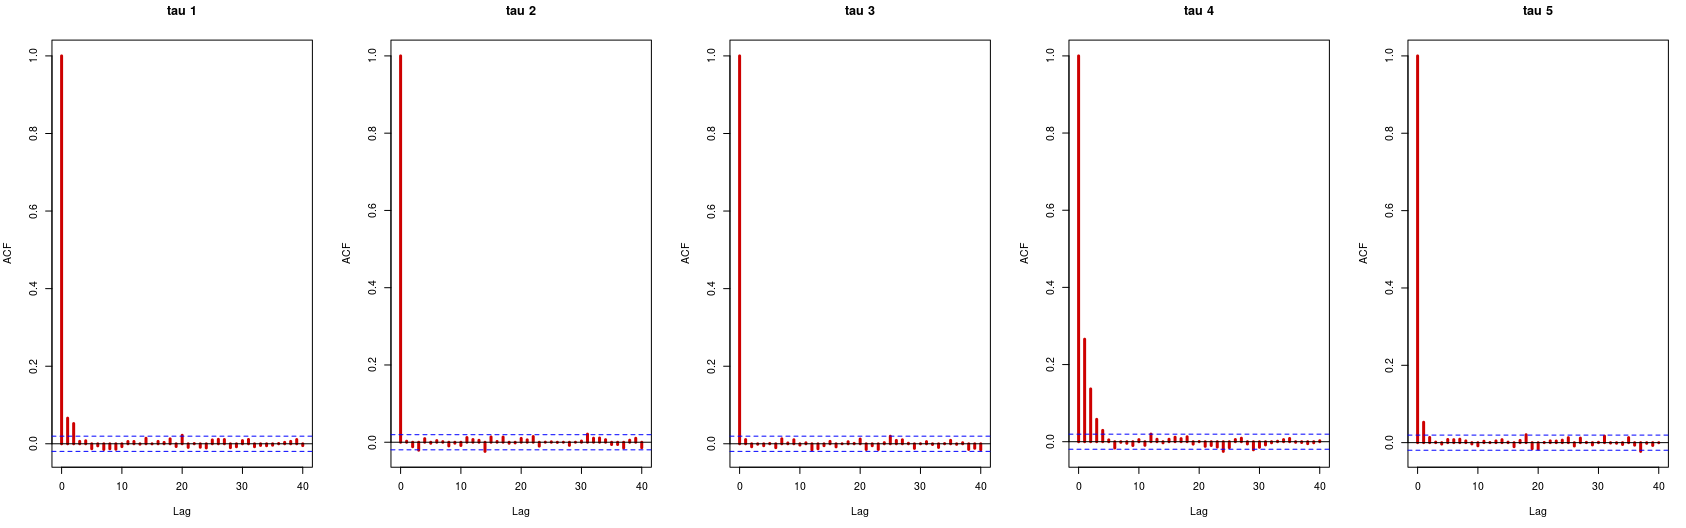
\includegraphics[width=160 mm]{pictures/tau.png}
		\caption{Autocorrelation for $ \tau $ samples}
		\label{fig:tau}
\end{figure}

\paragraph{Results}
We  will now discuss in detail the results produced by this model, provided its validation from a diagnostic viewpoint. In particular we will focus on the structural capability of predicting the outcome of the time series, i.e. how close does our prediction come with respect to the actual observed data.

\begin{figure}[H]
		\centering
		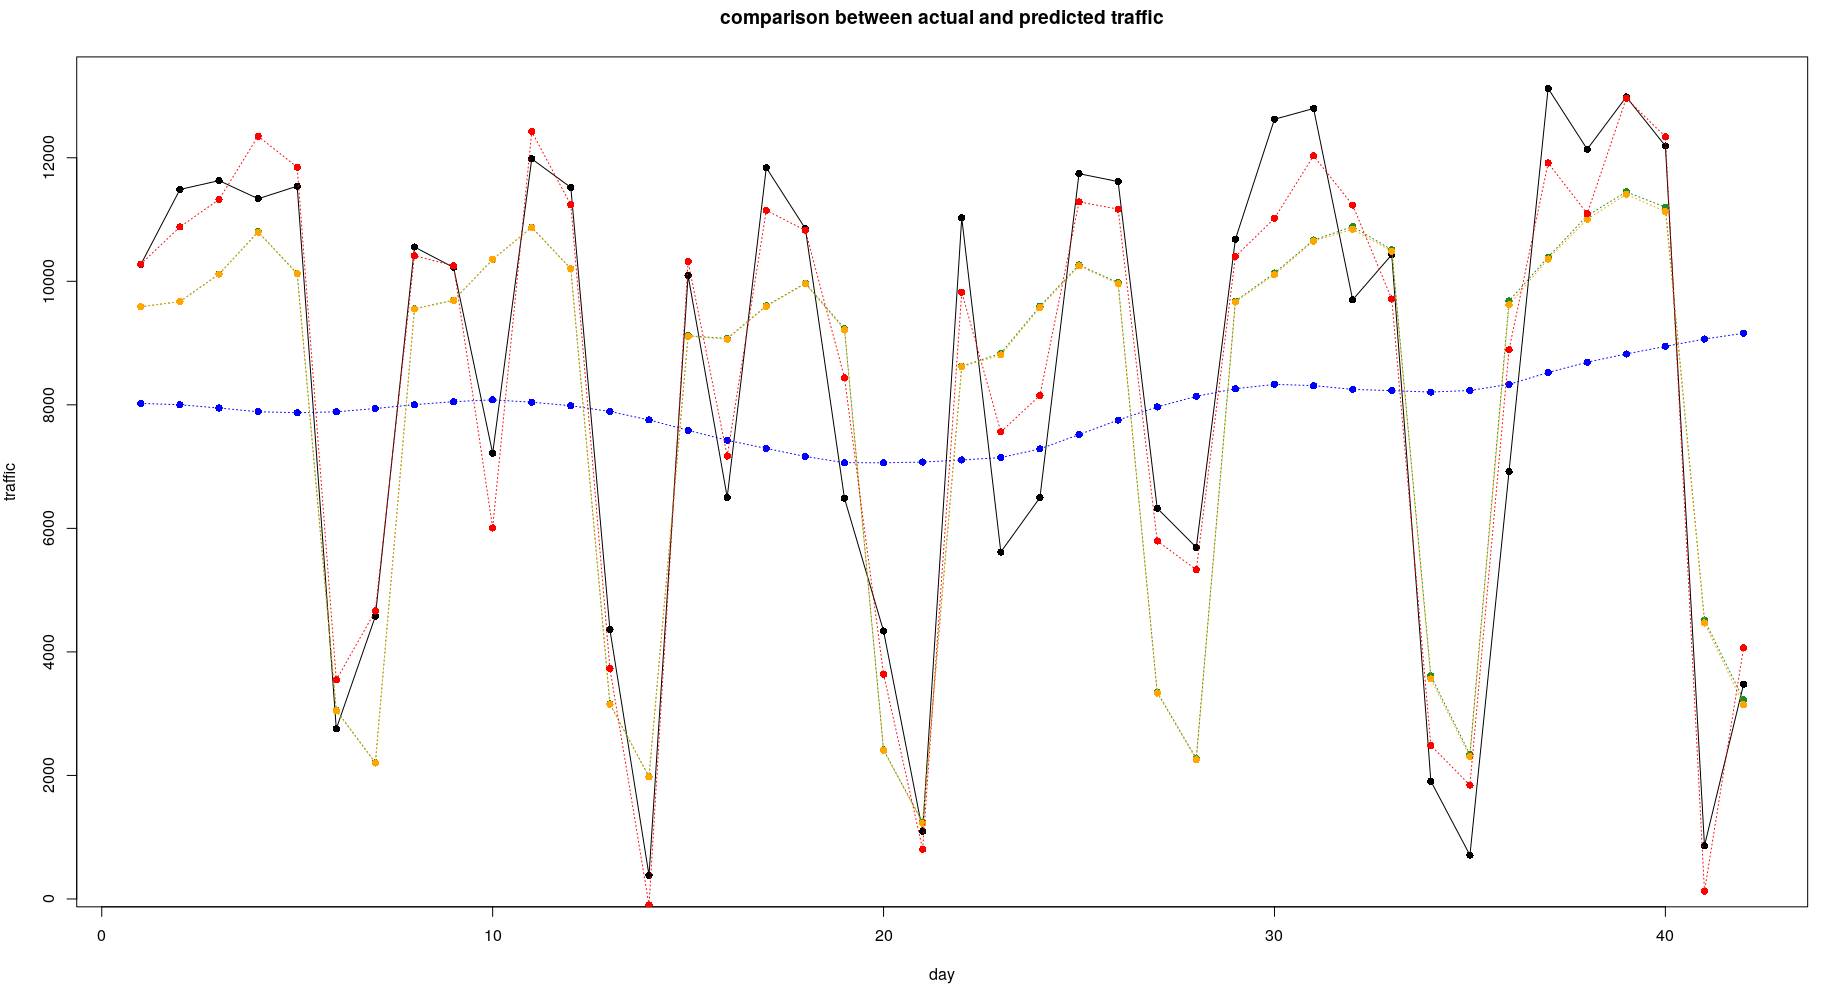
\includegraphics[width=150 mm]{pictures/m2_g1.png}
		\caption{Sum of trend (blue), periodicity (green), autoregression (yellow) and regression (red)}
		\label{fig:M2_p1}
	\end{figure}

In picture \ref{fig:M2_p1} it is possible to see the superposition of different components of the state and the prediction that can be deduced from them. It is evident that both trend and periodicity are perfectly in line with their abstract meaning and note that this fact is absolutely not trivial since the evolution of the MCMC is completely free and driven only by the rules constituting the model. In principle the final solution might had stabilized to values very far from the intuitve meaning that we gave to these terms of the state. Seeing our intuition being met is surely an indirect hint showing the model's ability to capture the essence of the process generating the data. Moreover the fact that the functions are slow varying may suggest us the avoidability of a robust method, that we will however try anyway for the sake of comparison. Coversely, just as pointed out during the diagnostics phase the action of the autoregression part seems irrelevant since the yellow and green line are almost cohincident. 
\begin{figure}[H]
		\centering
		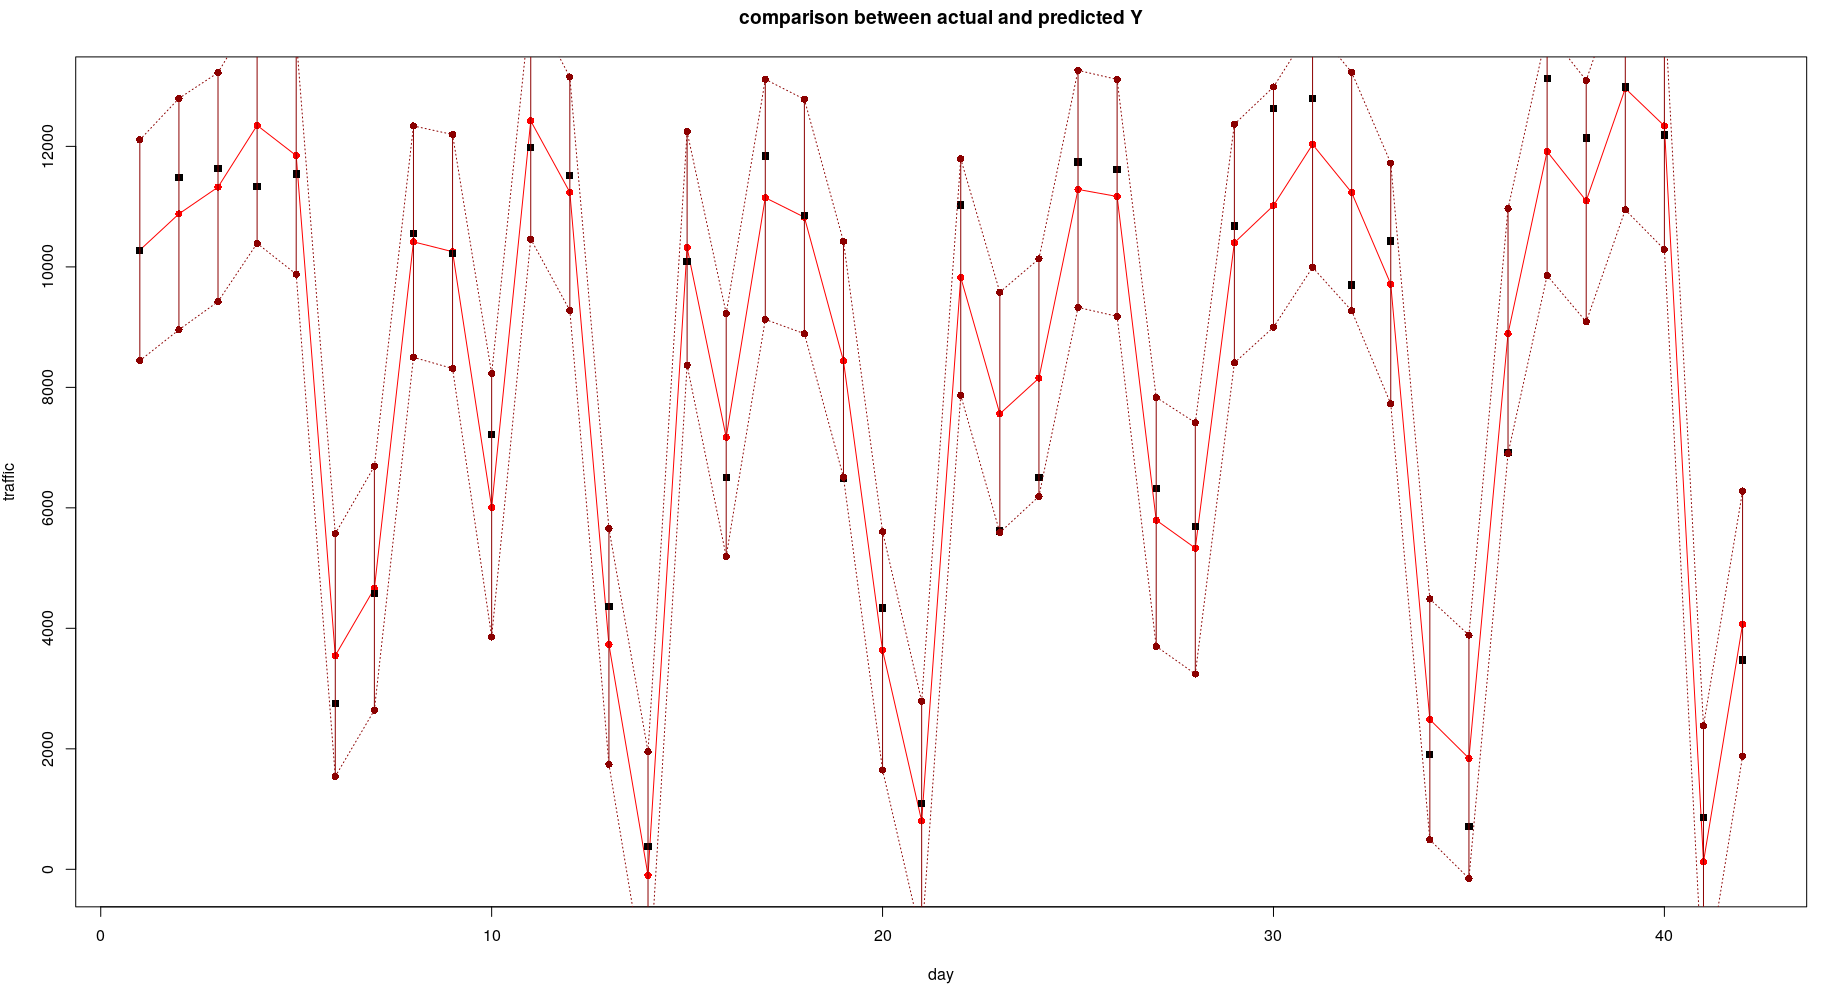
\includegraphics[width=150 mm]{pictures/m2_g2.png}
		\caption{90\% credibility intervals in dark red, in black the true responses $ y $}
		\label{fig:M2_p2}
\end{figure}
Fundamental is also the role of the regression component that, summed to aforementioned parts is able to capture quite well the shape of the original function. In particular the slope of some increments changes between pre and post addition of the regression to the model and mostly of the times this change meets what actully happens in the original profile. This can be considered a positive signal, since trend, periodicity and autoregression are good only to fix the mesocale form of the function, the local behaviour is very difficult to be captured by these terms. The fact that a strong positive correction is performed by the addition of the linear regression entails the presence of a strong local dependence. This fact is absolutely coherent with what is supposed to happen in reality since, very often, it is up to the climatic conditions to dictate the effective number of bikes moving on the network on a certain day. The second picture \ref{fig:M2_p2} shows the 90\% credibility intervals of the predicted $ y $s. As it can be seen the amplitude of these lines is around the 2000 units, since the standard deviation of our dstribution is approximately of 1000 trips. Moreover, almost all the times, data lie within the intervals suggested by the model.

\begin{figure}[H]
	\begin{subfigure}[H]{0.5\linewidth}
		\centering
		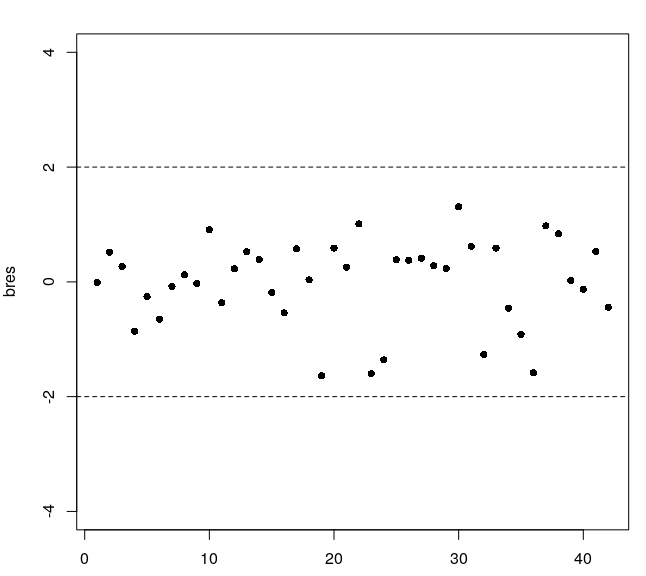
\includegraphics[width=70 mm]{pictures/m2_bres.png}
		\caption{Normalized residuals behaviour}
		\label{fig:M2_res}
	\end{subfigure}
	\hfill
	\begin{subfigure}[H]{0.5\linewidth}
		\centering
		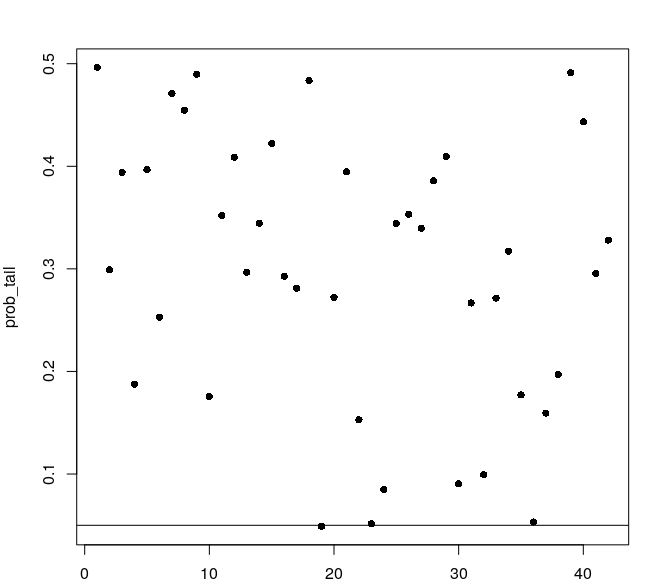
\includegraphics[width=70 mm]{pictures/m2_out.png}
		\caption{Outlier observations identification}
		\label{fig:M2_out}
	\end{subfigure}%
	\caption{Results produced by the model}
\end{figure}

As pointed out by the figure, there is just a small portion (2-3 among 42) of data which are not captured well by the model and often belong to days with a strong - but short - rainy phenomena, for which the scale factor is too vague in order to take into account sharp variations in the same day and only one possibility can be accepted (the day have to be classified either as sunny or rainy according to the information at our disposal, hence making impossibe a more detailed level of prediction). For this reason, as a final comment, we can consider the model designed in this paragraph a good staring point from which to try some improvements or simplifications. We will mainly focus on three variants: without temperature as a covariate, without autoregression and the robust version. Finally let us conclude this pragraph with the plot of a possible prediction of the future done by the chain, using the predictor which minimizes quadratic loss (expected value) and reporting 90\% confidence bands. A short remark, given the strong stability of the prediction we might expect not to be necessary a robut version of it. We will clarify this point in a didicated section where comparisons will be made from a predictive viewpoint.

\begin{figure}[H]
	\centering
	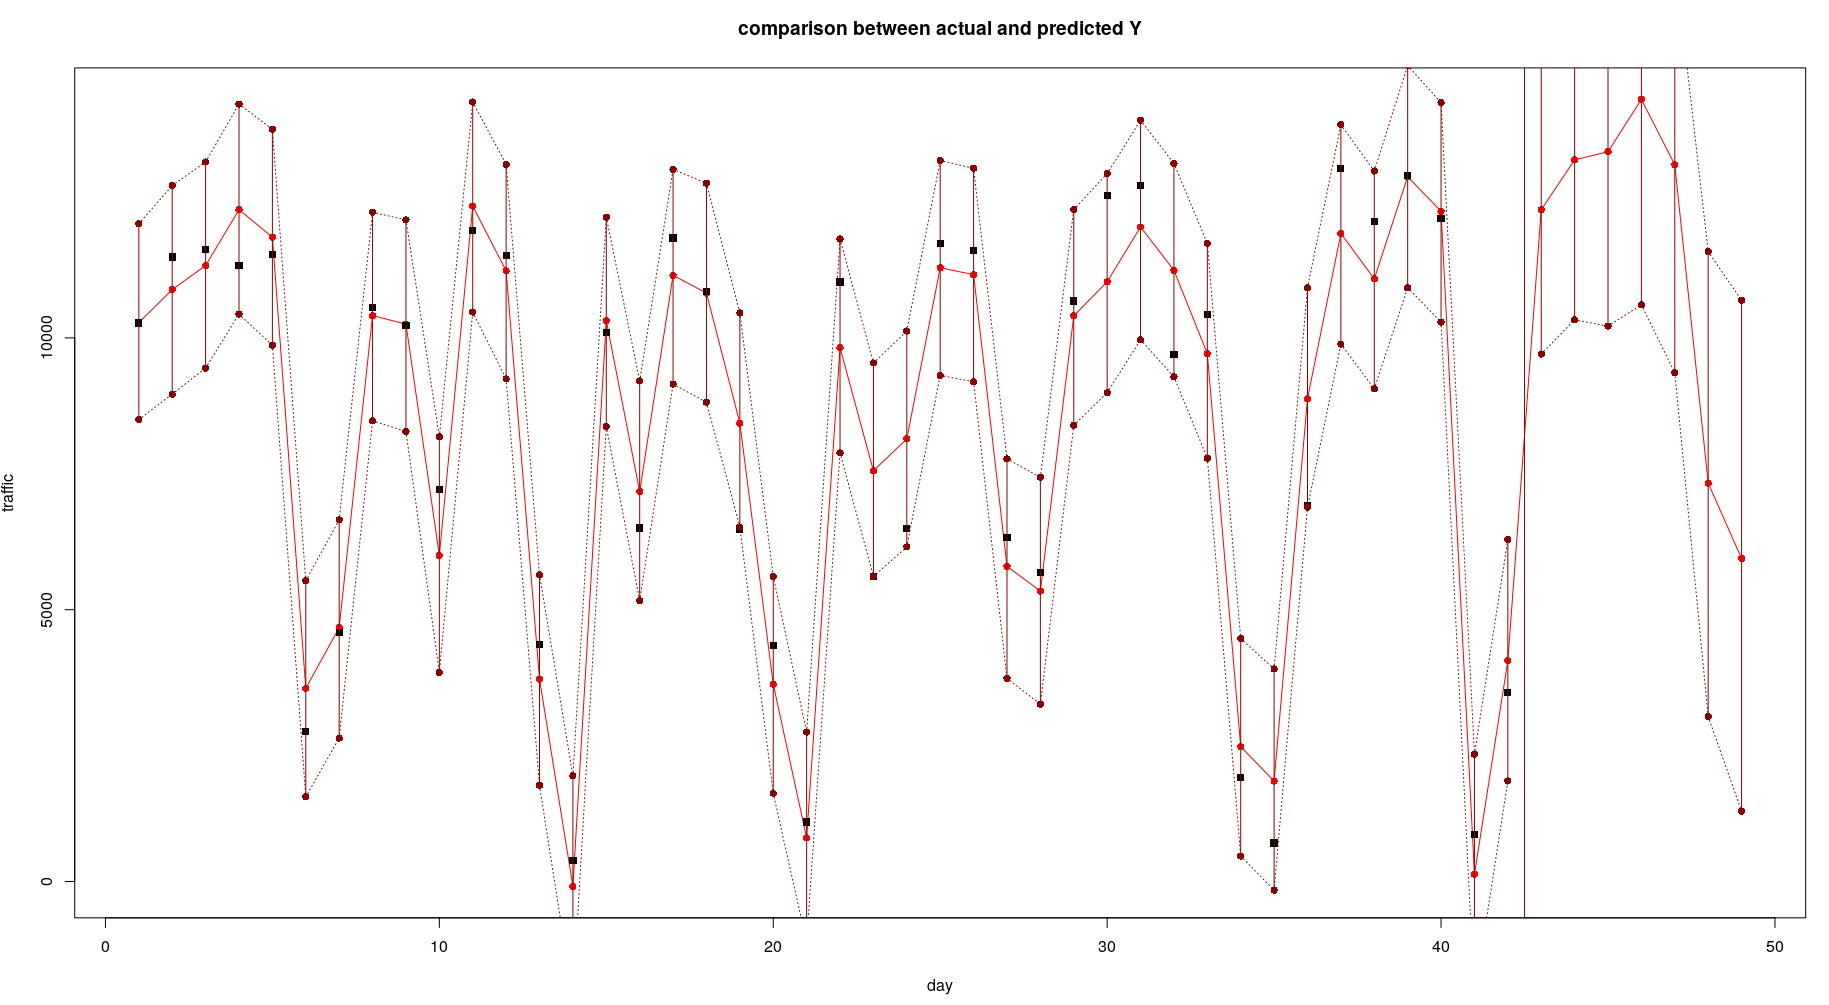
\includegraphics[width=150 mm]{pictures/m1_future.png}
	\caption{Present and future prediction according to the model}
	\label{fig:M1_future}
\end{figure}

\subsubsection{Standard with autoregression, without temperature}
Given the relative importance represented by temperature in our models, often resulting in a mere quite uniform vertical translation of the whole function, we can take into consideration its elimination from the set of regressors and a possible incorporation of its non-negative action in the trend. We will see what happens to the previous model under these modifications and discuss their worth. Just keep into account that the only difference with the previous model lies in term $ \boldsymbol{\beta}^T\mathbf{z} $ now reduced from $ (\beta_1+\nu_1w)z_1 + (\beta_2+\nu_2w)z_2$ to $(\beta+\nu w)z_1$.

\begin{figure}[H]
	\centering
	\includegraphics[width=46 mm]{pictures/m3_b1.png}
	\label{fig:M3_b1}
	\caption{Results produced by the model}
\end{figure}

\paragraph{Diagnostics} Boxplots are almost identical to the ones belonging to the previous model. The main difference can be seen in the 
expresion of the $ \tau $s. Indeed, as the picture shows, the variance $ \tau_1 $ of the output error seems to reach greater values than in the previous case (almost double), since the precision of the term appears halved. This is a negative factor: doubling the variance of the output entails a stronger difficulty of the model to capture the real behaviour of the structure, since, at least in priciple, a good model should have a $ \tau_1 $ as small as possible. To conclude the worth of MCMC chain is substantially identical to that of the previous model in all components, independently of temperature removal (which was, by the way, a hardly mixing regressor).


\paragraph{Results} The same can be said looking at the predicted time series, which appears qualitatively slightly more inaccurate (higher variability implies increased size of the credibility intervals). Note also that the trend has a more oscillating behaviour, this might indicate that the effect of temperature has been absorbed by this term, destibilizing it a bit. Bayesian residuals and predictive p-values are too similar with the previous case to be a direct matter of comparison. Also the estimated number outliers is always oscillating betwen two and three. Thus, it's better to entrust this role to other more effective strategies, like automatic evaluation procedures. We will discuss the results together with that of the robust model in the next paragraph.


\begin{figure}[H]
	\begin{subfigure}[H]{1\linewidth}
		\centering
\includegraphics[width=135 mm]{pictures/m3_p1.png}
\caption{Sum of trend (blue), periodicity (green), autoregression (yellow) and regression (red)}
\label{fig:M3_p1}
	\end{subfigure}
	\vfill
	\begin{subfigure}[H]{1\linewidth}
		\centering
\includegraphics[width=135 mm]{pictures/m3_p2.png}
\caption{90\% credibility intervals in dark red, in black the true responses $ y $}
\label{fig:M3_p2}
	\end{subfigure}%
	\caption{Results produced by the model}
\end{figure}

\subsubsection{Robust standard with autoregression model}
In order to better evaluate the worth of our original model it may seem wise to compare it with a more robust version, where the dependencies are fixed in way that each term of the trend and slope is made dependent not only on its past value (i.e current time), but also on some analogue days in the past. We can see a simple example that we tried to implement and simulate in the following, with hyperparameters fixed as in the previous models.

\begin{model} Robust corrected standard BSTS with autoregrssion
	\begin{equation*}
	\begin{aligned}
	&\textsc{Model}\\
	&Y_t = \mu_t + \gamma_t + \rho_t + \boldsymbol{\beta}^T\mathbf{z}_t + \tau_\epsilon^{-\frac{1}{2}}\tilde{\epsilon}_t\\
	&\mu_t = \mathcal{L}_t(\mu) + \mathcal{L}_t(\delta) +\tau_\eta^{-\frac{1}{2}}\tilde{\eta}_t\\
	&\delta_t = \mathcal{L}_t(\delta) + \tau_v^{-\frac{1}{2}}\tilde{v}_t\\
	&\gamma_t = \sum_{i=1}^{S-1}\gamma_{t+i-S} + \tau_w^{-\frac{1}{2}}\tilde{w}_t\\
	&\rho_t = \alpha\rho_{t-1} + \tau_u^{-\frac{1}{2}}\tilde{u}_t\\
	&\tilde{\epsilon}_t, \tilde{\eta}_t, \tilde{v}_t, \tilde{w}_t, \tilde{u}_t \overset{iid}{\sim} \mathcal{N}(0,1)\\
	\\
	&\textsc{Initial Conditions}\\
	&\mu_0 \sim \mathcal{N}(m, \tau_\eta)\quad \quad \quad \quad \quad\  m\ \ hpm\\
	&\delta_0 \sim \mathcal{N}(d, \tau_v)\quad \quad \quad \quad \quad \quad d\ \ \ hpm\\
	&\boldsymbol{\gamma}_{0:(2-S)} \sim \mathcal{N}_{S-1}(\mathbf{g}, \tau_w\mathbf{I})\quad\ \ \mathbf{g}\ \ hpm\\
	&\rho_0 \sim \mathcal{N}(r, \tau_u)\quad \quad \quad \quad \quad \quad \ r\ \ hpm\\
	\\
	\end{aligned}
	\qquad \qquad
	\begin{aligned}[c]
	&\textsc{Priors}\\
	&\boldsymbol{\beta} \sim \mathcal{N}_p(\mathbf{0}, \tau_b \mathbf{I})\ \ \quad \quad \quad \quad \quad \tau_b\ \quad \ hpm\\
	&\alpha \sim \mathcal{N}(a, \tau_a) \ \quad \quad \quad \quad \quad \quad a, \tau_a\ \ hpm\\
	&\tau_\epsilon \sim Unif(a_\epsilon, b_\epsilon)\quad\quad\ \quad \quad a_\epsilon, b_\epsilon\ \ hpm\\
	&\tau_\eta \sim Unif(a_\eta, b_\eta)\quad\quad\quad \quad a_\eta, b_\eta\ \ hpm\\
	&\tau_v \sim Unif(a_v, b_v)\quad\quad\quad \quad a_v, b_v\ \ hpm\\
	&\tau_w\sim Unif(a_w, b_w)\quad\quad\quad\ a_w, b_w\ \ hpm\\
	&\tau_u \sim Unif(a_u, b_u)\quad\quad\quad\quad a_u, b_u\ \ hpm\\
	&\\
	&\textsc{Operators}\\
	&\mathcal{L}_t(\cdot) = \frac{1}{2}(\cdot)_{t-1} + \frac{1}{3}(\cdot)_{t-S} +\frac{1}{6}(\cdot)_{t-2S}\\
	&\\
	&\textsc{Independence}\\
	&\{\tilde{\epsilon}_t, \tilde{\eta}_t, \tilde{u}_t, \tilde{w}_t, \tilde{v}_t, \mu_0, \delta_0, \boldsymbol{\gamma}_{0:(-S+2)}, \rho_0,\\ &\boldsymbol{\beta}, \alpha, \tau_\epsilon, \tau_\eta, \tau_v, \tau_w, \tau_u\}\\ &family\ of \independent real\ random\ variables\\
	&\\
	\end{aligned}
	\end{equation*}
\end{model}
\begin{figure}[H]
	\centering
	\includegraphics[width=150 mm]{pictures/m4_p1.png}
	\caption{Cumulative action of trend (blue), periodicity (green), autoregression (yellow) and regression (red) in robust model}
	\label{fig:M4_p1}
\end{figure}
\paragraph{Results}
It is possible to show that boxplots regarding this section are approximately similar to the ones without the presence of temperature within the regressors, i.e. stable, but with a lower precision on the output error. As always this might be considered a factor suggesting a worsening in the partition of uncertainty between state and output. But differently from the previous case, where the state is forced to oscillate too much for a lack of accuracy at local level, here the variation is due to an increased inability of the state (and in particular the trend-slope) to fit the fluctuations of the data. Indeed, as it can also be shown by the following picture there is a high risk of trend oversmoothing.
It has to be remarked that even though the number of outliers is unchanged from the previous models, the three "historical" outliers of the problem are even more uncapturated than in the previous cases. We are now going to discuss wich model among standard, robust and without temperature should be considered the best according to the criteria discussed in the previous section. Using the mean normalized residuals in time as an evaluation criterion the values are not varying too much, the smallest is reached for the standard model, hence it should be considered the best, at least according to this criterion. As for mean tail probabilities, the version without temperature seems slightly more accurate than the others (on average), however the difference with the standard is so close that we can still continue to prefer it, especially in light of the shape of the trend interpretation discussed before. Finally, since also the $ elpd_{loo} $ takes its maximum in correspondence of the standard model, so that we can agree about this being considered the best among the ones seen so far. As a further step, we will immediately ponder the elimination  of the autoregresive part, that we have seen being more a badly playing figurant rather than a protagonist.

\begin{table}[!htb]
		\centering
		\begin{tabular}{|c|c|c|c|}
			\hline
			& standard & no temperature & robust \\
			\hline
			Mean standardized residuals &$  0.5809041 $ & $  0.6066627 $ &$  0.6031869 $\\
			\hline
			Mean tail probabilities &$ 0.2979543 $ & $  0.298591 $ &$  0.2908414 $\\
			\hline
			$ elpd_{loo} $ &$ -362.6 $ & $  -365.4 $ &$  -364.1 $\\
			\hline
		\end{tabular}
\end{table}

\subsubsection{Standard (without autoregression)}
Just recall that removing autoregression from the state, has an immediate benefit: it simplifies the model and reduces the number of parameters to be estimated. Moreover, we have already discussed in the previous paragraphs how null is impact due to $ \rho $ - capturing just a small variability and having 0 mean - not to mention the irregularity of its companion coefficient $ \alpha $. According to an old motto: "the simplest, the best", we will now test the hypotheses $ \rho_t=0,\ \forall t $.

\begin{model} Corrected standard BSTS
	\begin{equation*}
	\begin{aligned}
	&\textsc{Model}\\
	&Y_t = \mu_t + \gamma_t + \boldsymbol{\beta}^T\mathbf{z}_t + \tau_\epsilon^{-\frac{1}{2}}\tilde{\epsilon}_t\\
	&\mu_t = \mu_{t-1} + \delta_{t-1} +\tau_\eta^{-\frac{1}{2}}\tilde{\eta}_t\\
	&\delta_t = \delta_{t-1} + \tau_v^{-\frac{1}{2}}\tilde{v}_t\\
	&\gamma_t = \sum_{i=1}^{S-1}\gamma_{t+i-S} + \tau_w^{-\frac{1}{2}}\tilde{w}_t\\
	&\tilde{\epsilon}_t, \tilde{\eta}_t, \tilde{v}_t, \tilde{w}_t, \overset{iid}{\sim} \mathcal{N}(0,1)\\
	\\
	&\textsc{Initial Conditions}\\
	&\mu_0 \sim \mathcal{N}(m, \tau_\eta)\quad \quad \quad \quad \quad\  m\ \ hpm\\
	&\delta_0 \sim \mathcal{N}(d, \tau_v)\quad \quad \quad \quad \quad \quad d\ \ \ hpm\\
	&\boldsymbol{\gamma}_{0:(2-S)} \sim \mathcal{N}_{S-1}(\mathbf{g}, \tau_w\mathbf{I})\quad\ \ \mathbf{g}\ \ hpm\\
	\\
	\end{aligned}
	\qquad \qquad
	\begin{aligned}[c]
	&\textsc{Priors}\\
	&\boldsymbol{\beta} \sim \mathcal{N}_p(\mathbf{0}, \tau_b \mathbf{I})\ \ \quad \quad \quad \quad \quad \tau_b\ \quad \ hpm\\
	&\tau_\epsilon \sim Unif(a_\epsilon, b_\epsilon)\quad\quad\ \quad \quad a_\epsilon, b_\epsilon\ \ hpm\\
	&\tau_\eta \sim Unif(a_\eta, b_\eta)\quad\quad\quad \quad a_\eta, b_\eta\ \ hpm\\
	&\tau_v \sim Unif(a_v, b_v)\quad\quad\quad \quad a_v, b_v\ \ hpm\\
	&\tau_w\sim Unif(a_w, b_w)\quad\quad\quad\ a_w, b_w\ \ hpm\\
	&\\
	&\\
	&\\
	&\textsc{Independence}\\
	&\{\tilde{\epsilon}_t, \tilde{\eta}_t, \tilde{w}_t, \tilde{v}_t, \mu_0, \delta_0, \boldsymbol{\gamma}_{0:(-S+2)}, \boldsymbol{\beta}, \tau_\epsilon, \tau_\eta, \tau_v, \tau_w, \}\\ &family\ of \independent real\ random\ variables\\
	&\\
	&\\
	\end{aligned}
	\end{equation*}
\end{model}

\begin{figure}[H]
	\centering
	\includegraphics[width=150 mm]{pictures/m5_p1.png}
	\caption{Cumulative action of trend (blue), periodicity (green)and regression (red) in robust model}
	\label{fig:M5_p1}
\end{figure}

Fixing hyperparameters as always, we can easily infer from boxplots that the model has reached a good level of stability even without the presence of the last type of error, moreover the magnitude among other terms is almost unchanged. A remark: note that the predictive power of the structure is almost identical to that with the autoregressive part. Indeed the number of data outliers with respect to the predictive distribution of $ y $ is always 3, the average Bayesian p-value is 0.2970371 and normalized residuals 0.5846875. These numbers suggest that the difference with the autoregressive state model is almost null. Not to mention the the $ elpd_{loo}=-362.4 $, even lower than its analogue with $ \rho $s. Summing up all evidence, and taking into account that this decision is also coherent with the will of avoiding an awfully behaving term with respect to the chain mixing and posterior appearence, there is a general ageement towards eliminating the additional autoregressive state. Let's try to understand why this term apears not relevant and give some suggestions about further directions of investigation concerning this problem.\\
\\
Fist of all, it's not likely the autoregression to be useless at all, but probably it should be considered in a different way: not as a long time running Markov chain, trained with global coeficients, but more as a mesoscale factor with pseudo-local coefficents. Indeed, just observe that predicting with our models there are some consecutive days where the forecasts are constantly overoptimistic or overpessimistic. This might be due to the presence of a local autoregression effect, deriving probably from an extended period of warmth or rain. However, if we try to collect these two types of effect together with a single autoregression coefficient, this property is obviously lost $ in\ toto $, since opposite terms cancel out. Substantially what we might propose for a future development is a sort of lower level connection  between the regresion part and the autoregression, in  order to define a more accurate way to incorporate positive/negative short-time feedbaks derived from iterated meteorological pheneomena. The idea is very appealing, but of difficult formulation and - even greater problem - needs lots data to be well trained.\\
\\
As a final comment, let us spend a few words on picture \ref{fig:pt}, in which we tested the stability of our prediction on already defined data. In this case, instead of exploiting all 42 days as training set for our Bayesian model, we decided to select just the first 35 and let the resulting ones (i.e. the last of 6 weeks) to be used as a test with which try out our paradigm's goodness of fit. As we can see results are neither perfect nor terrible. First of all, we have to admit that the size of $ 90\% $ prediction intervals is much larger than the one concerning the corresponding credibility intervals. Note that this happens beacause the standard deviation of the prediction densities is almost 1.5 the one of the confidence ones. This makes much simpler for observations to lie within these large boundaries. Nonetheles we can observe that all our data fit rather well inside these limits, even the datum about monday, which is quite difficult to be accepted even in the case where this element is given in he training set. However, the error appears rather systematic, namely we tend to understimate six times out of seven the actual value assumed by our data. Is this given by chance or it might be an hint suggesting us the need to revise a bit the way we estimate the trend? Given the small amount of data we have, it is quite impossible give an affordable answer to the question.

\begin{figure}[H]
	\centering
	\includegraphics[width=150 mm]{pictures/predicted_traffic.png}
	\caption{Predicted traffic with the model}
	\label{fig:pt}
\end{figure}

\subsubsection{Standard with rain mm}
As a final model let's consider a slight variation of the previous paradigm, where instead of a qualitative a priori scale for the rain we consider the mm registered on that day. This choice is not completely uncontroversial. In fact, as it might appear obvious, the exact amount of rain fallen daily is not something that can be known a priori when predictions are to be made, but only a posteriori, once the day is over. However, given the increased affordability of scientific tools able to predict with precision how much rainy a day will be, we can nonetheless try to see if this estimate may lead to more accuracy in the prediction or not. Note that the answer might not be so trivial, bacause even though having precise data may be better than relying on a qualitative scale, a big doubt is about how many people will even get in contact with them or make choices according to that knowledge. In principle, it is more likely for bike users to rely on pre-codified weather forecasts, which are - by construction - qualitative scales, often made by pictures and not by numbers. And even the perception of these pictures might be much different from the actual amount of rain that will fall. Moreover, another problem regards in which way to use the data provided by the mm. Difficultly we should add a linear regression proportional to these data, nor to their logarithm, probably something like a square root may perform better. However, the problem that lies in finding a typical dimension to be general enough and independent from the actual perception is rather difficult to be solved.  Not to mention that sometimes is not even the overall amount of rain which matters, but something like its distibution over the day: a strong storm may have less effect than a prolonged drizzle. Eventualy, all these long speeches just to state the obvious: there is no data format regarding weather conditions or forecasts that can be considered, a priori, the perfect regressor. Each case has to be studied singularly, and this is exactly what we will be doing now, with Bayesian tools.

\begin{figure}[H]
	\centering
	\includegraphics[width=60 mm]{pictures/m6_out.png}
	\caption{Outliers according to the model}
	\label{fig:M6_out}
\end{figure}

\paragraph{Results} In this case, due to the similarity with other models already seen, we only limit ourseleves to discuss in brief the results. Note that the diagnostics are pretty similar to the ones of subsections above, the only difference lies in the dimension of $ \tau_1 $ that is almost halved with respect to previous models (meaning double variance and hence double uncertainty). The model is indeed less capable of predicting the results as can be deduced from the $ elpd_{loo} $ equal to $ -372.3 $, mean predictive tails $ 0.2829 $ and mean Bayesian residuals $ 0.640  $ definitely worse than in the aforementioned paradigms. There is also an increase in the number of outliers that passes from 3 to almost 4-5, as can be seen from the picture \ref{fig:M6_out}.
Note that differences are not that dramatic since in the end BSTS structure always manages to find an equilibrium point in order to get a good compromise between structure and data. However - at least in this case - we can say that the tip of the balance is played by the precision $ \tau_1 $. As already remarked before, the role of this quantity is that of determining the variability of the output error. It is obvious that the dimension of this term is bound to be greater than that of the one concerning the state.
 
 \begin{figure}[H]
 	\centering
 	\includegraphics[width=150 mm]{pictures/m6_p1.png}
 	\caption{Confidence intervals are larger than in previous models}
 	\label{fig:M6_p1}
 \end{figure}

However, if a model doubles the center of its poterior distribution (i.e. its posterior median), this should lead us to consider the prediction less reliable. Just observe that having an inaccurate prediction is not a negative factor as a matter of priciple, because a phenomenon might be structurally fairly variable. Fortunately enough, if we have two ways to make analyses using mutually exclusive set of covariates and one performs better than the other, it appears quite reasonable to select the one that produces the smallest residual variability, and in this case we can follow this route to identify a preferable paradigm.
As a final comment let us strike a blow in defence of the models which have been considered suboptimal so far. Having to deal with very complicated structures where a lot of parameters have to be estimates, like in STS models, can be very difficult and there is always a strong risk of overfitting where the data are not excessively numerous. The Bayesian setting may somehow mitigate this problem, giving us a tool, the predictive distribution of the errors, to establish the accuracy of the different models. However it still remains evident that predictive power can't be estimated precisely with only 42 data. Hence all these discussions would be much more effective being able to test the results on a longer time span, or, at least, on multiple analogous time spans across different years.
 
 \subsection{Global model with time zones}
 The last BSTS model we want to present is a variation of the previous cases defined to capture the difference in time zones across various days. Note that the structures discussed so far have always had as main goal that of making inference about the overall amount of bikes running on the network in a certain day. The aim of this section is different. In the data preprocessing we got the chance to subdivide the overall traffic in four meaningful standard time zones: morning (6 a.m - 9 a.m), midday (10 a.m. - 3 p.m.), late afternoon (4 p.m. - 7 p.m.) and night (8 p.m. - 1 a.m). We are now going to make predictions dividing the flow in these groups, trying to fit an evolution of standard BSTS model without autoregression which suits well these separations.
 As a main modification, we will have to introduce a way to capture the flow of traffic within a certain day. This can be done in a rather easy way, exploiting the modularity of BSTS approach. As mentiond in the introduction, BSTS is able to support multiple periodicities within the same framework and this is exactly what can be turned in a strong advantage. Indeed, adding a second inner cycle covering a whole day, we can get the superposition of two loops and hence derive the output as sum of locally linear trend, a regression factor and these two effects. Note that in the following $ t $ will denote the day (ranging from 1 to 42) while $ h $ is the time fraction in $ 1:4=F $. $ S=7 $, as always, is the number of days in a week.
 
 \begin{model} Corrected standard BSTS with time zones
 	\begin{equation*}
 	\begin{aligned}
 	&\textsc{Model}\\
 	&Y_{F(t-1)+h} = \\&\quad\quad
 	\mu_{t} + \gamma_{t} + \chi_{F(t-1)+h} + \boldsymbol{\beta}^T\mathbf{z}_{th} + \tau_\epsilon^{-\frac{1}{2}}\tilde{\epsilon}_{F(t-1)+h}\\
 	&\mu_t = \mu_{t-1} + \delta_{t-1} +\tau_\eta^{-\frac{1}{2}}\tilde{\eta}_t\\
 	&\delta_t = \delta_{t-1} + \tau_v^{-\frac{1}{2}}\tilde{v}_t\\
 	&\gamma_t = \sum_{i=1}^{S-1}\gamma_{t+i-S} + \tau_w^{-\frac{1}{2}}\tilde{w}_t\\
 	&\chi_{F(t-1)+h} = \sum_{j=1}^{F-1}\chi_{F(t-1)+h+j-F} + \tau_u^{-\frac{1}{2}}\tilde{u}_{F(t-1)+h}\\
 	&\tilde{\epsilon}_{F(t-1)+h}, \tilde{\eta}_t, \tilde{v}_t, \tilde{w}_t, \tilde{u}_{F(t-1)+h} \overset{iid}{\sim} \mathcal{N}(0,1)\\
 	\\
 	&\textsc{Initial Conditions}\\
 	&\mu_0 \sim \mathcal{N}(m, \tau_\eta)\quad \quad \quad \quad \quad\  m\ \ hpm\\
 	&\delta_0 \sim \mathcal{N}(d, \tau_v)\quad \quad \quad \quad \quad \quad d\ \ \ hpm\\
 	&\boldsymbol{\gamma}_{0:(2-S)} \sim \mathcal{N}_{S-1}(\mathbf{g}, \tau_w\mathbf{I})\quad\ \ \mathbf{g}\ \ hpm\\
 	&\boldsymbol{\chi}_{0:(2-F)} \sim \mathcal{N}_{F-1}(\mathbf{c}, \tau_u\mathbf{I})\quad\ \  \mathbf{c}\ \ hpm\\
 	\\
 	\end{aligned}
 	\qquad \qquad
 	\begin{aligned}[c]
 	&\textsc{Priors}\\
 	&\boldsymbol{\beta} \sim \mathcal{N}_p(\mathbf{0}, \tau_b \mathbf{I})\ \ \quad \quad \quad \quad \quad \tau_b\ \quad \ hpm\\
 	&\tau_\epsilon \sim Unif(a_\epsilon, b_\epsilon)\quad\quad\ \quad \quad a_\epsilon, b_\epsilon\ \ hpm\\
 	&\tau_\eta \sim Unif(a_\eta, b_\eta)\quad\quad\quad \quad a_\eta, b_\eta\ \ hpm\\
 	&\tau_v \sim Unif(a_v, b_v)\quad\quad\quad \quad a_v, b_v\ \ hpm\\
 	&\tau_w\sim Unif(a_w, b_w)\quad\quad\quad\ a_w, b_w\ \ hpm\\
 	&\tau_u\sim Unif(a_u, b_u)\quad\quad\quad\ \ a_u, b_u\ \ hpm\\
 	&\\
 	&\\
 	&\\
 	&\\
 	&\\
 	&\\
 	&\textsc{Independence}\\
 	&\{\tilde{\epsilon}_t, \tilde{\eta}_t, \tilde{w}_t, \tilde{v}_t, \mu_0, \delta_0, \boldsymbol{\gamma}_{0:(-S+2)}, \boldsymbol{\chi}_{0:(2-F)},\\&\boldsymbol{\beta}, \tau_\epsilon, \tau_\eta, \tau_v, \tau_w, \tau_u \}\\ &family\ of \independent real\ random\ variables\\
 	&\\
 	&\\
 	\end{aligned}
 	\end{equation*}
 \end{model}

Just a little comment on this choice and possible variations: the idea of using two periodicities is rather simple and as we will see from the results, also pretty effective. A more refined strategy might be that of considering the presence of two distinct internal loops $ \phi $ and $ \psi $, the first only for weekdays and the second for weekends. This proposal meets quite well the graphs, since, as we will see from pictures, weekdays have a typical oscillating behaviour that priviledges the time slots concernig commuters from stations (i.e. working hours). Conversely, during the weekends, spare time hours are much more interested by traffic than in the previous cases. However the poor amount of data at our disposal makes infeasible to estimate these parameters alltogether, nonetheless we might consider this as a possible variant/improvement for our work. 

\paragraph{Hyperpameters}
The hyperparameters used in this model are substantially equivalent to the ones seen in the previous subsections, with some slight variations, starting from the regression part. Encouraged by the results discussed in the full-day case we kept track of both temperature and rain. Unfortunately, as already remarked above, the data at our disposal have a daily accuracy hence we were not able to get precise estimates for the single time slots using simply this information. Nonetheless the regression proved to be a fundamental factor also in this case. Concerning the structure of $ \boldsymbol{\beta}^T\mathbf{z} $, we opted for the following rule: $ \boldsymbol{\beta}^T\mathbf{z} = (\beta_1+\nu_1\mathbb{I}_{weekend}(t)+\xi_h)\cdot z_1(F(t-1)+h) + (\beta_2+\nu_2\mathbb{I}_{weekend}(t))\cdot z_2(F(t-1)+h)$, where $ \boldsymbol{\beta} $ is the common baseline for all days, $ \boldsymbol{\nu} $ is the particular action of weekends, and $ \boldsymbol{\xi} $ is the correction to the effect created by of rain given by the time slot (namely the correction will be less strong in hours where the traffic is weaker). Moreover $ \boldsymbol{\beta},\boldsymbol{\nu},\boldsymbol{\xi}\independent\mathcal{N}(0,\tau_*) $ and we use uninformative priors, indeed:

\begin{table}[!htb]
	\begin{subtable}{.5\linewidth}
		\centering
		\begin{tabular}{|c|c|c|c|c|c|}
			\hline
			& $ \tau_\epsilon $ & $ \tau_\eta $ &$  \tau_v $ & $ \tau_w $ & $ \tau_ u $\\
			\hline
			a &$  1\mathrm{e}{-7} $ & $  1\mathrm{e}{-5} $ &$  1\mathrm{e}{-5} $&$  1\mathrm{e}{-5} $&$  1\mathrm{e}{-5} $\\
			\hline
			b &$  1\mathrm{e}{-4} $ & $  1\mathrm{e}{-4} $ &$  1\mathrm{e}{-4} $&$  1\mathrm{e}{-4} $&$  1\mathrm{e}{-4} $\\
			\hline
		\end{tabular} 
	\end{subtable}%
	\begin{subtable}{.5\linewidth}
		\centering
		\begin{tabular}{|c|c|c|c|c|}
			\hline
			& $ \tau_\nu $ & $ \tau_\beta $ & $ \tau_\xi $ & $ d $\\
			\hline
			value &$  1\mathrm{e}{-5} $ & $  1\mathrm{e}{-5} $& $ 1\mathrm{e}{-5} $ & 0\\
			\hline
		\end{tabular} 
	\end{subtable} 
\end{table}

While $ \mu_0 $, $ \boldsymbol{\chi}_{0} $ and $ \boldsymbol{\gamma}_{0} $ are initialized using information coming form the frequentist stationarization. $ \mu_0 $ is the moving average divided by $ 4 $, same for the periodic component with respect to the moving period, while $ \chi $ follows as the difference in fluctuation averaged  along time slots (i.e. it is the average in time for each $ h $ of the difference between single $ y_{th} $ and moving average + period correspondig to that $ t $).

\paragraph{Diagnostics}
Here is a list of the most interesting diagnostics, from boxplots testifying the stability of the chain to more refined traceplots and distributions to show that posterior probabilities are regular enough in the model that we aim to evaluate. All the computations are done with a two chains 1,000,000 iterations structure, with 100 thinning and 10,000 burnin. These extremely huge numbers are necessary given the small amount of data and the need of decrease strongly autocorrelation.

\begin{figure}[H]
		\centering
		\includegraphics[width=100 mm]{pictures/taus.png}
		\caption{Boxplot of the $ \tau $s samples}
		\label{fig:taus}
\end{figure}

\begin{figure}[H]
	\begin{subfigure}[H]{0.50\linewidth}
		\centering
		\includegraphics[width=58 mm]{pictures/beta_1_2.png}
		\caption{Diagnostics for $ \beta_1 $ samples}
		\label{fig:beta_1_2}
	\end{subfigure}
	\hfill
	\begin{subfigure}[H]{0.50\linewidth}
		\centering
		\includegraphics[width=58 mm]{pictures/beta_2_2.png}
		\caption{Diagnostics for $ \beta_2 $ samples}
		\label{fig:beta_2_2}
	\end{subfigure}%
	\vfill
	\begin{subfigure}[H]{0.50\linewidth}
		\centering
		\includegraphics[width=58 mm]{pictures/nu_1_2.png}
		\caption{Diagnostics for $ \nu_1 $ samples}
		\label{fig:nu_1_2}
	\end{subfigure}
	\hfill
	\begin{subfigure}[H]{0.50\linewidth}
		\centering
		\includegraphics[width=58 mm]{pictures/nu_2_2.png}
		\caption{Diagnostics for $ \nu_2 $ samples}
		\label{fig:nu_2_2}
	\end{subfigure}%
	\vfill
	\begin{subfigure}[H]{0.50\linewidth}
		\centering
		\includegraphics[width=58 mm]{pictures/xi_1_2.png}
		\caption{Diagnostics for $ \xi_1 $ samples}
		\label{fig:xi_1_2}
	\end{subfigure}
	\hfill
	\begin{subfigure}[H]{0.50\linewidth}
		\centering
		\includegraphics[width=58 mm]{pictures/xi_2_2.png}
		\caption{Diagnostics for $ \xi_2 $ samples}
		\label{fig:xi_2_2}
	\end{subfigure}%
	\vfill
	\begin{subfigure}[H]{0.50\linewidth}
		\centering
		\includegraphics[width=58 mm]{pictures/xi_3_2.png}
		\caption{Diagnostics for $ \xi_3 $ samples}
		\label{fig:xi_1_3}
	\end{subfigure}
	\hfill
	\begin{subfigure}[H]{0.50\linewidth}
		\centering
		\includegraphics[width=58 mm]{pictures/xi_4_2.png}
		\caption{Diagnostics for $ \xi_4 $ samples}
		\label{fig:xi_2_4}
	\end{subfigure}%
\end{figure}

\begin{figure}
\begin{subfigure}[H]{0.50\linewidth}
	\centering
	\includegraphics[width=58 mm]{pictures/tau_4.png}
	\caption{Diagnostics for $ \tau_4 $ samples}
	\label{fig:tau_4}
\end{subfigure}
\hfill
\begin{subfigure}[H]{0.50\linewidth}
	\centering
	\includegraphics[width=58 mm]{pictures/tau_5.png}
	\caption{Diagnostics for $ \tau_5 $ samples}
	\label{fig:tau_5}
\end{subfigure}%
\end{figure}

\begin{figure}[H]
		\centering
		\includegraphics[width=58 mm]{pictures/tau_1.png}
		\caption{Diagnostics for $ \tau_1 $ samples}
		\label{fig:tau_1}
\end{figure}%

As it can be deduced from pictures the shapes of all the regression coefficents are definitely good: traceplots are fat enough and autocorrelation is kept under control, at least besides $\beta_2$ case which has been proved being erratic also in the previous subsections. Note in particular how number 0 dwells inside almost all the intervals, however it is evident that mostly of the cases hypotheses of the type $ coefficient=0 $ are very far from being acceptable. These results are a nasty consequence of the high uncertainty due to the lack of data. It is obvious that in a richer context, having much more data at our disposal, not only the distribution of these terms would be esimated with increased accuracy, but probably also the variability of parameters would be shrunk. Finally, observe the good shape of $ \tau_1 $ diribution: weak autocorrleation and good gamma-like profile testifies having reached a positive compromise for the value. Conversely $\tau_4$ and $\tau_5$ densities are fairly more biased towards one extremum of the interval, showing that we might take into account enlarging the space at their disposal. However, as it can be deduced form pictures, the distribution tends to assume larger values and not smaller. This is a positive factor, indeed it entails that we are underestimating a bit the precision, which is surely less damaging than overestimating it for predictive purposes. Nonetheless, as a future improvement of our model, we might try to look for better upper/lower limits where to encompass the single precisions in order to get the best possible posterior probabilities, both distributed as pseudo-gammas and well centered in the predefined intervals, yet without letting the dynamics to explode and collect all of the uncertainty in the observation error.

\paragraph{Results}
Figure \ref{fig:time series} shows the results of the analysis: in black we have the real observations, in red - linked by another line - our best prediction according to the mean squared error (posterior mean of $ y $). As we can see the lines are pretty much smilar and show most of the differences in days where there are strong rainy phenomena centered in a few hours of the day, for which we can only guess daily information irrespectively of intensity and duration. Moreover, it should be noted the ability of the structure to capture both weekdays an weekends, as shown by the confidence bars with which is endowed the mean line. However, the most interesting fact is given by the capability, not only to catch the real observations within credibility intervals, but also to follow the behaviour among several hours of the day: i.e. the model does not only appear locally reliable, but most of the times is also capable of predicting the slope between two consecutive observations (i.e if in the next time zone values will be higher or lower than the present ones). This is fundamental for strategies of adaptive control that try to follow the daily dynamics of the process in order to correct $ in\ medias\ res $ the possible shortages which may happen in the net, at least from a global viewpoint.

\begin{figure}[H]
	\centering
	\includegraphics[width=150 mm]{pictures/Time_series.png}
	\caption{Global time series per slot}
	\label{fig:time series}
\end{figure}%



\chapter{Network model}
In this chapter we propose possible models to describe the "flux" of bicycle in clusters of stations. Dividing the stations in clusters as pre-processing with a modified version of the DBSCAN algorithm, for every cluster the aim is to model the number of bicycles arriving and departing at stations belonging to the cluster: respectively $N^{IN}$ and $N^{OUT}$ in a certin time interval; we keep the division in days and time phases used in the BSTS. In this way the data are positive counts and the proposed models are \emph{Bivariate Poisson Two-Way Mixed GLMMs}.\\
\\
For the rest of this chapter the $i$ index will distinguish the cluster, $t$ will be used for weekend and weekdays, and $h$ for the time phases of the day. And thus $i \in 1,...,N\_nodes$, $t = 1,2$ and $h = 1,...,H$. We will use the index $u$ to distinguish between the different data points: for example if the third row of the dataset ($u=3$) belongs to a weekend it will be indicated as $t(u)=2$; in this way two data points will have the same distribution (covariates notwithstanding) if $h(u_1) = h(u_2)$ and $t(u_1)=t(u_2)$. In all computations $H=4$ and the time phases are the same used for the BSTS model.
The only two covariates that we will use are a dummy for the rain and the mean temperature for the day.
\section{Preprocessing}
As a raw dataset in the network model we used the following simplified tables, one for the $N^{IN}$ and one for the $N_{OUT}$. On the columns there are the nodes (clusterized stations) and on the rows the evolving time with row index $u$. Clearly $h(u) = u \mathrm{mod} H$ and the belonging to weekends can be also extracted from $u$. We also wondered on the possible correlation between $N^{IN}$ and $N^{OUT}$ of the same node and time phase. 

\section{The Likelihood}
If we fix the indexes the random variables $(N^{IN}_{ith}, N^{OUT}_{ith})$ are	correlated. Therefore we decide to model them with a \emph{Bivariate Poisson}.
\subsection{Bivariate Poisson}
We say $(Y_1,Y_2) \sim \mathrm{BPo}(\lambda_0, \lambda_1, \lambda_2)$ if:
\begin{equation}
\begin{cases}
Y_j = X_0 + X_j \quad j = 1,2\\
X_j \sim \mathrm{Po}(\lambda_j) \quad j = 0,1,2
\end{cases}
\end{equation}
With the convention that $\mathrm{Po}(0) = \delta_0$

\textbf{Properties:}
\begin{itemize}
	\item Marginally $Y_j \sim \mathrm{Po}(\lambda_0 + \lambda_j)$
	\item $\mathrm{Cov}(Y_1, Y_2) = \mathrm{Var}(X_0) = \lambda_0$
	\item $\rho_{1,2} = \frac{\lambda_0}{\sqrt{(\lambda_1 + \lambda_0)(\lambda_0 + \lambda_2)}}$
	\item The joint density is:
	$$\mathbb{P}(Y_1 = h, Y_2 = k) = e^{-(\lambda_0 + \lambda_1 + \lambda_2)}\frac{\lambda_1^h}{h!}\frac{\lambda_2^k}{k!}\sum_{l = 0}^{min(h,k)}{h\choose l}{k\choose l}l!(\frac{\lambda_0}{\lambda_1\lambda_2})^l$$
\end{itemize}
So $(N^{IN}_{it(u)h(u)}, N^{IN}_{it(u)h(u)}) \sim \mathrm{BPo}(\lambda^{(0)}_{it(u)h(u)}, \lambda^{(1)}_{it(u)h(u)}, \lambda^{(2)}_{it(u)h(u)})$ and the parameters of the model then are $(\lambda^{(0)}_{ith}, \lambda^{(1)}_{ith}, \lambda^{(2)}_{ith})$ and we will use for each of the three parameters the same hierarchical model.
\subsection{Zero Inflated Poisson}
We decided for a simple Poisson and not for a Zero Inflated Poisson for a purely computational reason, unfortunately the approximation revealed to bee too imprecise: the model fail to predict many zeros.

\begin{equation}
\begin{cases}
Y_j = \Gamma_j\delta_0 + (1-\Gamma_j)(X_0 + X_j) \quad j = 1,2\\
X_j \sim \mathrm{Po}(\lambda_j) \quad j = 0,1,2 
\end{cases}
\end{equation}

And implement a probit or logit link function for the $\Gamma_j$ parameters.

\section{Generalized Linear Two-Way Mixed Model}
As link function we choose the logarithm as is usual for a Poisson model. We deal with the division in weekdays/weekend and in the time phases in a similar way as a \emph{two-way ANOVA}, that is we consider the effect independent and sum the contributions. 

$$\gamma_{th}\cdot\mathbf{x} \rightarrow (\alpha_{t} + \beta_{h})\cdot\mathbf{x}$$

Conceptually this means that the effects influence the $\lambda$ parameter independently and there is a superposition of the effects of weekend and of the time phase.

Last we differentiate between two ways to deal with the nodal effect. 

\subsection{Offset model}
Taking inspiration from rate models with offsets we model the node effect as a multiplicative element that describes the size both in number of station per cluster and average number of travels. %Add more here as a description

\begin{equation}
\begin{cases}
\log(\lambda^{(j)}_{ith}) = (\boldmath{\theta^{(j)} +  \alpha^{(j)}_{t} + \beta_{h}^{(j)})}\cdot\mathbf{x} + \log(O_i)\\
\theta^{(j)}|a,B \stackrel{iid}{\sim} \mathcal{N}(a,B)\\
\alpha_{t}^{(j)}|\Sigma^{(j)} \stackrel{iid}{\sim} \mathcal{N}(0, \Sigma)\\
\beta_{h}^{(j)}|\Omega^{(j)} \stackrel{iid}{\sim} \mathcal{N}(0, \Omega)\\
a \sim \mathcal{N}(a_0, A_0)\\
B \sim invWishart(B_0, p+1)\\
\Sigma, \Omega \stackrel{iid}{\sim} invWishart(C_0, p+1)

\end{cases}
\end{equation}

%Riprendi come da slides di bayesiana il ruolo del mixed

There is the problem of deciding the offsets $O_i \in \mathbb{R}^+$, which give a measure of the "size" of the cluster both in number of stations and in bicycle traffic. For our computation we decided on a somehow suboptimal choice: 
$$O_i = \mathrm{Avg}(N^{IN}_i + N^{OUT}_i)$$

The offset is the average of traffic in the cluster, this creates a sort of circular dependency where we use the data to fit the data. We mitigated this by taking the average only on the first third of the dataset. In a real application one could divide the period in two, one to compute the offsets and the other to fit the model. We decided against this because the number of data points provided is already small.

\subsection{Model with parametric offsets (PO model)}
While we considered the offsets known in the previous model, we now group them with the other parameters.

\begin{equation}
\begin{cases}
\log(\lambda^{(j)}_{ith}) = (\boldmath{\theta^{(j)} +  \alpha^{(j)}_{t} + \beta_{h}^{(j)})}\cdot\mathbf{x} + \Phi_i\\
\theta^{(j)}|a,B \stackrel{iid}{\sim} \mathcal{N}(a,B)\\
\alpha_{t}^{(j)}|\Sigma^{(j)} \stackrel{iid}{\sim} \mathcal{N}(0, \Sigma)\\
\beta_{h}^{(j)}|\Omega^{(j)} \stackrel{iid}{\sim} \mathcal{N}(0, \Omega)\\
\Phi_i \stackrel{iid}{\sim} \mathcal{N}(\Phi_0, F_0)\\
a \sim \mathcal{N}(a_0, A_0)\\
B \sim invWishart(B_0, p+1)\\
\Sigma, \Omega \stackrel{iid}{\sim} invWishart(C_0, p+1)

\end{cases}
\end{equation}

Where the $\Phi_i \in \mathbb{R}$ take the role of $\log(O_i)$. The implicit belief of the model is that the $\Phi_i$, taking the role of a "size" parameter, does not depend on $j$; that is it has the same effect on both the inward and outward flux and their correlation. In this way it has the exact same role of the offsets and we will be able to compare the two.

\section{Computation of the posterior with JAGS software}
We used the package rjags to sample from the posterior of the $(\alpha_{t}^{(j)}, \beta_{h}^{(j)}, \theta^{(j)}, \Phi_i)$ parameters. Both models are computationally heavy, for this reason we had to limit the number of chains to 3 with 10000 iterations for the adaptation, 19000 for the burn-in and only 1000 effective sampling iterations, taken one every 10.\\

It's important to notice that not unlike a two-way ANOVA the models are not identifiable with respect to all parameters. Indeed only the sum $(\boldmath{\theta^{(j)} +  \alpha^{(j)}_{t} + \beta_{h}^{(j)})}$ with $t,h$ fixed has a meaning in itself. 

%%Add pic of the effect of summing the parameters (less important)

Even taking this into account, the results are unsatisfactory: in particularly regarding the adaptation, with the three chains stabilizing on three different values. Moreover the autocorrelation is too high in the offsets model, while being more acceptable in the PO model. \\

\begin{figure}[H]
	\begin{subfigure}[H]{.5\linewidth}
		\centering
		\includegraphics[width=70 mm]{pictures/posterior_off.png}
		\caption{For the offsets model}
		\label{fig:post_off}
	\end{subfigure}
	\hfill
	\begin{subfigure}[H]{.5\linewidth}
		\centering
		\includegraphics[width=70 mm]{pictures/posterior_nbn.png}
		\caption{For the PO model}
		\label{fig:post_nbn}
	\end{subfigure}%
	\caption{Results produced by the model}
\end{figure}


The predictiveness of both models is quite bad, with more than half of the data outside of their 95\% predictive intervals.

\begin{center}
	\begin{tabular}{ |c|c|c| } 
		\hline
		& $N^{IN}$ & $N^{OUT}$ \\ 
		\hline
		Offsets & 41.0\% & 62.2\% \\ 
		PO & 39.7\% & 38.6\% \\ 
		\hline
	\end{tabular}
\end{center}

Example of a simple table


We believe it might be because the JAGS chain could not reach stationarity, unfortunately we could run the chain for longer due to the computations being too time consuming. \\

\begin{figure}[H]
	\centering
	\includegraphics[width=150 mm]{pictures/cadorna_nin.png}
	\caption{}
	\label{fig:network_pred}
\end{figure}

There are also other possibilities: inspecting the plot \ref{fig:network_pred} of the prediction intervals we notice that there are two main categories of data points that the model systematically forecasts erroneously. The first are the zeros, which are more common in small nodes. The second case are "counter-nodes", clusters that behave in contrast with the others. For examples clusters near a big train station will see a net outward flux during the morning when commute workers leave the station, while other stations see a net inward flux of the same people arriving. Considering this, a possible generalization would be to employ a Zero Inflated Poisson likelihood and adding a two groups mixture effect of the time phase in the node $\beta_{t,i}$. 

\section{A final spatial model}
As a last possible presented model, let us discuss the following spatial structure that, even though too heavy to be developed and run in a small amount of time, might provide a good baseline for the investigation of some more advaced robust methods exploiting the graph structure of Milan BikeMi network of stations. The idea behind this structure is substantially that of mixing the BSTS approach with a loglinear model linking the evolution for the $ N_{in} $ and $ N_{out} $ through the iterative action of the whole graph in past times. The dynamic developement clearly makes the structure more robust (since we can always mitigate an extreme prediction using the effect of previous terms), but computationally inefficient (this might be a possible strong margin of improvement).\\
\\
Instead of modeling a bivariate Poisson through a fictitious common covariance term, with this approach we put the dependence at lower level still trying to  exploit the graph structure. We divide the nodes into $M$ groups. Notation: $ g(i) $ will denote the cluster of node $ i $ (classified through a mixture $ \delta(i) $ attribution variable), $ w(t) $ means if day $ t $ is weekend or weekday (mixed effect component).

\begin{model} Mixed loglinear-BSTS\\
\begin{equation*}
\begin{aligned}
&\textsc{Model}\\
&(N^{IN}, N^{OUT})_{ith}\sim Zip(\pi_{g(i)},\lambda_{ith}^{IN})\otimes Zip(\pi_{g(i)},\lambda_{ith}^{OUT})\\
&\log(\lambda^{j}_{ith}) = \mu^{j}_{ith}+\boldsymbol{\beta}^j_{g_iw_th}\mathbf{z}_t + \epsilon_{ith}^j\\
&\mu_{ith}^{IN} = \frac{1}{2} \mu^{IN}_{i(t-S)h} + \frac{1}{2} \frac{\sum_{j \in \mathcal{N}} \phi^{IN}_{ij}\mu_{jt(h-1)}^{OUT}}{\sum_{j \in \mathcal{N}} \phi^{IN}_{ij}}\\
&\mu_{ith}^{OUT} = \frac{1}{2} \mu^{OUT}_{i(t-S)h} + \frac{1}{2} \frac{\sum_{j \in \mathcal{N}} \phi^{OUT}_{ij}\mu_{jth}^{IN}}{\sum_{j \in \mathcal{N}} \phi^{OUT}_{ij}}\\
\end{aligned}
\qquad \qquad
\begin{aligned}[c]
&\textsc{Priors}\\
&\pi_{g(i)} \sim Be(p_{g(i)})\\
&\boldsymbol{\beta} \sim \mathcal{N}(\mathbf{0},\boldsymbol{\Sigma})\\
&\mathbf{\delta}_i \sim \mathrm{Dir}(a_1,...,a_M)
\end{aligned}
\end{equation*}
\end{model}

$ \phi_{ij}^* $ is a deterministic coefficient that takes into account both the distace of node $ j $ from $ i $ and the magnitude (IN or OUT) of the node $ j $, for instance we might select $ \phi_{ij}^*=\frac{s^*_j}{d_{ij}} $ where $ d_{ij} $ is the distance between node $ i $ and $ j $ and $ s_j^* $ is the (inner or outer) strength of $ j $. $ p_{g(i)} $ are also hyperparameters and their value is in (0,1), we can suppose a non-informative prior for vector $ \mathbf{p} $, or put all the coefficients to the same value. Finally, $ \boldsymbol{\delta} $ is the attribution parameter, that links each node to its cluster. We can suppose a Dirichlet prior for it, endowed with some uninformative parameter $ \mathbf{a} $. 

\appendix
\chapter{Model full conditionals}
\begin{lemma} Identification of a Markov chain\\
	Let $ \mathbf{X}_0 $ be a random vector with values in a set $ I^k $. Let $ \{\mathbf{Z}_n\}_{n\in\mathbb{N}_0}$ be a sequence
	of random vectos with values in a set $ \Xi^h $, $ \mathbf{X}_0 $ and $ \{\mathbf{Z}_n\}_{n\in\mathbb{N}_0}$ are independent.
	Suppose we are given a function
	$ F : I^k \times \Xi^h \rightarrow I^k $
	and define inductively
	$ \mathbf{X}_{n+1} := F (\mathbf{X}_n , \mathbf{Z}_{n+1} ) $, 
	$ \forall n \in \mathbb{N}_0 $.
	We suppose moreover that
	\begin{enumerate}
	\item $ \forall  n\in\mathbb{N}_0, \ \mathbf{k}, \mathbf{k}_{n-1} , \dots \mathbf{k}_1 \in \Xi^h,\ \mathbf{i}, \mathbf{i}_0 \in I^k:\\\ 
	\mathbb{P} (\mathbf{Z}_{n+1} = \mathbf{k}|\mathbf{X}_n = \mathbf{i}, \mathbf{Z}_{n-1} = \mathbf{k}_{n-1} , \mathbf{Z}_{n-2} = \mathbf{k}_{n-2} ,\dots, \mathbf{Z}_1 = \mathbf{k}_1 , \mathbf{X}_0 = \mathbf{i}_0 )
	=\\ \mathbb{P} (\mathbf{Z}_ {n+1} = \mathbf{k}|\mathbf{X}_n = \mathbf{i})$;
	\item $ \forall  n\in\mathbb{N}_0,\ \mathbf{k}\in \Xi^h,\ \mathbf{i} \in I^k:\ 
	\mathbb{P} (\mathbf{Z}_{n+1} = \mathbf{k}|\mathbf{X}_n = \mathbf{i}) = \mathbb{P} (\mathbf{Z}_1 = \mathbf{k}|\mathbf{X}_0 = \mathbf{i})$
\end{enumerate}
	Then the process $\{\mathbf{X}_n\}_{n\in\mathbb{N}}$ is an homogeneous Markov chain.
\end{lemma}
\begin{prop} Factorization of the joint density\\
	With respect to model 1:
	\begin{enumerate}
		\item $ \{\rho_t\}|\alpha, \tau_u $ is an homogeneous Markov chain;
		\item $ \{\boldsymbol{\gamma}_{t:t-S+1}\}|\tau_w $ is a S-dimensional homogeneous Markov chain;
		\item $ \{[\mu_t, \delta_t]^T\}|\tau_\eta, \tau_v $ is a 2-dimensional homogeneous Markov chain,  $ \{\delta_t\}|\tau_v $ is a Markov chain.
		\item $ \mathcal{L}(\mathbf{Y}, \boldsymbol{\mu}, \boldsymbol{\delta}, \boldsymbol{\gamma}, \boldsymbol{\rho}, \boldsymbol{\beta}, \alpha, \boldsymbol{\tau})  =\\  \prod_{i=1}^{n} \mathcal{L}(Y_i,| \mu_i,\gamma_i, \rho_i, \boldsymbol{\beta}, \tau_\epsilon)\mathcal{L}(\mu_i|\mu_{i-1}, \delta_{i-1},\tau_\eta)\mathcal{L}(\delta_i| \delta_{i-1},\tau_v)\mathcal{L}(\gamma_i| \boldsymbol{\gamma}_{(i-S+1):(i-1)}, \tau_w)\cdot\\\mathcal{L}(\rho_i|\rho_{i-1},\tau_u, \alpha)\mathcal{L}(\mu_0), \mathcal{L}(\delta_0), \mathcal{L}(\gamma_{(-S+2):0}) \mathcal{L}(\rho_0), \mathcal{L}(\boldsymbol{\beta}), \mathcal{L}(\alpha), \mathcal{L}(\tau_\epsilon)\mathcal{L}(\tau_\eta)\mathcal{L}(\tau_v)\mathcal{L}(\tau_w)\mathcal{L}(\tau_u)$
	\end{enumerate}
\end{prop}
\begin{proof}
	Following the order.
	\begin{enumerate}
		\item From the previous lemma, $ I=\Xi= \mathbb{R}\,\ F(x,z) = \alpha x + z $, the increments $ Z_n = \rho_n-\alpha\rho_{n-1} $ are independent w.r.t. $ \rho_0 $ and among themselves, thus the first requirement holds. By the identical distribution of the increments also the second condition is met.
		\item Same as before but, $ I=\mathbb{R}^S,\ \Xi= \mathbb{R}\,\ F(x,z) = [<\mathbf{x}, rep(-1,S-1)> + z, x_1, \dots, x_{S-1}]^T $, the increments $ Z_n = \gamma_n-\sum_{i=1}^{S-1}\gamma_{n+i-S} $ are independent w.r.t. $ \{\boldsymbol{\gamma}_{S-2:1}\} $ and among themselves, hence the first condition holds, the identical distribution of the increments implies the second.
		\item To see the 2D result, $ I^2=\Xi^2= \mathbb{R}^2\,\ F(\mathbf{x},\mathbf{z}) = [x1+x2,x2]^T + \mathbf{z}$  Vector $ \mathbf{X}_n = [\mu_n, \delta_n] $, with increments $ Z_n \overset{iid}{\sim} \mathcal{N}_2(\mathbf{0}, diag(\tau_\eta, \tau_v)) $ that are independent w.r.t. $ \{\mathbf{X}_0\} $ and i.i.d. among themselves, thus both conditions are met. We can repeat the same arguments taking $ I=\Xi= \mathbb{R}$ and $ X_n=\delta_n $ with $ Z_n \overset{iid}{\sim} \mathcal{N}(0,\tau_v) $, independent from $ \delta_0 $ for the first marginal result.
	
\item The idea behind the factorization is that of first identifying the dependece between one instant and the previous times and then exploiting the hierarchy to go deep in the dependece tree. Indeed:\\
$\mathcal{L}(\mathbf{Y}, \boldsymbol{\mu}, \boldsymbol{\delta}, \boldsymbol{\gamma}, \boldsymbol{\rho}, \boldsymbol{\beta}, \alpha, \boldsymbol{\tau})  =\\  \prod_{i=1}^{n}\mathcal{L}(Y_i, \mu_i, \delta_i, \gamma_i, \rho_i, | \mathbf{Y}_{1:(i-1)}, \boldsymbol{\mu}_{0:(i-1)}, \boldsymbol{\delta}_{0:(i-1)}, \boldsymbol{\gamma}_{(-S+2):(i-1)}, \boldsymbol{\rho}_{0:(i-1)}, \boldsymbol{\beta}, \alpha, \boldsymbol{\tau})\cdot\\
 \mathcal{L}(\mu_0), \mathcal{L}(\delta_0), \mathcal{L}(\gamma_{(-S+2):0}) \mathcal{L}(\rho_0), \mathcal{L}(\boldsymbol{\beta}), \mathcal{L}(\alpha), \mathcal{L}(\tau_\epsilon)\mathcal{L}(\tau_\eta)\mathcal{L}(\tau_v)\mathcal{L}(\tau_w)\mathcal{L}(\tau_u)$.\\
Where we can write $ \forall i \in 1:n $:\\
$\mathcal{L}(Y_i, \mu_i, \delta_i, \gamma_i, \rho_i, | \mathbf{Y}_{1:(i-1)}, \boldsymbol{\mu}_{0:(i-1)}, \boldsymbol{\delta}_{0:(i-1)}, \boldsymbol{\gamma}_{(-S+2):(i-1)}, \boldsymbol{\rho}_{0:(i-1)}, \boldsymbol{\beta}, \alpha, \boldsymbol{\tau}) =\\
\mathcal{L}(Y_i,| \mathbf{Y}_{1:(i-1)}, \boldsymbol{\mu}_{0:i}, \boldsymbol{\delta}_{0:i}, \boldsymbol{\gamma}_{(-S+2):i}, \boldsymbol{\rho}_{0:i}, \boldsymbol{\beta}, \alpha, \boldsymbol{\tau})\cdot\\
\mathcal{L}(\mu_i, \delta_i, \gamma_i, \rho_i| \mathbf{Y}_{1:(i-1)}, \boldsymbol{\mu}_{0:(i-1)}, \boldsymbol{\delta}_{0:(i-1)}, \boldsymbol{\gamma}_{(-S+2):(i-1)}, \boldsymbol{\rho}_{0:(i-1)}, \boldsymbol{\beta}, \alpha, \boldsymbol{\tau})$\\
Let's make some remarks:
\begin{itemize}
	\item The nature of some middle terms, $ \forall t \in \mathbb{N}_0 $:
	\begin{enumerate}
		\item $\delta_t = \delta_0 + \frac{1}{\sqrt{\tau_v}}\sum_{k=1}^{t}\tilde{v}_t$, depends on $ \delta_0, \tau_v, \tilde{\boldsymbol{v}}_{1:t} $
		\item $\mu_t = \mu_0 + \delta_{t-1} \frac{1}{\sqrt{\tau_\eta}}\sum_{k=1}^{t}\tilde{\eta}_t$, depends on $ \delta_0, \mu_0, \tau_v, \tau_\eta, \tilde{\boldsymbol{v}}_{1:(t-1)} \tilde{\boldsymbol{\eta}}_{1:t}$
		\item  $\gamma_t = f(\boldsymbol{\gamma}_{0:-(S+2)},\tilde{\mathbf{w}}_{1:t}, \tau_w)$
		\item $\rho_t = g(\rho_0,\tilde{\mathbf{u}}_{1:t}, \tau_u, \alpha)$
	\end{enumerate}
	Hence, by constructions the sequences $ (\boldsymbol{\mu}, \boldsymbol{\delta}),\boldsymbol{\rho}$ and $ \boldsymbol{\gamma} $ are independent.
	\item Notice moreover that conditioning with $ \mathbf{Y}_{1:(i-1)} $ can be dropped in both the cases.\\
	Indeed, $ \forall j \in 1:i $, $ Y_j  = \mu_j+ \gamma_j +\rho_j + \boldsymbol{\beta}\mathbf{z}_j + \frac{1}{\sqrt{\tau_\epsilon}}\tilde{\epsilon}_j$, where $\tilde{\epsilon}_j \overset{iid}{\sim}\mathcal{N}(0,1)  $. Hence, conditioning with all the rest $ Y_i = f(\tilde{\epsilon}_i) $ and $\mathbf{Y}_{1:(i-1)} = g(\tilde{\boldsymbol{\epsilon}}_{1:(i-1)} ) $, that are independent as functions of independent terms, which implies that we can drop the conditioning in the first term of the product. The second case is analogous but we have to use the fact that $[\mu_i, \delta_i, \gamma_i, \rho_i]^T = h(\tilde{\eta}_i, \tilde{v}_i, \tilde{u}_i, \tilde{w}_i) $ once the rest is fixed, that are independent from $ \tilde{\epsilon}_i $.
\end{itemize}

Entering in a deeper factorization:
\begin{itemize}
	\item Using independence $ \mathcal{L}(\mu_i, \delta_i, \gamma_i, \rho_i| \boldsymbol{\mu}_{0:(i-1)}, \boldsymbol{\delta}_{0:(i-1)}, \boldsymbol{\gamma}_{(-S+2):(i-1)}, \boldsymbol{\rho}_{0:(i-1)}, \boldsymbol{\beta}, \alpha, \boldsymbol{\tau}) = \\\mathcal{L}(\mu_i, \delta_i, | \boldsymbol{\mu}_{0:(i-1)}, \boldsymbol{\delta}_{0:(i-1)}, \tau_\eta, \tau_v)\mathcal{L}(\gamma_i| \boldsymbol{\gamma}_{(-S+2):(i-1)}, \tau_w)\mathcal{L}(\rho_i| \boldsymbol{\rho}_{0:(i-1)}, \alpha, \tau_u)$: 
	\begin{enumerate}
		\item $\mathcal{L}(\mu_i, \delta_i, |\boldsymbol{\mu}_{0:(i-1)}, \boldsymbol{\delta}_{0:(i-1)}, \tau_\eta, \tau_v) \overset{MC}{=}\mathcal{L}(\mu_i,\delta_i|\mu_{i-1}, \delta_{i-1},\tau_\eta, \tau_v) =\\ \mathcal{L}(\mu_i|\mu_{i-1}, \delta_i, \delta_{i-1},\tau_\eta, \tau_v) \mathcal{L}(\delta_i|\mu_{i-1}, \delta_{i-1},\tau_\eta, \tau_v)$\\
		Recall that
		\begin{enumerate}
			\item $ \mathcal{L}(\delta_i|\mu_{i-1}, \delta_{i-1},\tau_\eta, \tau_v) = \mathcal{L}(\delta_i| \delta_{i-1},\tau_v) $\\
			Indeed, from the MC property $ \mathcal{L}(\delta_i| \delta_{i-1},\tau_v) = \mathcal{L}(\delta_i| \boldsymbol{\delta}_{0:(i-1)}, \tau_v)$. Since $ (\boldsymbol{\delta}_{0:i},\tau_v)\\ \independent \tau_\eta$ then also $\mathcal{L}(\delta_i| \delta_{i-1},\tau_v, \tau_\eta) =  \mathcal{L}(\delta_i| \delta_{i-1},\tau_v) = \mathcal{L}(\delta_i| \boldsymbol{\delta}_{0:(i-1)}, \tau_v) =\\ \mathcal{L}(\delta_i| \boldsymbol{\delta}_{0:(i-1)}, \tau_v, \tau_\eta)$. Moreover, by construction, $ | \delta_{i-1},\tau_v, \tau_\eta $: $ \delta_i=\delta_{i-1} + \frac{1}{\sqrt{\tau_v}}\tilde{v}_i $ and $ \mu_{i-1} = \frac{1}{\sqrt{\tau_\eta}}\sum_{j=1}^{i-1}\tilde{\eta}_j $, where $ \tilde{\eta}_j, \tilde{v} $ are all i.i.d. $\mathcal{N}(0, 1)$. Thus, $ \delta_i = f(\tilde{v}) $ and $ \mu_{i-1}=g(\tilde{\boldsymbol{\eta}}_{0:(i-1)}) $ are also (conditionally) independent. Finally $ \mathcal{L}(\delta_i|\mu_{i-1}, \delta_{i-1},\tau_\eta, \tau_v) = \mathcal{L}(\delta_i|\delta_{i-1},\tau_\eta, \tau_v)$, using the previous equalities we have the thesis.
			\item 	$ \mathcal{L}(\mu_i|\mu_{i-1}, \delta_i, \delta_{i-1},\tau_\eta, \tau_v) = \mathcal{L}(\mu_i|\mu_{i-1}, \delta_{i-1},\tau_\eta) $\\
			Conditionally on $ \mu_{i-1}, \delta_{i-1},\tau_\eta $: $ \mu_i = \mu_{i-1} + \frac{1}{\sqrt{\tau_\eta}}\tilde{\eta}_i $ and $ \delta_i=\delta_{i-1}+\frac{1}{\sqrt{\tau_v}}\tilde{v}_i $ where $  \tilde{\eta}_i,  \tau_v, \tilde{v}_i$ are independent and $ \tilde{v}_i\sim\mathcal{N}(0,1) $. In particular $ \mu_i $ is conditionally independent from $ \delta_i $ as function of independent variables. Hence, the thesis.
		\end{enumerate}
		\item With similar arguments freezing the already known variables and exploiting independence it's possible to derive $\mathcal{L}(\gamma_i| \boldsymbol{\gamma}_{(-S+2):(i-1)}, \tau_w) = \mathcal{L}(\gamma_i| \boldsymbol{\gamma}_{(i-S+1):(i-1)}, \tau_w)$.
		\item Finally $ \mathcal{L}(\rho_i|\boldsymbol{\rho}_{0:(i-1)},\tau_u, \alpha)\overset{MC}{=}\mathcal{L}(\rho_i|\rho_{i-1},\tau_u, \alpha) $.
	\end{enumerate}
	\item Using one last time the freezing technique with idependence we can also  write \\$ \mathcal{L}(Y_i,| \boldsymbol{\mu}_{0:i}, \boldsymbol{\delta}_{0:i}, \boldsymbol{\gamma}_{(-S+2):i}, \boldsymbol{\rho}_{0:i}, \boldsymbol{\beta}, \alpha, \boldsymbol{\tau}) = \mathcal{L}(Y_i,| \mu_i, \gamma_i, \rho_i, \boldsymbol{\beta}, \tau_\epsilon)$
\end{itemize}
\end{enumerate}
\end{proof}
\newpage
Full conditionals updating:
\begin{itemize}
	\item $ \mathcal{L}(\delta_0|*) \propto \mathcal{L}(\mu_1|\mu_0 + \delta_0, \tau_\eta)\mathcal{L}(\delta_1|\delta_0, \tau_v)\mathcal{L}(\delta_0)\sim\mathcal{N}(\frac{\tau_\eta(\mu_1-\mu_0) + \tau_v\delta_1+\tau_d d}{\tau_\eta + \tau_v+\tau_d},\tau_\eta + \tau_v+\tau_d)$\\$ \forall t \in \mathbb{N}_0: \mathcal{L}(\delta_t|*) \propto \mathcal{L}(\mu_{t+1}|\mu_t + \delta_t, \tau_\eta)\mathcal{L}(\delta_{t+1}|\delta_t, \tau_v)\mathcal{L}(\delta_t|\delta_{t-1},\tau_v)\\\sim\mathcal{N}(\frac{\tau_\eta(\mu_{t+1}-\mu_t)+\tau_v(\delta_{t+1}+\delta_{t-1})}{\tau_\eta + 2\tau_v}, \tau_\eta + 2\tau_v)$
	\item $\mathcal{L}(\mu_0|*) \propto \mathcal{L}(\mu_1|\mu_0, \tau_\eta)\mathcal{L}(\mu_0)\sim\mathcal{N}(\frac{\tau_\eta\mu_1+\tau_m m}{\tau_\eta+\tau_m},\tau_\eta+\tau_m)$\\$ \forall t \in \mathbb{N}_0: \mathcal{L}(\mu_t|*) \propto  \mathcal{L}(Y_t| \mu_t, \gamma_t, \rho_t, \boldsymbol{\beta},\tau_\epsilon)\mathcal{L}(\mu_{t+1}|\mu_t, \delta_t, \tau_\eta)\mathcal{L}(\mu_t|\mu_{t-1}, \delta_{t-1}, \tau_\eta)\\\sim\mathcal{N}(\frac{\tau_\epsilon(Y_t-\gamma_t-\rho_t-\boldsymbol{\beta}^T\mathbf{z}) +\tau_\eta(\mu_{t+1} + \mu_{t-1}-\delta_t+\delta_{t-1})}{\tau_\epsilon + 2\tau_\eta}, \tau_\epsilon +2\tau_\eta)$
	\item $\forall t \in \{(S-2):0\}: \mathcal{L}(\gamma_t|*) \propto  \prod_{i=1}^{S-1}\mathcal{L}(\gamma_{t+i}| \boldsymbol{\gamma}_{(t+i-S+1):(t+i-1)}, \tau_w)\mathbb{I}_{\{t+i>0\}}\mathcal{L}(\gamma_t)\\\sim\mathcal{N}(\frac{\tau_g g_{1-t}+\tau_w\sum_{i=0}^{S-1}\mathbb{I}_{\{t+i>0\}}(\gamma_{t+i}-\sum_{j=1}^{S-1}\gamma_{t+i+j-S}\mathbb{I}_{\{i+j\neq S\}})}{\tau_g + (t-S-1)\tau_w}, \tau_g + (t-S-1)\tau_w)\\\forall t \in \mathbb{N}_0: \mathcal{L}(\gamma_t|*) \propto  \mathcal{L}(Y_t| \mu_t, \gamma_t, \rho_t, \boldsymbol{\beta},\tau_\epsilon)\prod_{i=0}^{S-1}\mathcal{L}(\gamma_{t+i}| \boldsymbol{\gamma}_{(t+i-S+1):(t+i-1)}, \tau_w)\\
	\sim \mathcal{N}(\frac{\tau_\epsilon(Y_t-\mu_t-\rho_t-\boldsymbol{\beta}\mathbf{z})+\tau_w\sum_{i=0}^{S-1}(\gamma_{t+i}\mathbb{I}_{\{i\neq0\}}-(-1)^{\mathbb{I}_{\{i=0\}}}\sum_{j=1}^{S-1}\gamma_{t+i+j-S}\mathbb{I}_{\{i+j\neq S\}})}{\tau_\epsilon + S\tau_w}, \tau_\epsilon + S\tau_w)$
	\item $\mathcal{L}(\rho_0|*) \propto \mathcal{L}(\rho_1|\rho_0, \alpha, \tau_u)\mathcal{L}(\rho_0)\sim\mathcal{N}(\frac{\tau_u\alpha\rho_1+\tau_r r}{\tau_u\alpha^2+\tau_u},\tau_u\alpha^2+\tau_r)$\\$ \forall t \in \mathbb{N}_0: \mathcal{L}(\mu_t|*) \propto  \mathcal{L}(Y_t| \mu_t, \gamma_t, \rho_t, \boldsymbol{\beta},\tau_\epsilon)\mathcal{L}(\rho_{t+1}|\rho_t + \alpha, \tau_u)\mathcal{L}(\rho_t|\rho_{t-1}, \alpha, \tau_u)\\\sim\mathcal{N}(\frac{\tau_\epsilon(Y_t-\mu_t-\gamma_t-\boldsymbol{\beta}^T\mathbf{z}) +\tau_u(\frac{\rho_{t+1}}{\alpha} + \alpha\rho_{t-1})}{\tau_\epsilon + (1+\alpha^2)\tau_u}, \tau_\epsilon + (1+\alpha^2)\tau_u)$
	\item $\mathcal{L}(\alpha|*) \propto \prod_{i=1}^{n}\mathcal{L}(\rho_i|\rho_{i-1}, \alpha, \tau_u)\pi(\alpha)\sim\mathcal{N}(\frac{\tau_u\sum_{i=1}^n\rho_{i}\rho_{i-1} + \tau_a a}{\tau_u\sum_{i=1}^n\rho_{i-1}^2+\tau_a},\tau_u\sum_{i=1}^n\rho_{i-1}^2+\tau_a)$
	\item $\mathcal{L}(\boldsymbol{\beta}|*) \propto \prod_{i=1}^{n}\mathcal{L}(Y_t| \mu_t, \gamma_t, \rho_t, \boldsymbol{\beta},\tau_\epsilon)\pi(\boldsymbol{\beta})\sim\mathcal{N}_p({(\tau_\epsilon \mathbf{Z}^T\mathbf{Z} + \tau_b\mathbf{I})}^{-1} (\tau_\epsilon \mathbf{Z}^T\mathbf{Z} \hat{\boldsymbol{\beta}}),\tau_\epsilon \mathbf{Z}^T\mathbf{Z} + \tau_b\mathbf{I} )$ where $ \hat{\boldsymbol{\beta}}= (\mathbf{Z}^T\mathbf{Z})^{-1}\mathbf{Z}^T\mathbf{x} $ and $ x_i = Y_i-\mu_i-\gamma_i-\rho_i,\ \forall i \in 1:n $
	\item $\mathcal{L}(\tau_\epsilon|*) \propto \prod_{i=1}^{n}\mathcal{L}(Y_i,| \mu_i,\gamma_i, \rho_i, \boldsymbol{\beta}, \tau_\epsilon)\pi(\tau_\epsilon)\sim Gamma(\frac{n}{2}+ a_\epsilon, \frac{\sum_{i=1}^n(Y_i-\mu_i-\gamma_i-\rho_i-{\boldsymbol{\beta}}^T\mathbf{z}_i)^2}{2}+b_\epsilon)$
	\item $\mathcal{L}(\tau_v|*) \propto \prod_{i=1}^{n}\mathcal{L}(\delta_i|\delta_{i-1}, \tau_v)\pi(\tau_v)\sim Gamma(\frac{n}{2}+ a_v, \frac{\sum_{i=1}^n(\delta_i-\delta_{i-1})^2}{2}+b_v) $
	\item $\mathcal{L}(\tau_\eta|*) \propto \prod_{i=1}^{n}\mathcal{L}(\mu_i|\mu_{i-1}, \delta_{i-1}, \tau_\eta)\pi(\tau_\eta)\sim Gamma(\frac{n}{2}+ a_\eta, \frac{\sum_{i=1}^n(\mu_i-\mu_{i-1}-\delta_{i-1})^2}{2}+b_\eta) $
	\item $\mathcal{L}(\tau_w|*) \propto \prod_{i=1}^{n}\mathcal{L}(\gamma_{i}|\boldsymbol{\gamma}_{(i-S+1):(i-1}, \tau_w)\pi(\tau_w)\sim Gamma(\frac{n}{2}+ a_w, \frac{\sum_{i=1}^n(\gamma_i-\sum_{j=1}^{S-1}\gamma_{j+i-S})^2}{2}+b_w) $
	\item $\mathcal{L}(\tau_u|*) \propto \prod_{i=1}^{n}\mathcal{L}(\rho_i|\rho_{i-1}, \alpha, \tau_u)\pi(\tau_u)\sim Gamma(\frac{n}{2}+ a_u, \frac{\sum_{i=1}^n(\rho_i-\alpha\rho_{i-1})^2}{2}+b_u)$
\end{itemize}
\newpage

\chapter{Bibliography}
\begin{itemize}[noitemsep,topsep=0pt,parsep=0pt,partopsep=0pt,labelwidth=1.4cm,align=left,itemindent=0cm]
	\item[{[BG19]}] G. Bissoli, C. Principi, G. M. Rinaldi, M. Beraha and
	A. Guglielmi (2019),\\ $ \textit{A Bayesian model for network flow data: an application to BikeMi trips} $\\ SIS 2019 - Smart Statistics for Smart Applications, conference proceeding pages	673 - 678.
	\item[{[TPV19]}] A. Torti, A. Pini, S. Vantini (2019),\\ $ \textit{Modeling time-varying mobility flows using function-on-
	function regression:}\\ \textit{analysis of a bike sharing system in the city of Milan} $\\ Tech. rep., MOX, Politecnico di Milano.
	\item[{[BD02]}] P. J. Brockwell, R. A. Davis (2002),\\ $ \textit{Introduction to Time Series and Forecasting, Second Edition} $\\ Springer Texts in Statistics, pages 31 - 35.
	\item[{[SV13]}] S. L. Scott,
	H. Variani (2013),\\ $ \textit{Predicting the Present with Bayesian Structural Time Series} $.
	\item[{[JRN18]}] J. Qiu, S. Rao Jammalamadaka, 
	N. Ning (2018),\\ $ \textit{Multivariate Bayesian Structural Time Series Model} $,\\Department of Statistics and Applied Probability,
	University of California.
	\item[{[VGG16]}] A. Vehtari, A. Gelman, J. Gabry (2016),\\ $ \textit{Practical Bayesian model evaluation using leave-one-out cross-validation and WAIC} $.
\end{itemize}

\end{document}
